\documentclass[paper=a4, fontsize=18pt]{article} % A4 paper and 11pt font size
\usepackage{lmodern}
\usepackage[T1]{fontenc} % Use 8-bit encoding that has 256 glyphs
\usepackage{graphicx}
\usepackage{epstopdf}
\usepackage{subfigure}
%\usepackage{fourier} % Use the Adobe Utopia font for the document - comment this line to return to the LaTeX default
\usepackage[english]{babel} % English language/hyphenation
\usepackage{amsmath,amsfonts,amsthm} % Math packages
\usepackage[linesnumbered,ruled,vlined]{algorithm2e}
\usepackage{lipsum} % Used for inserting dummy 'Lorem ipsum' text into the template
\usepackage{sectsty} % Allows customizing section commands
\usepackage{hyperref}
%\allsectionsfont{\centering \normalfont\scshape} % Make all sections centered, the default font and small caps

\usepackage{fancyhdr} % Custom headers and footers
\usepackage{multirow}
\usepackage[DIV18,pagesize]{typearea}
%\usepackage{multicolumn}
\pagestyle{fancyplain} % Makes all pages in the document conform to the custom headers and footers
\fancyhead{} % No page header - if you want one, create it in the same way as the footers below
\fancyfoot[L]{} % Empty left footer
\fancyfoot[C]{} % Empty center footer
\fancyfoot[R]{\thepage} % Page numbering for right footer
\renewcommand{\headrulewidth}{0pt} % Remove header underlines
\renewcommand{\footrulewidth}{0pt} % Remove footer underlines
\setlength{\headheight}{13.6pt} % Customize the height of the header
\setlength{\parskip}{0.5\baselineskip}

\numberwithin{equation}{section} % Number equations within sections (i.e. 1.1, 1.2, 2.1, 2.2 instead of 1, 2, 3, 4)
\numberwithin{figure}{section} % Number figures within sections (i.e. 1.1, 1.2, 2.1, 2.2 instead of 1, 2, 3, 4)
\numberwithin{table}{section} % Number tables within sections (i.e. 1.1, 1.2, 2.1, 2.2 instead of 1, 2, 3, 4)

\newcommand{\mM}{\mathcal{M}}
\newcommand{\mL}{\mathcal{L}}
\newcommand{\mB}{\mathcal{B}}
\newcommand{\mT}{\mathcal{T}}
\newcommand{\mS}{\mathcal{S}}
\newcommand{\mP}{\mathcal{P}}
\newcommand{\mC}{\mathcal{C}}
\newcommand{\bH}{\mathbb{H}}

\setlength\parindent{0pt} % Removes all indentation from paragraphs - comment this line for an assignment with lots of text

\graphicspath{{pic/}}
\newcommand{\tabincell}[2]{\begin{tabular}{@{}#1@{}}#2\end{tabular}}

%----------------------------------------------------------------------------------------
%	TITLE SECTION
%----------------------------------------------------------------------------------------
\newtheorem{definition}{Definition}{\itshape}{\rmfamily}
\newtheorem{theorem}{Theorem}{\itshape}{\rmfamily}
\newtheorem{corollary}{Corollary}{\itshape}{\rmfamily}
\newtheorem{example}{Example}{\itshape}{\rmfamily}
\newtheorem{proposition}{Proposition}{\itshape}{\rmfamily}
\newcommand{\horrule}[1]{\rule{\linewidth}{#1}} % Create horizontal rule command with 1 argument of height

\title{	
\normalfont \normalsize
\horrule{0.5pt} \\[0.4cm] % Thin top horizontal rule
\huge Survey of Intelligent Chatbots and Conversational Interfaces \\ % The assignment title
\horrule{2pt} \\[0.5cm] % Thick bottom horizontal rule
}
\hypersetup{hidelinks}

\author{}


\begin{document}

\maketitle
\tableofcontents

\clearpage
\section{Overview}

\textbf{\emph{Chatbots}}, also known as \emph{conversational agents}, \emph{dialogue systems}, and sometimes \emph{chatterbots}, can be divided into \emph{goal-oriented systems} and \emph{non-goal-driven systems}. A typical system architecture is shown in Figure \ref{system architecture}. It consists of six components: \emph{automatic speech recognition (ASR)}, \emph{natural language understanding (NLU)}, \emph{dialogue manager (DM)}, \emph{task manager (TM)}, \emph{natural language generation (NLG)}, and \emph{text-to-speech synthesis (TTS)} \cite{Jurafsky2006}.

\begin{figure}[htbp]
  \centering
  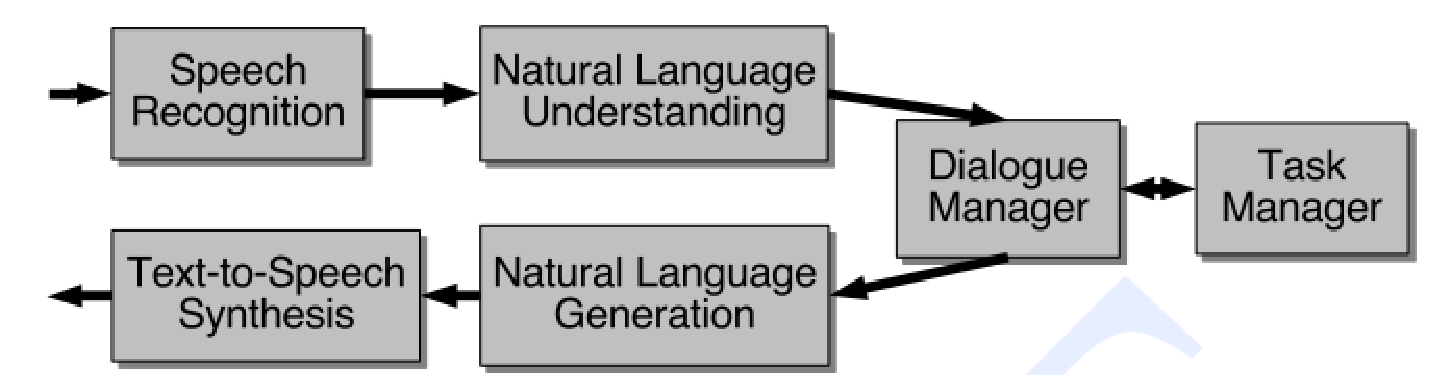
\includegraphics[width=\linewidth]{system_architecture}
  \caption{An example of system architecture}
	\label{system architecture}
\end{figure}

The following sections of this survey paper are organized as follows: From Section \ref{Automatic Speech Recognition} to Section \ref{Text-to-speech Synthesis}, we will introduce the components of goal-driven systems in further detail. Since the TM (task manager) component depends on the specific task at hand, we do not provide any paper about it. In Table \ref{tbl:system_summary}, we summary the technical details of each component used in systems that deployed in real world. We start with each of Section 2-6 a brief summary of the task of the component, and then present related previous work. Finally in Section \ref{Non-goal-driven Systems}, we present some papers about non-goal-driven systems.

\clearpage
\paperwidth 26in
\paperheight 7in
\typearea{33}
\recalctypearea
\begin{table}\label{tbl:system_summary}
\caption{Summary of Goal-oriented Spoken Dialogue Systems}
\begin{tabular}{| p {10em} | p {4em} | p {20em} | p {20em} | p {20em} | p {20em} | p {20em} | p {20em} | p {25em} |}
  \hline
  % after \\: \hline or \cline{col1-col2} \cline{col3-col4} ...
  System & Year & Task Description & Automatic Speech Recognizer (ASR) & Text-to-speech (TTS) & Dialogue Manager (DM) & Natural Language Understanding (NLU) & Natural Language Generation (NLG) & Training Data \\
  \hline
  ConQuest \cite{Bohus2007} & 2007 & Provides technical program information during conferences. Deployed in InterSpeech 2006 and IJCAI 2007. & CMU Sphinx2 \cite{Huang1993}. & Cepstral speech synthesis engine (http://www.cepstral.com). & RavenClaw architecture \cite{Bohus2003}. & Phoenix semantic parser \cite{Ward1994}. & Rosetta, a template-based NLG component. 	& Training data is only used for ASR. It starts with data collected by a text-only prototype. After deployment they collected more data, transcribed it, and retrain the LM. LM used in InterSpeech 2006 were trained on a corpus of 6350 utterances. \\
  \hline
  Let's DiSCoH \cite{Lemon2006} &	2006 &	Users are able to call to learn about a conference, including paper submission, program, venue, etc. Designed to be highly portable and flexible across different conferences and workshops. & \multicolumn{5}{l|}{System developed using the AT\&T VoiceTone Spoken Dialogue System tools \cite{Gilbert2005}, which provides services with ASR, SLU, DM and TTS. System uses a fixed set of responses so no NLG component is mentioned.} &	{LM trained by W99 dataset + artificially generated + data from conference website + manually designed (11,275 + 9,511 + 226 + 467 sentences).} \\
  \hline
  Let's Go \cite{Raux2005} & 2005 & Provide bus schedule information to the Pittsburgh population during off-peak times. & CMU Sphinx2. &	Techniques in Limited Domain Synthesis \cite{Black2000}. Unit selection concatenative voice specifically designed for domain. &	RavenClaw architecture.  &	Initially uses hand-coded Finite State Grammars. Finally uses tri-gram language models trained on artificial corpora. &	Rosetta. &	Data from real world: 614 dialogues, containing 7936 user turns. Manually transcribed and labeled. \\
  \hline
  LARRI \cite{Bohus2002} &	2002 &	A multi-modal system for support of maintenance and repair activities for aircraft mechanics. &	CMU Sphinx2. &	Festival system in a limited domain mode. Use unit-selection synthesizer with a fall back on a diphone voice. &	Behavior is specified through a task-dependent script. AGENDA dialogue manager \cite{Rudnicky1999a}. &	Phoenix semantic parser. &	Rosetta. &	AM trained with WSJ0 corpus. Trigram LM trained with INS BIT Test procedure and general system commands.\\
  \hline
  NJFun \cite{Singh2002} &	2002 &	Provide telephone access to a database of activities in New Jersey. &	Watson Speech Recognizer. &	Concatenative diphone synthesis method. &	Train by reinforcement learning (MDP) Build with DMD scripting language \cite{Levin2003}.	& Watson Speech Recognizer. &	Grammar and template. &	Manually obtained by AT\&T employees. 54 subjects for training and 21 for testing. 311 training dialogues, 124 testing dialogues.\\
  \hline
  CMU Communicator \cite{Rudnicky1999} &	1999 &	\tabincell{p {20em}}{Helps users create complex travel itineraries (multi-leg flights, hotel and car reservations).\\
  \url{http://www.speech.cs.cmu.edu/Communicator/index.html} \\ \\ \\ \\} & \tabincell{l}{CMU Sphinx2.\\ \\ \\ \\ \\} &	\tabincell{l}{Festival system in a limited domain mode\\ with concatenative method. \\ \\ \\ \\} &	\tabincell{l}{Behavior is specified through a task-dependent\\ script. AGENDA dialogue manager.  \\ \\ \\ \\} & \tabincell{l}{Phoenix semantic parser. \\ \\ \\ \\ \\} &	\tabincell{l}{Template-driven.\\ \\ \\ \\ \\} &	\tabincell{l}{Data collected in different stages \cite{Eskenazi1999}:\\
  1)	48 human-human dialogues.\\
  2)	107 Wizard-of-Oz Ver1 (WOZ).\\
  3)	2983 from prototype system, manually transcribed.\\
  4)	16 from WOZ ver2.\\
  Total 3164 dialogues.}\\
  \hline
  \multicolumn{9}{|l|}{There are several other systems whose architectures are similar to that of \cite{Bohus2007, Raux2005, Bohus2002, Rudnicky1999}: RoomLine, Intelligent Procedure Assistant, Vera, MeetingLine, Team Talk, Sublime, Madeleine, RavenCalendar. \url{http://www.cs.cmu.edu/~dbohus/ravenclaw-olympus/systems_overview.html}}\\
  \hline
\end{tabular}
\end{table}

\clearpage
\KOMAoptions{paper=A4,pagesize}
\typearea{18}
\recalctypearea

\section{Automatic Speech Recognition} \label{Automatic Speech Recognition}

The \emph{ASR (automatic speech recognition)} component takes audio input, generally from a telephone, or from a PDA of desktop microphone, and returns a transcribed string of words \cite{Jurafsky2006}.

Most of the successful ASR systems are based on the mathematical foundation of \emph{hidden Markov models (HMM)}. So we begin this section with presenting a tutorial paper of this subject \cite{Rabiner1989A}. The most successful ASR approach has been \emph{HMM-GMM (Gaussian mixture model)}, until the recent emergence of the \emph{HMM-DNN (deep neural network)} approach. The next two sections present two selected papers of the HMM-DNN method \cite{Hinton2012Deep,Graves2013Speech}. The field of ASR has been investigated for many decades, and lots open-source systems are available. Among the many choices, Kaldi \cite{DanielPovey2014} is drawing more and more attentions due to its perfect support for the DNN techniques. In the fourth and the fifth summaries \cite{Mohri2000,Ljolje1999}, we discuss two important topics that are widely applied in the Kaldi system, namely the \emph{weighted finite-state transducer (WFST)} and \emph{lattice}. 

Paper \cite{Stolcke2000} shows that the ASR performance can be further improved, if we can accurately model the conversation in the specific domain, and this paper is also loosely related with the \emph{natural language understanding (NLU)} component.
We then briefly introduce a speaker adaption technique \cite{Leggetter1995}.

\subsection{A tutorial on hidden Markov models and selected applications in speech recognition \cite{Rabiner1989A}}

This paper is a very classic and comprehensive tutorial on \emph{Hidden Markov Models (HMMs)}. Although HMMs is not among the deep learning approaches that emerged in recent years, the concepts behind HMMs are closely related to that of the \emph{Recurrent Neural Networks (RNNs)}.

\begin{figure}[htbp]
  \centering
  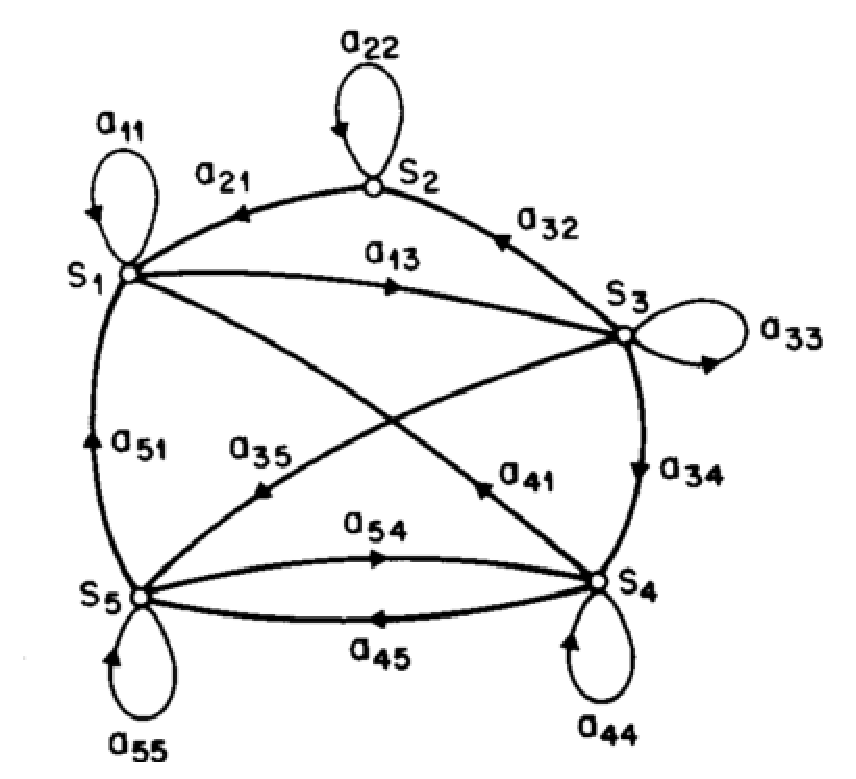
\includegraphics[width=.6\linewidth]{8_29_HMM_chain}\\
  \caption{A Markov chain with 5 states}\label{fig:chain}
\end{figure}

In the discrete Markov processes (without hidden states), a system at any time is described as being in one of a set of distinct state (cf. Figure \ref{fig:chain}). A full probabilistic description of the above system would require specification of the current state, as well as all the predecessor states. For the special case of a discrete, first order, Markov chain, it is assumed that the probabilistic description only depends on the current state and its immediate predecessor. This stochastic process is also called an observable Markov model, since the output of the process is the set of states at each instant of time, where each state corresponds to a physical (observable) event.

HMMs extend the concept to include the case where the observation is a probabilistic function of the hidden states, i.e., the resulting model is a doubly embedded stochastic process with an underlying stochastic process that is not observable, but can only be observed through another set of stochastic processed that produce the observations.

It would be better to explain the concept with the following example. Suppose on the other side of the curtain a person is performing a coin tossing experiment. That person will not tell you anything about what he is doing exactly (he may be tossing 2 or 3 different coins with different biased coins); he will only tell you the result of each coin flip (the observation).

\begin{figure}[htbp]
  \centering
  \subfigure{
    \label{fig:topka} %% label for first subfigure
    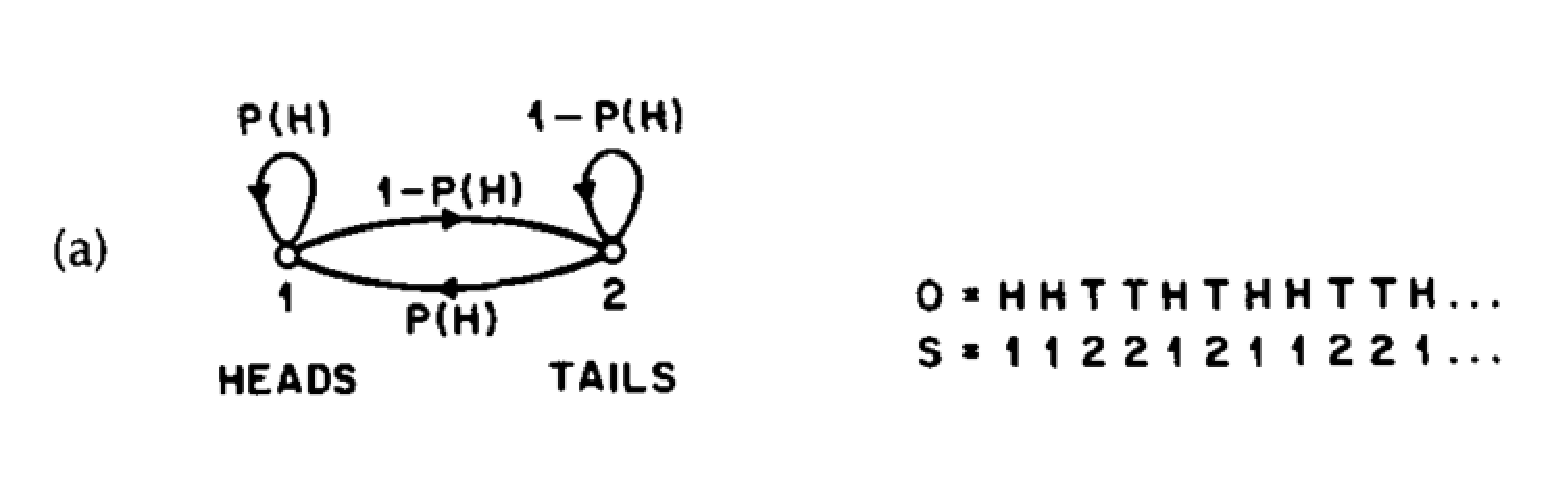
\includegraphics[width=2.2in]{8_29_HMM_coinA}}
  \subfigure{
    \label{fig:topkb} %% label for second subfigure
    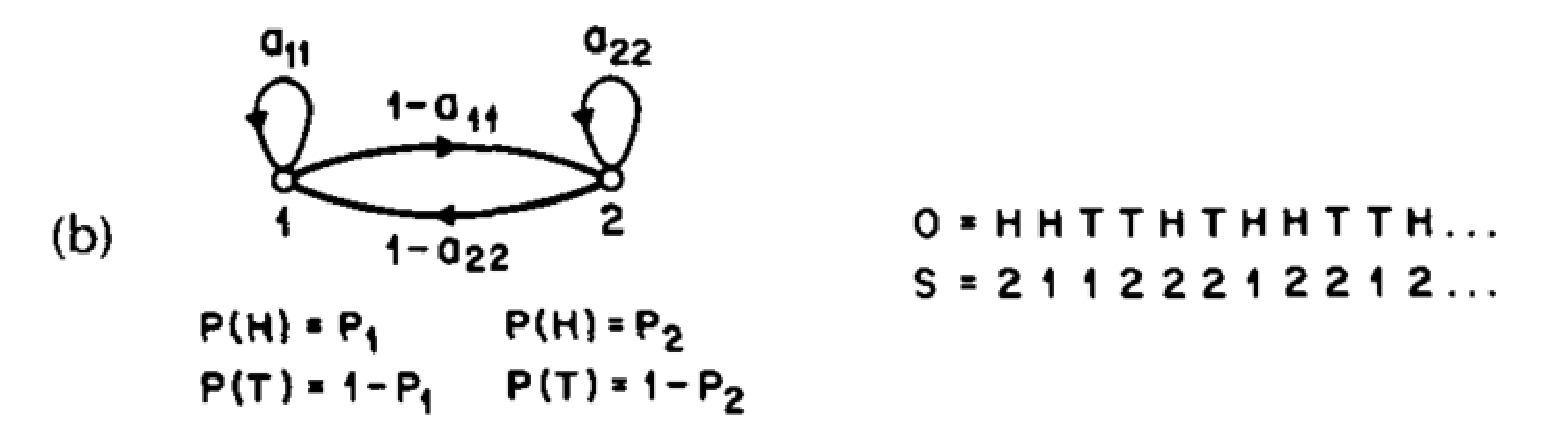
\includegraphics[width=2.2in]{8_29_HMM_coinB}}
  \subfigure{
    \label{fig:topkb} %% label for second subfigure
    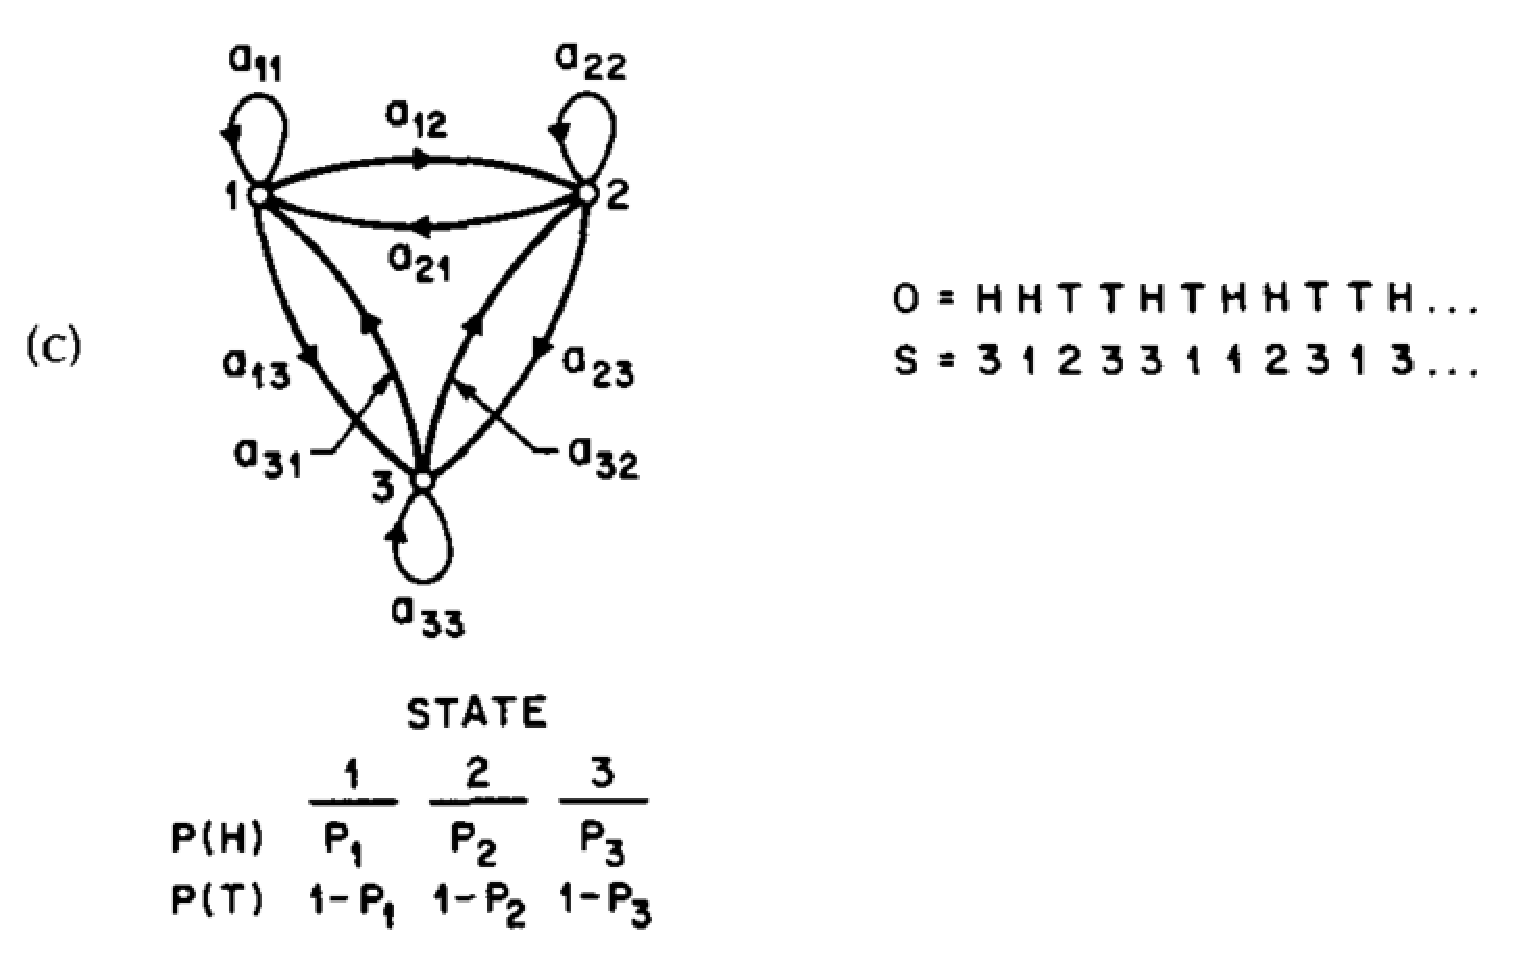
\includegraphics[width=2.2in]{8_29_HMM_coinC}}
  \caption{Three possible Markov models that can account for the results of hidden coin tossing experiments}\label{fig:coin}
\end{figure}

One possible choice would be to assume that only a single coin was being tossed. In this case the situation could be model with a 2-state (fully observable) model where each state corresponds to a side of the coin (cf. Figure \ref{fig:coin} (a)). We can also assume that two different biased coins were being tossed, and use the HMM in Figure \ref{fig:coin} (b) to describe this situation. Here each state corresponds to a different coin. Each state is characterized by a probability distribution of heads and tails, and transitions between states are characterized by a state transition matrix. We could further assume that there are 3 different coins, and model the system as a HMM with 3 hidden states (cf. Figure \ref{fig:coin} (c)).

An HMM is mathematically characterized by the following parameters: 1) $N$, the number of states in the model; 2) $M$, the number of distinct observation symbols; 3) The state transition probability distribution $A=\{a_{ij}\}$; 4) The observation symbol probability distribution in state $j$, $B = \{b_j(k)\}$; 5) The initial state distribution $\pi$. The paper uses the compact notation $\lambda = (A, B, \pi)$ to indicate the complete parameter set of the models.

There are three basic problems for HMMs: 1) How to efficiently compute $P(O| \lambda)$, the probability of the observation sequence given the model; 2) Given the observation sequence $O$ and the model $\lambda$, how to choose a corresponding state sequence $Q$ that is optimal; 3) How to adjust (or train) the parameters in $\lambda$ to maximize $P(O| \lambda)$.

The paper shows that all the three problems can be solved by the \emph{forward-backward procedure}. The basic idea of the forward-backward procedure is to apply the technique of dynamic programming. It introduces a forward variable $\alpha_t(i)$, which is probability of the partial observation sequence $O_1, ..., O_t$ (until time $t$) and state $S_i$ at time $t$. It shows how $\alpha_{t+1}(i)$ can be computed based on $\alpha_t(i)$ (the idea of dynamic programming). Similarly, a backward variable $\beta_t(i)$ is defined as the probability of the partial observation sequence from $t+1$ to the end. Finally, all the three problems can be solve by using the forward and backward variables.

In the remaining parts of the paper, it introduces various types of HMMs that have been previously studied (for example HMMs whose states are not fully connected). It also discusses the issues that arise in implementations, such as initial parameter estimates, model size, missing data, etc. Finally it describes some successful applications of HMMs in the field of speech recognizer. 
\subsection{Deep Neural Networks for Acoustic Modeling in Speech Recognition \cite{Hinton2012Deep}}

This paper provides an overview of the progress of acoustic modeling by \emph{deep neural networks (DNNs)}. It also presents the shared view of four research groups (groups at the University of Toronto, Microsoft Research, Google, and IBM Research) that have had recent successes in using this technique.

The goal of the acoustic modeling in this paper is to determine how well each state of a \emph{hidden Markov model (HMM)} fits a frame or a short window of frames of coefficients that represents the acoustic input $p(HMMstate | AcousticInput)$. So the produced acoustic model is combined with the classic HMM to form the final hybrid \emph{automatic speech recognition (ASR)} system.

In modern ASR systems, the acoustic input is typically represented by concatenating \emph{Mel-frequency cepstral coefficients (MFCCs)} or \emph{perceptual linear predictive coefficients (PLPs)}, computed from the raw waveform and their first- and second-order temporal differences. The preprocessing techniques are designed to discard the large amount of information in waveforms that is considered to be irrelevant for discrimination.

The DNN approach for acoustic modeling has two key stages. In the first stage, layers of feature detectors are initialized, one layer at a time, by fitting a stack of generative models. In the second stage, each generative model in the stack is used to initialize one layer of hidden units in a DNN. Finally the whole network is then discriminatively fine-tuned to predict the target HMM states.

The idea behind the first stage is generative pretraining: it finds a region of the weight-space that allows the discriminative fine-tuning to make rapid progress, and it also significantly reduces overfitting. The generative model in DNN approaches uses a set of parameters, $W$, to define the joint probability of a vector of observable variables $v$, and a vector of latent variables $h$, via an energy function $E$:
$$p(v,h; W) = \frac{1}{Z} e^{-E(v,h; W)}, Z = \sum_{v', h'} e^{-E(v', h'; W)}.$$
In the classic \emph{restricted Boltzmann machine (RBM)} which consists of a layer of stochastic binary visible units and a layer of stochastic binary hidden units, the energy function is defined to be:
$$E(v,h) = -\sum_{i \in  visible} a_i v_u - \sum_{j \in hidden} b_j h_j - \sum_{i,j} v_i h_i w_{ij},$$
where $v_i, h_j$ are the binary states of visible unit $i$ and hidden unit $j$, $a_i, b_j$ are their biases, and $w_{ij}$ is the weight between them. The training of a RBM can be achieved by the \emph{contrastive divergence (CD)} algorithm.

After training an RBM on the data, the inferred states of the hidden units can be used as data for training another RBM that learns to model the dependencies between the hidden units of the first RBM. This can be repeated many times to produce many layers of nonlinear feature detectors, which is called a \emph{deep believe network (DBN)}.

\begin{figure}[htbp]
  \centering
  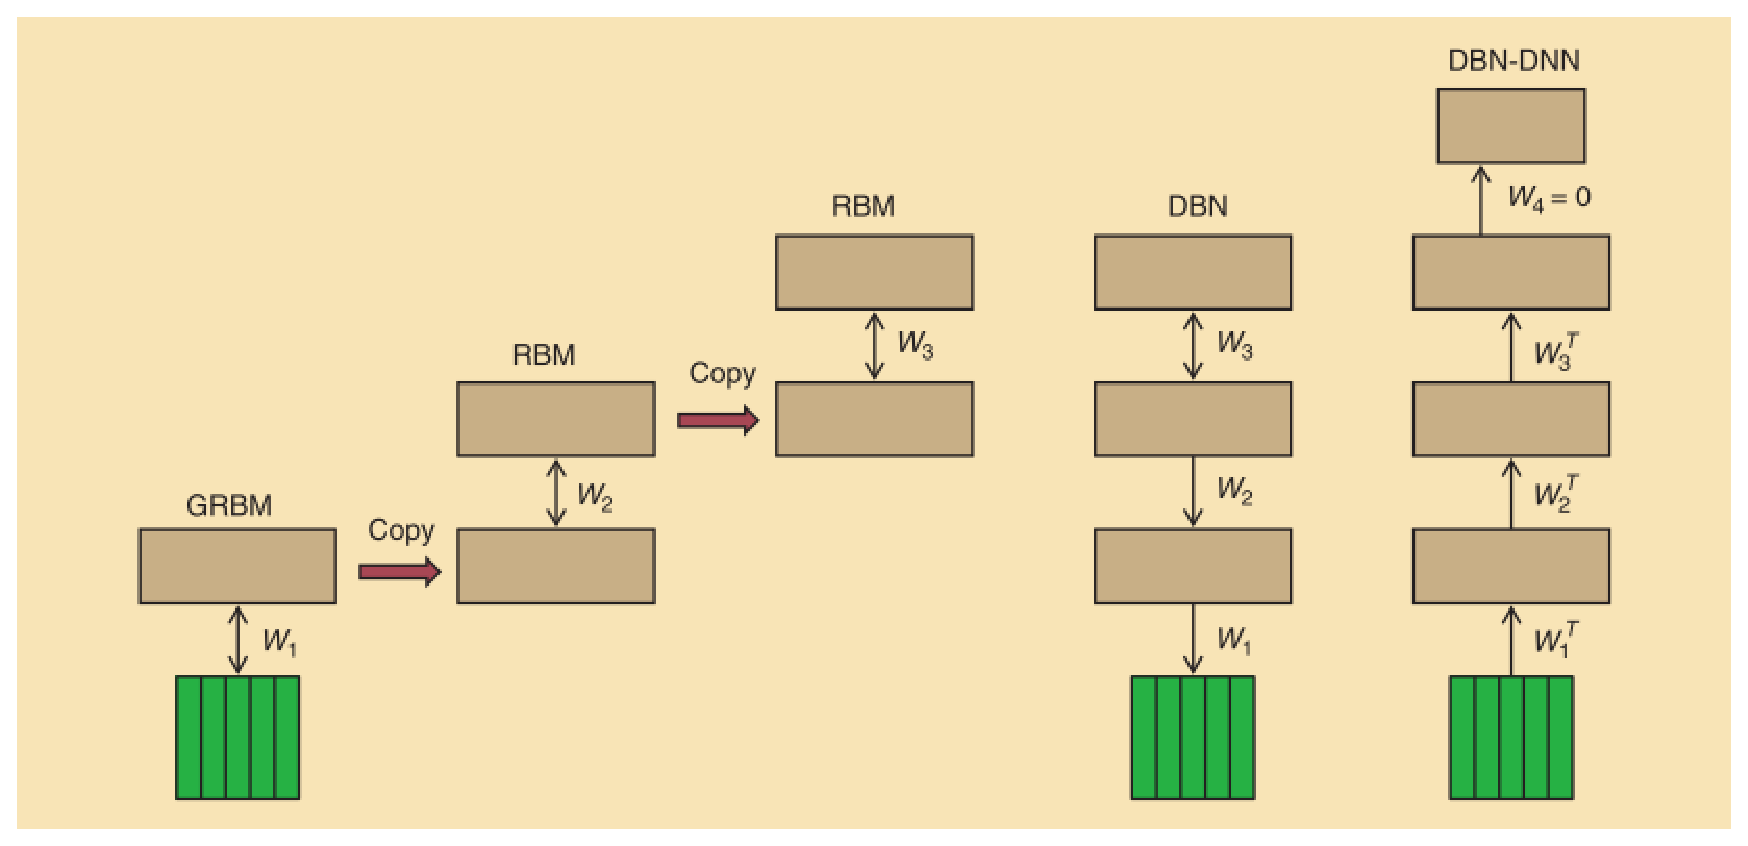
\includegraphics[width=.9\linewidth]{10_17_HMM_DNN}\\
  \caption{Illustration of the DNN training process}\label{fig:HMM_DNN}
\end{figure}

After learning a DBN by training a stack of RBMs, the generative weights in the reverse direction are used as the initialization of a feedforward DNN. It then adds a final softmax layer and trains the whole DNN discriminatively. The whole architecture is illustrated in Figure \ref{fig:HMM_DNN}: 1) A \emph{Gaussian RBM (GRBM)} is trained to model real-valued acoustic coefficients. Then the hidden states of the GRBM are used as data for training the next RBM. 2) This is repeated to create as many hidden layers as desired. 3) Finally, a pretrained DBN-DNN is created by adding a softmax output layer that predicts the hidden state of the HMM.

In the experimental study, the paper reports the results on the TIMIT benchmark and on several large-vocabulary speech recognition datasets. For example in the Bing-voice-search speech recognition task, the best DNN-HMM acoustic model achieves a sentence accuracy of 69.6\% on the test set, compared with 63.8\% for a strong HMM baseline method. 
\subsection{Speech Recognition With Deep Recurrent Neural Networks \cite{Graves2013Speech}}

End-to-end training methods such as \emph{Connectionist Temporal Classification (CTC)} make it possible to train RNNs for sequence labelling problems where the input-output alignment is unknown. However, RNN performance in speech recognition has so far been disappointing. This paper investigates deep recurrent neural networks on the ASR task, and shows that the method achieves a test set error of 17.7\% on the TIMIT phoneme recognition benchmark, which is the best recorded score.

The goal of this paper is to investigate whether RNNs could benefit from depth in space - that is, stacking multiple recurrent hidden layers on top of each other.

\begin{figure}[htbp]
  \centering
  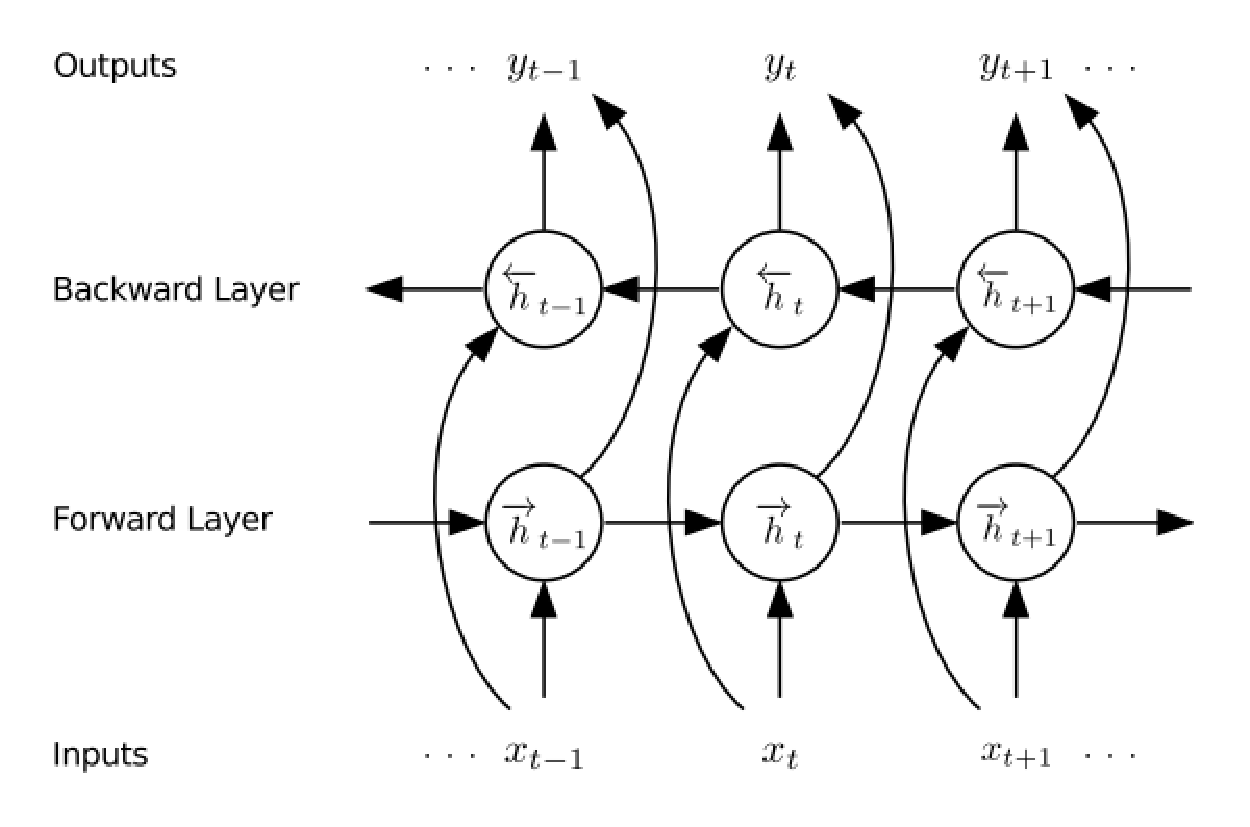
\includegraphics[width=.5\linewidth]{10_17_ASR_RNN}\\
  \caption{Bidirectional RNN}\label{fig:ASR_RNN}
\end{figure}

The concepts of RNN and \emph{long short-term memory (LSTM)} unit have been discussed in previous paper summaries. The basic architecture in this paper is based on the \emph{bidirectional RNNs (BRNNs)}. The basic idea of BRNN is to process the data in both directions (forward and backward) with two separate hidden layers. Figure \ref{fig:ASR_RNN} shows an example of a BRNN model that computes the forward hidden sequence $\stackrel{\rightarrow}{h}$, the backward hidden sequence $\stackrel{\leftarrow}{h}$, and the output sequence $y$. Combining BRNNs with LSTM gives \emph{bidirectional LSTM}.

In the RNN training, the RNNs map directly from acoustic to phonetic sequences. The paper presents two ways to define the output distribution and hence train the network.

The first method is called Connectionist Temporal Classification, which uses a softmax layer to define a separate output distribution $Pr(k|t)$ at every step $t$ along the input sequence. CTC then uses a \emph{forward-backward algorithm} to sum over all possible alignments and determine the normalised probability $Pr(z|x)$ of the target sequence.

The second method is based on the \emph{RNN transducer} technique, which combines a CTC-like network with a separate RNN that predicts each phoneme given the previous ones, thereby yielding a jointly trained acoustic and language model. The basic idea of RNN transducer is to determine a separate distribution $Pr(k | t, u)$ for every combination of input timestep $t$ and output timestep $u$. Specifically, $Pr(k | t, u)$ is defined by taking an `acoustic' distribution $Pr(k | t)$ from the CTC network, a `linguistic' distribution $Pr(k | u)$ from the prediction network, then multiplying them together and renormalising.

In the experimental study, the proposed model is evaluated on the TIMIT corpus. It is reported that the \emph{phoneme error rate (PER)} on the core test set is 17.7\%, which is the best result known to the authors.

Remark: I have also consider the possibility of applying RNNs on the ASR task. This paper shows that this is indeed a promising approach. Compared to the HMM-based or hybrid methods, the approach of this paper is simpler and more elegant - it can jointly train the acoustic and language models in an end-to-end fashion. However, this method is still not very mature, since the TIMIT benchmark is restricted in size. As mentioned by the authors, a possible future work is to extend the system to large vocabulary speech recognition. 
\subsection{Speech Recognition with Weighted Finite-State Transducers \cite{Mohri2000}}

This paper describes a general representation and algorithmic framework for speech recognition based on \emph{weighted finite-state transducers (WFST)}. These transducers provide a common and natural representation for major components of speech recognition systems, including \emph{hidden Markov models (HMMs)}, context-dependency models, pronunciation dictionaries, etc. The paper shows the application of the proposed method to large-vocabulary recognition task.

A \emph{finite-state transducer} is a finite automaton whose state transitions are labeled with both input and output symbols. Therefore, a path through the transducer encodes a mapping from an input symbol sequence, or string, to an output string. A weighted transducer puts weights on transitions in addition. In this paper, weights encode the probabilities that accumulates along the path.

\begin{figure}[h]
  \centering
  % Requires \usepackage{graphicx}
  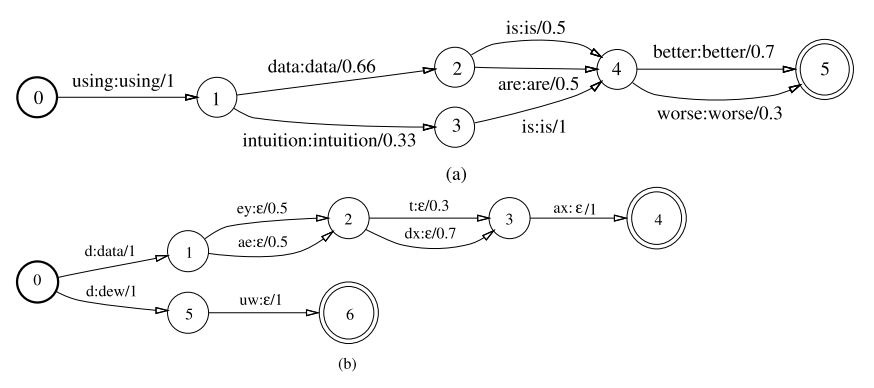
\includegraphics[width=\linewidth]{11_21_WFST.png}\\
  \caption{Examples of weighted finite-state transducer}\label{fig:WFST}
\end{figure}

Figure \ref{fig:WFST} presents a toy language model and a toy pronunciation lexicon as WFSTs. In Figure \ref{fig:WFST}(b), the WFTS maps from phone strings to words in the lexicon, in this example `data' and `dew', with probabilities representing the likelihoods of alternative pronunciations. Similarly, HMM structures can be combined into a single transducer that preserves phone model identity.

The proposed method relies on a common set of weighted transducer operations to combine, optimize, search and prune them. The basic operations \emph{union}, \emph{concatenation}, and \emph{Kleene closure} operations combine transducers in parallel, in series, and with arbitrary repetition, respectively. There are three other key operations that are used in the speech applications:

1) \emph{Composition}: Composition is the transducer operation for combining different levels of representation. For example, a pronunciation lexicon can be composed with a word-level grammar to produce a phone-to-word transducer. In particular, the composition $T = T_1 \circ T_2$ has exactly one path mapping string $u$ to string $w$ for each pair of paths, the first in $T_1$ mapping $u$ to $v$ and the second in $T_2$ mapping $v$ to $w$.

2) \emph{Determinization}: In a deterministic transducer, each state has at most one transition with any given input label and there are no input $\epsilon$-labels. The key advantage of a deterministic transducer is its irredundancy: it contains at most one path matching any given input string, thereby reducing the time and space needed to process the string. The determinization algorithm transforms a non-deterministic WFST into an equivalent deterministic WFST.

3) \emph{Minimization}: Given a deterministic WFST, its size can be reduced by minimization, which can save both space and time. Let the given WFST be denoted as $A$. The minimization algorithm results in a WFST $B$ that is equivalent to $A$, and has the least number of states and the least number of transitions among all deterministic WFSTs equivalent to $A$.

Next we will see how to construct a single recognition transducer that maps from context-dependent phones to a string of words.

Consider the pronunciation lexicon $L$ in Figure \ref{fig:WFST}(b), and the grammar $G$ of Figure \ref{fig:WFST}(a). $L \circ G$ gives a transducer that maps from phones to word strings restricted to the grammar $G$. If we let $C$ represent a transducer from context-dependent phones to context-independent phones, then $C \circ (L \circ G)$ gives a transducer that maps from context-dependent phones (such as triphones) o word strings restricted to the grammar $G$. Finally, the transducer is optimized with determinization and minimization: $N = min(det(C \circ (L \circ G)))$.

In the following sections, the paper introduces the operation algorithms in further details, and reports the experimental results in the large-vocabulary speech recognition task. It is shown that the proposed method can greatly improve the efficiency and save space. 
\subsection{Efficient General Lattice Generation and Rescoring \cite{Ljolje1999}}

This paper describes a lattice generation method that produces high-quality lattices with less than 10\% increased computation over standard \emph{Viterbi} decoding. The proposed method is closely related to previous lattice generation methods, but applies to more general network topologies.

\begin{figure}[h]
  \centering
  % Requires \usepackage{graphicx}
  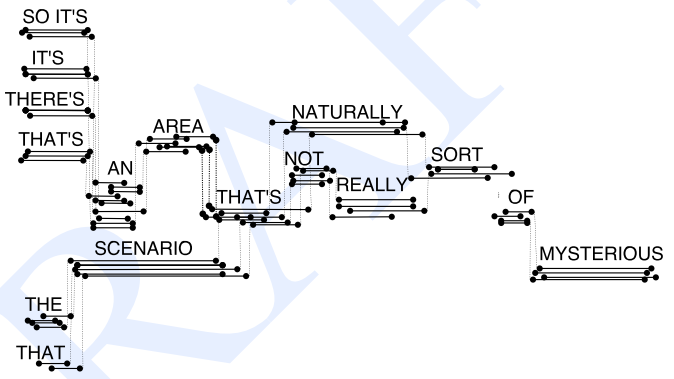
\includegraphics[width=.7\linewidth]{11_21_lattice.png}\\
  \caption{Example of a lattice}\label{fig:lattice}
\end{figure}

In this paper, a \emph{lattice} is defined to be a labeled, weighted, directed acyclic graph in which each complete path represents an alternative transcription hypothesis, weighted by its recognition score for a given utterance. However, it should be noted that there is no generally accepted single definition of lattice. Figure \ref{fig:lattice} shows an example of lattice (figure from Chapter 10 of Speech and Language Processing \cite{Jurafsky2006}).

In this paper, \emph{ASR networks} are represented as \emph{finite-state transducers}. These are labeled, weighted, directed graphs in which each arc $a$ has a source state $S(a)$, destination state $D(a)$, an input label $I(a)$, output label $O(a)$, and a weight $P(a)$. Here each input label is a context-dependent phone symbol, and each output label is a word. A complete path through such a transducer gives a legal sequence of words in the language model.

The recognition task can be characterized as finding a path $a = a_1,...,a_n$ that maximizes the joint probability of the acoustic and language models when applied to a given utterance:
$$\max_a P(\vec{x}[0, \tau], a) = \max_{a, t_1, ..., t_{n-1}}\prod_{i=1}^n P(\vec{x}[t_{i-1}, t_i] | I(a_i)) P(a_i).$$

The first factor represents the acoustic model likelihood for the context-dependent phone $I(a_i)$, and the second factor represents the language probability for that arc in the transducer $T$. Let $B(s)$ be the set of all paths in $T$ from the initial state to state $s$. Define
$$\alpha(s,t) = \max_{a \in B(s), t_1, ..., t_{k-1}} \prod_{i=1}^k P(\vec{x}[t_{i-1}, t_i] | a_i) P(a_i).$$
Then:
$$\max_{a} P(\vec{x}[0,t], a) = \max_{D(a)=s} p(a) [\max_{t' < t} P(\vec{x}[t',t]|I(a)) \alpha(S(a), t')].$$
In this way, the familia Viterbi recursion is factored into two nested loops: the outer loop considers each possible active arc $a$ ending in $s$, and the inner loop picks out the optimal start time $t'$.

The lattice generation algorithm consists of three main steps: 1) creates a context-dependent phone-to-word transducer lattice; 2) converts it to a word lattice; 3) prunes the lattice relative to the best scoring path.

In the first step, each state in lattice $L$ corresponds to a pair $(t,s)$ of a time frame in the recognition and a state from the transducer $T$. If during the Viterbi recursion, it has identified the optimal start time $t'$ for are $a$ ending in state $D(a)$ at time $t$, then a corresponding arc is added to $L$ from $(t', S(a))$ to $(t, D(a))$.

To convert the phone-to-word lattices to word lattices, it relies on the efficient implementations of the general finite-state operations. It deletes the input labels by the projection operator, and removes the $\epsilon$ arcs.

The final step is to prune the lattice relative to the best scoring path. The method is simple: the best score $\alpha(s)$ among paths from the initial state to state $s$ is found, as well as the best score $\beta(s)$ among paths from state $s$ to a final state. State for which $\alpha(s) + \beta(s) < \kappa \times \beta(s_0)$ are then pruned.

In the experimental section, it is shown that lattice generation requires typically less than 10\% additional computation time above one-best decoding. With the second pass, the proposed method is able to achieve a 3x real-time word error rate of 11.2\% on the Eval'95 test set. 
\subsection{Dialogue Act Modeling for Automatic Tagging and Recognition of Conversational Speech \cite{Stolcke2000}}

This paper describes a statistical approach for modeling \emph{dialogue acts (DAs)} on conversational speech, i.e., speech-act-like units such as \emph{Statement}, \emph{Question}, \emph{Backchannel}, etc. The proposed model detects and predicts dialogue acts based on lexical, collocational, and prosodic cues, as well as on the discourse coherence. It develops a probabilistic integration of speech recognition with dialogue modeling, to improve both speech recognition and dialogue act classification accuracy.

The goal of this paper is twofold: 1) presets a comprehensive framework for modeling and automatic classification of DAs, and proposes a framework that provides a mathematically principled way to condition the speech recognizer on conversation context through dialogue structure; 2) presents results obtained with this approach on a large, widely available corpus of spontaneous conversational speech.

This paper follows a recent standard for shallow discourse structure annotation, the \emph{Dialogue Act Markup in Several Layers (DAMSL)} tag set, which aims to provide a domain-independent framework for dialogue annotation.

The mathematical and computational framework used in the paper is the \emph{hidden Markov model (HMM)}. Given all available evidence $E$ about a conversation, the goal is to find the DA sequence $U$ that has the highest posterior probability $P(U|E)$ given that evidence.
$$U^* = \arg\max_U P(U|E) = \arg\max_U P(U) P(E|U).$$
Next we will discuss the prior probability $P(U)$, and the posterior probability $P(E|U)$ respectively.

In modelling the prior distribution $P(U)$, the paper assumes that the distribution is Markovian, i.e., each $U_i$ depends only on a fixed number $k$ of preceding DA labels:
$$P(U_i | U_1, ..., U_{i-1}) = P(U_i | U_{i-k}, ..., U_{i-1}).$$
The paper trains standard backoff N-gram models, using the frequency smoothing approach. The authors also tried several alternative approaches, but there was no significant improvement over the simple N-gram method.

The computation of $P(E|U)$ depends on the types of evidence use. The paper used the following three types of sources of evidence, either alone or in combination:
\begin{itemize}
\item{\textbf{Transcribed words}\\
$P(W|U)$, where $W$ refers to the true (hand-transcribed) words spoken in a conversation.
}
\item{\textbf{Recognized words}\\
A standard approach is to use the 1-best hypothesis. A more thorough approach is to compute $P(A|U)$ (where $A$ is the acoustics input) by decomposing it into an acoustic likelihood $P(A|W)$ and a word-based likelihood $P(W|U)$:
$$P(A|U) = \sum_W P(A|W) P(W|U).$$
}
\item{\textbf{Prosodic features}\\
$P(F|U)$, where $F$ are the features capturing various aspects of pitch, duration, energy, etc., of the speech signal. For the prosodic classifiers, the paper used CART-style decision trees. One example in the corpus was the distinction between backchannels and agreement. The prosodic tree trained on this task is shown in Figure \ref{fig:stolcke00-decision_tree}. The paper also tried to use neural network classifiers on this task, and tested
various network structures. However, there was no encouraging result.
\begin{figure}[h]
  \centering
  % Requires \usepackage{graphicx}
  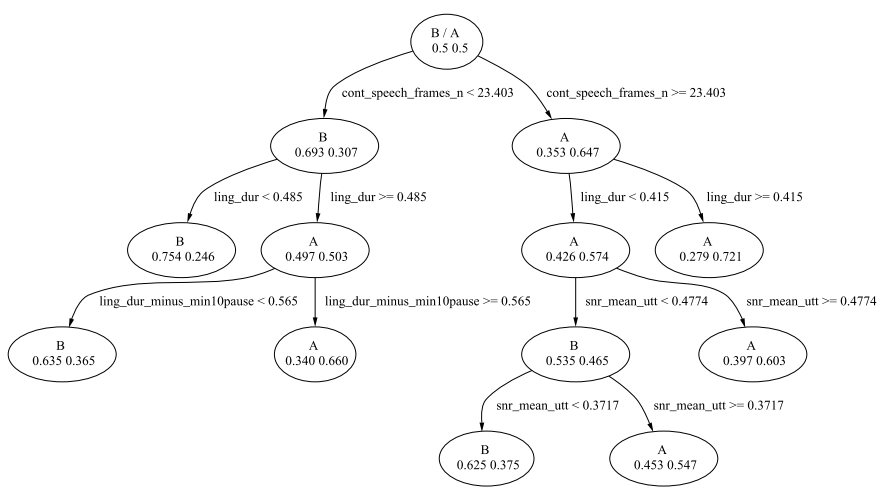
\includegraphics[width=\linewidth]{stolcke00-decision_tree.png}\\
  \caption{Decision tree for the classification of backchannels and agreements.}\label{fig:stolcke00-decision_tree}
\end{figure}
}
\end{itemize}

The paper proposes a method to combine multiple knowledge source, by using the following approximation:
\begin{align*}
P(A_i, W_i, F_i | U_i) &= P(A_i, W_i | U_i) P(F_i | A_i, W_i, U_i)\\
                       &\approx P(A_i, W_i | U_i) P(F_i | U_i).
\end{align*}

The HMM representation allows using efficient dynamic programming algorithms to compute relevant aspects of the model, such as: 1) the most probable DA sequence (the \emph{Viterbi algorithm}); 2) the posterior probability of various DAs for a given utterance (the \emph{forward-backward algorithm}).

The paper considers ways to use DA modeling to enhance automatic speech recognition (ASR). The first method is called \emph{mixture-of posteriors}, which yields:
$$P(W_i | A_i, E) = \sum_{U_i} \frac{P(W_i | U_i) P(A_i | W_i)}{P(A_i | U_i)} P(U_i | E).$$
The second method, called \emph{mixture-of-LM}, results in:
$$P(W_i | A_i, E) \approx (\sum_{U_i} P(W_i | U_i) P(U_i|E)) \frac{P(A_i |W_i)}{P(A_i)}.$$

The experiments confirmed that DA modeling can improve word recognition accuracy quite substantially in principle, at least for certain DA types.But the skewed distribution of DAs limits the usefulness of the approach on the Switchboard corpus. The paper suggests that the benefits of DA modeling might be more pronounced on corpora with more even DA distribution, which is typically the case for task-oriented dialogues.

\subsection{Maximum Likelihood Linear Regression for Speaker Adaption of Continuous Density Hidden Markov Models \cite{Leggetter1995}}

Adaption techniques fall into two main categories - speaker normalization in which the input speech is normalized to match the speaker that the system is trained to model, and model adaptation techniques in which the parameters of the model set are adjusted to improved the modelling of the new speaker. This paper proposes a model adaptation technique which uses a set of regression-based transforms to tune the hidden Markov model (HMM) mean parameters to the new speaker.

The basic idea of the maximum likelihood linear regression (MLLR) method is to calculate the transformation matrices to maximize the likelihood of the adaptation data, and can be implemented using the forward-backward algorithm. By tying the transformations among a number of distributions, adaptation can be performed for distributions which are not represented in the training data.

Consider a continuous density HMM system with Gaussian output distribution. A particular distribution, $s$ is characterized by a mean vector, $\mu_s$, and a covariance matrix $C_s$. Given a parameterized speech frame vector $o$, the probability density of the vector is
$$b_s(o) = \frac{1}{(2\pi)^{n/2} |C_s|^{1/2}} e^{-\frac{1}{2(o - \mu_s)'G_s^{-1}(o-\mu_s)}}.$$

The adaptation of the mean vector is achieved by applying a transformation matrix $W_s$ to the extended mean vector $\xi_s$ to obtain an adapted mean vector $\hat{\mu_s}$: $\hat{\mu_s} = W_s \xi_s$. Here $\xi_s$ is defined as $\xi_s = [\omega, \mu_1, ..., \mu_n]'$, where $\omega$ is the offset term for the regression. For distribution $s$, the probability density function for the adapted system becomes
$$b_s(o) = \frac{1}{(2\pi)^{n/2} |C_s|^{1/2}} e^{-\frac{1}{2(o - W_s \xi_s)'G_s^{-1}(o-W_s \xi_s)}}.$$

A more general approach is that the same transformation matrix is used for several distributions. The transformation is estimated using data from all the associated tied distributions, so if some of the distributions are not observed in the adaptation data, a transformation may still be applied. The degree of transformation tying is determined by the amount of adaptation data available. For the case of small amounts of adaptation data a global transformation may be used.

The following sections of this paper describes the method in further details, specifically proposes how to use to forward-backward algorithm to train the transformation matrix.

In the experimental study, it is shown that with the proposed method adaptation can be performed using as little as 11s of adaptation data, and that as more data is used the adaptation performance improves. For example, using 40 adaptation utterances, a 37\% reduction in error from the speaker-independent system was achieved with supervised adaptation and a 32\% reduction in unsupervised mode. 


\section{Natural Language Understanding}

The \emph{NLU (natural language understanding)} component of dialogue system produces a semantic representation which is appropriate for the dialogue task. Many speech-based dialogue systems are based on the frame-and-slot semantics \cite{Jurafsky2006}. In this circumstance, the task of NLU is equivalent to filling each slot with the correct value, given the information from the upstream ASR component.

In this section, we begin with presenting some classic approaches for NLU, based on rules, grammar and statistic learning \cite{Miller1996,Pieraccini1994,Ward1994}. Although these methods look simple, they suffice to build several non-trivial dialogue systems that are deployed in real world. The work of Rayner \cite{Rayner2003} aims to proposed a method that can combine both the power of rule-based and data-driven approaches. Several other deep learning techniques proposed recently are also closely related with the NLU component \cite{Hermann2013, Kalchbrenner2013}.

In another line of research, NLU is not restricted to discover merely the value of each slot, but take a more ambitious step to translate the given natural sentence to formal logic or database queries \cite{Grefenstette2014}. These NLU techniques are not yet widely applied in SDS.

Another subject closely related to NLU is called the \emph{dialogue state tracking challenge (DSTC)}. We conclude this section with a paper that address the challenge with LSTM network \cite{Zilka2015} which shows that the NLU component is not always necessary.

\subsection{A Fully Statistical Approach to Natural Language Interfaces \cite{Miller1996}}

This paper presents a natural language interface system which is based entirely on trained statistical models. The system consists of three stages of processing: \emph{parsing}, \emph{semantic interpretation}, and \emph{discourse}. Each of these stages is modeled as a statistical process. The models are fully integrated, resulting in an end-to-end system that maps input utterances into meaningful representation frames.

The focus of this paper is to extract sufficient information from each utterance to give an appropriate response to a user's request. The model structure of this paper is described as follows: Given a string of input words $W$ and a discourse history $H$, the task of statistical language understanding system is to search among the many possible discourse-dependent meanings $M_D$ for the most likely meaning $M_0$:
$$M_0 = \mathop{\arg \max}_{M_D} P(M_D | W, H).$$
Let $T$ denote a semantic parse tree, and $M_S$ denote pre-discourse sentence meaning (the sentence meaning without considering the discourse history) we can introduce intermediate levels into the statistical framework:
$$M_0 = \mathop{\arg \max}_{M_D} \sum_{M_S, T} P(M_D | W, H, M_S, T) P(M_S, T | W, H).$$

The representation can be further simplified with the following three assumptions: 1) Neither the parse tree $T$, nor the pre-discourse meaning $M_S$, depends on the discourse history $H$. 2) The post-discourse meaning $M_D$ does not depend on the words $w$ or the parse structure $T$, once the pre-discourse meaning $M_S$ is determined. 3) The probability of words $W$ does not depend on meaning $M_S$, given that parse $T$ is known. Finally, these assumptions yield the following objective function:
$$M_0 = \mathop{\arg \max}_{M_D} (\max_{M_S, T}(P( M_D | H, M_S) P(M_S, T) P(W | T))).$$
\begin{figure}[h]
  \centering
  % Requires \usepackage{graphicx}
  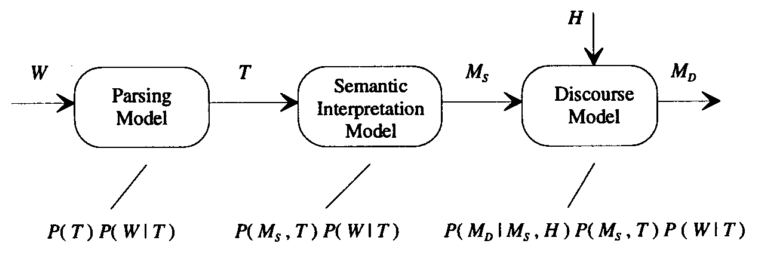
\includegraphics[width=.9\linewidth]{stat_NLI1.png}\\
  \caption{Overview of statistical processing}\label{fig:stat_NLI1}
\end{figure}

This expression corresponds to the computation actually performed by the system which is shown in Figure \ref{fig:stat_NLI1}. The processing proceeds in three stages:
\begin{enumerate}
\item Word string $W$ arrives at the parsing model. The fill space of possible parses $T$ is searched for $n$-best candidates according to the measure $P(T)P(W|T)$. These parses, together with their probability scores, are passed to the semantic interpretation model. The probability $P(T)$ is modeled by state transition probabilities in a recursive transition network, and $P(W|T)$ is modeled by word transition probabilities. Here state transition probabilities have the form $P(state_n | state_{n-1}, state_{up})$, and word transition probabilities have the form $P(word_n | word_{n-1}, tag)$.
\item The constrained space of candidate parses $T$, combined with the full space of possible pre-discourse meanings $M_S$, is searched for $n$-best candidates according to the measure $P(M_s, T)P(W|T)$. These pre-discourse meanings, together with their associated probability scores, are passed to the discourse model. Both pre-discourse and post-discourse meanings in the current system are represented using a simple frame representation (cf. Figure \ref{fig:stat_NLI2}). The problem in this stage is to compute the prior probability of meaning $M_S$ and parse $T$ occurring together. The method of this paper is to embed the instructions for constructing $M_S$ directly into parse $T$. So the probability $P(M_S, T)$ is then simply the prior probability of producing the augmented tree structure.
    \begin{figure}[h]
      \centering
      % Requires \usepackage{graphicx}
      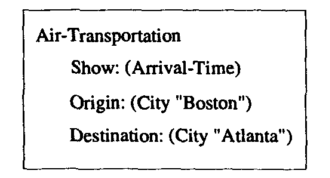
\includegraphics[width=.4\linewidth]{stat_NLI2.png}\\
      \caption{A sample semantic frame}\label{fig:stat_NLI2}
    \end{figure}
\item The constrained space of candidate pre-discourse meanings $M_S$, combined with the full space of possible post-discourse meanings $M_D$, is searched for the single candidate that maximizes $P(M_D | H, M_S)P(M_S, T)P(W|T)$, conditioned on the current history $H$. The discourse history is then updated and the post-discourse meaning is returned. The discourse history $H$ simply consists of the list of all post-discourse frame representations for all previous utterances in the current session. Let $M_P$ denote the last frame in the list. The statistical discourse model maps a 23 element input vector onto a 23 element output vectors. Here $X$ represents the combination of $M_P$ and $M_S$, while $Y$ represents the post-discourse meaning $M_D$. Finally, the probability $P(Y | X)$ is determined by a statistical decision tree model.
\end{enumerate}

In the experimental study, the paper trained and evaluated the system on a common corpus of utterances collected from naive users in the \emph{ATIS} domain. The combined system produced an error rate of 21.6\%, and work on the system was still ongoing. 
\subsection{A Learning Approach to Natural Language Understanding \cite{Pieraccini1994}}

This paper proposes a learning paradigm for the problem of understanding spoken language. The basis of the work is in a formalization of the understanding problem as a communication problem. The resulting understanding algorithm consists in a Viterbi maximization procedure analogous to that commonly used for recognizing speech.

The first step of this paper is to formalize the NLU problem as a \emph{communication problem}. Two assumptions are made in this step: 1) the meaning of a sentence can be expressed by a sequence of basic units $\mM = \mu_1, ..., \mu_{N_M}$, and there is a sequential correspondence between $\mu_j$ and a subsequence of the acoustic observation $A = a_1, ..., a_{N_a}$; 2); 2) the second assumption is to think of the acoustic representation as a version of the original sequence of meaning units corrupted by a noisy channel. Thus for a given acoustic observation $A$, the problem of understanding a sentence can be expressed as finding $\mathop{\max\arg}_\mM P(\mM | A)$.

A simple choice is to define a unit of meaning as a keyword/value pair $m_j = (k_j, v_j)$, where $k_j$ is a conceptual category (e.g. origin, meal) and $v_j$ is the value in the actual sentence (e.g. Boston, breakfast). In what follows we use $W = w_1, ..., w_{N_W}$ to denote the sequence of words, and use $C = c_1, ..., c_{N_W}$ to denote the sequence of concept labels.

Using the Bayesian rule, the formula can be expressed as:
$$\mathop{\max\arg}_{W,C} P(A | W, C) P(W | C) P(C).$$
It is further assumed that:
$$P(w_i | w_{i-1}, ..., w_1, C) = P(w_i | w_{i-1}, ..., w_{i-n+1}, c_i),$$
$$P(c_i | c_{i-1}, ..., c_1) =  P(c_i | c_{i-1}, ..., c_{i-m}).$$
When $n=m=1$, this is equivalent to a first order \emph{hidden Markov model (HMM)}.

\begin{figure}[h]
  \centering
  % Requires \usepackage{graphicx}
  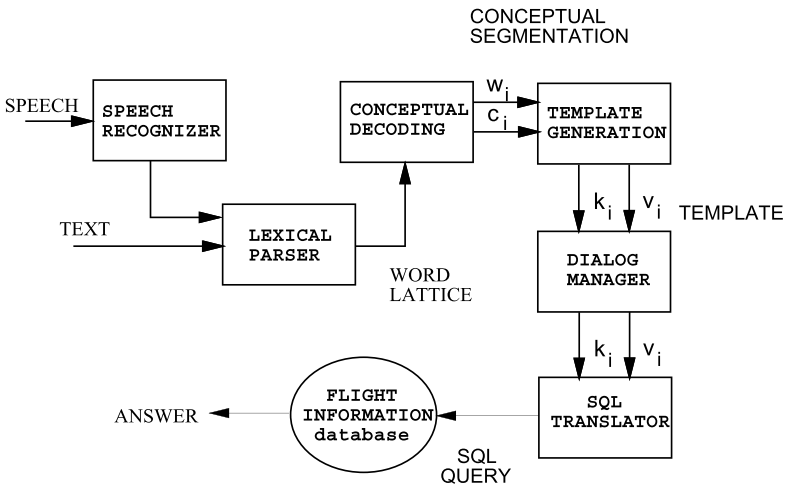
\includegraphics[width=.8\linewidth]{P94-NLU_diag.png}\\
  \caption{Block diagram of the understanding system.}\label{fig:P94-NLU_diag}
\end{figure}

The paper then presents how to implement this idea and apply it to the \emph{ATIS (Air Travel Information System)} corpus. A block diagram of the speech understanding system is presented in Figure \ref{fig:P94-NLU_diag}. Next we will see each of the components in further detail.

In the \emph{conceptual decoding} module, the paper proposes to impose a certain structure to the HMM. It is observed that in a typical sentence there are phases that generally represent the question, a subject and finally a restriction. So the HMM follows this structure to alleviates the problems of the locality of the model and that of concept embedding.

The \emph{lexical parser} dues with different issues related with spoken language, such as the representation of numbers and acronyms. The lexical parser also deletes articles (i.e. THE and A), since they play no role in the conceptual decoding process.

The paper uses the most natural way of \emph{interfacing} the conceptual decoder with a speech recognizer, by directly implementing the maximization of the probability described above. In order to manage the model size, it uses only those words and bigrams that were observed in the training data.

The goal of the \emph{template generator} module is to analyze the conceptual segmentation, and generate the final representation of the meanings. Finally values are assigned to the decoded concepts according to the result of a pattern matching procedure. However, the design of pattern matching tables still requires manual efforts.

The \emph{dialog manager} implements the function of recording the dialog history, and generates proper responses. The simple strategy used in the paper is to keep a current context template, with all the information that has been used. If a concept is mentioned in a new sentence but with a different value, all concepts in the context template at a lower hierarchical level are deleted.

In the experimental study, the proposed system was evaluated on a set of 687 sentences called February 92 test set. The results on the test set from text input account for 68\% of correct answers, 18\% wrong answers and 14\% rejects. When the system was coupled with a speech recognizer through the best first hypothesis, the performance dropped to 52\% of correct answers, 26\% wrong answers and 22\% rejects.

\subsection{Recent Improvements in the CMU Spoken Language Understanding System \cite{Ward1994}}

A spoken language system needs to recognize and understand spontaneous speech, which often contains disfluencies and ungrammatical construction. The goal of this paper is to develop a NLU system that can respond appropriately to input, even though coverage is not complete.

The CMU NLU system is called \emph{Phoenix}, which has a loose coupling between the speech recognizer. The recognizer uses stochastic language models to produce a single word string hypothesis. This hypothesis is then passed to a parsing module which uses semantic grammars to produce a semantic representation for the input utterance.

The basic idea of this paper is to use a flexible frame-based parser, which parses as much of the input as possible. The Phoenix system uses \emph{Recursive Transition Networks} to encode semantic grammars. The grammars specify word patterns which correspond to semantic tokens understood by the system. A subset of tokens are considered as top-level tokens, which means they can be recognized independently of surrounding context. Nets call other nets to produces a semantic parse tree. The top-level tokens appear as slots in the frame structures. There is not one large sentential-level grammar, but separate grammars for each slot (there are approximately 70 of these in the ATIS system). The parser is flexible at the slot level in that it allows slots to be filled independent of order.

The parser operates by matching the word patterns for slots against the input text. A set of possible interpretations are pursued simultaneously. The system is implemented as a top-down Recursive Transition Network chart parser for slots. As slot fillers are recognized, they are added to frames to which they apply. At the end of an utterance the parser picks the best scoring frame as the result. The output of the parser is the frame name and the parse trees for its filled slots.

The semantic grammar used for parsing in the ATIS task is developed by processing transcripts of subjects performing scenarios. The data consists of around 20,000 utterances, and a subset of this data (around 10,000 utterances) has been annotated. However, it has a problem with the grammar coverage if it misses one of the content words in the utterance. The paper tries to solve this problem by generalizing the grammar to parse strings that are syntactically similar to the utterances in the training data.

The paper also found it helpful to pursue alternate interpretations, which are not the best according to the heuristics used by the parser. This is achieved by generating a beam of interpretations. The parser still produces the single best interpretation, but keeps track of a number of others. Whenever the backend notices a problem, it asks the parser for another interpretation.

In the experimental study, it is reported that the error rates of the speech recognizer, NLU component and the overall system are 4.4\%, 9.3\% and 13.2\% respectively.

\subsection{Transparent Combination of Rule-based and Data-driven Approaches in a Speech Understanding Architecture \cite{Rayner2003}}

This paper describes a domain-independent semantic interpretation architecture suitable for spoken dialogue systems, which uses a decision-list method to effect a transparent combination of rule-based and data-driven approaches.

The goal of the paper is to propose an architecture which combines rule-based and data-driven methods as transparently as possible. This will allow the system to shift smoothly from an initial version which is entirely rule-based, to a final version which is largely data-driven.

In this paper, \emph{semantic interpretation} is viewed as a statistical \emph{classification} task. There is a set of semantic atoms, each representing a primitive domain concept, and a semantic representation is defined to be a non-empty set of semantic atoms. For example, the semantic representation of the utterance ``show me the sample syringe'' is $\{show, sample\_syringe\}$. As well as specifying the permitted semantic atoms themselves, it also defines a target model which for each atom specifies the other atoms with which it may legitimately combine. For example, $minutes$ may only combine with $correction$, $set\_alarm$ or a number.

Training data consists of a set of utterances, in either text or speech form, each tagged with its intended semantic representation. The paper defines a set of feature extraction rules, each of which associates an utterance with zero or more features. Statistics are then compiled to estimate the probability $p(a | f)$ of each semantic atom $a$ given each separate feature $f$.

In the decoding process, the system is given an utterance $u$, to which the system assigns a representation $R(u)$ consisting of a set of semantic atoms, together with a target model. The decoding process  proceeds as follows:
\begin{enumerate}
\item Initialise $R(u)$ to the empty set.
\item Use the feature extraction rules and the compiled statistics to find the set of triples $\langle f, a, p \rangle$ where $f$ is a feature associated with $u$, $a$ is a semantic atom, and $p$ is the probability $p(a | f)$.
\item Order the set of triples by the value of $p$, with the largest probabilities first.
\item Remove the highest-ranked triple $\langle f,a,p \rangle$ from $T$. Add $a$ to $R(u)$ if the probability $p$ is greater than some threshold and $a$ is consistent with $R(u)$.
\end{enumerate}

The paper describes an open-source toll called $ALTERF$, which implements the abstract procedure introduced above. It shows how the $ALTERF$ system processes the training data, and decodes the given utterance in running time with further details.

In the experimental study, the paper shows that when all the training data is used, the combined system outperforms the rule-based system by 22.2\% to 27.3\%, and outperforms the N-gram system by 22.2\% to 25.6\%. It shows that the proposed method can get a significant improvement on rules-based technique by adding a trainable component. 
\subsection{Multilingual Distributed Representations without Word Alignment \cite{Hermann2013}}

This paper proposes a method for learning distributed representations in a multiligual setup. The model learns to assign similar embeddings to aligned sentences and dissimilar ones to sentences which are not aligned. It shows that the representations are semantically informative and applies them to a cross-lingual document classification task.

The basic idea is that, given enough parallel data, a shared representation would be forced to capture the common elements between sentences from different languages. What two parallel sentences have in common, of course, is the semantics of those two sentences. Using such parallel data, it proposes a novel method for learning vector representations at the word level and beyond.

The first step is to define a bilingual error function as follows: given a \emph{compositional sentence model (CVM)} $\mM_A$, which maps a sentence to a vector, it trains a second CVM $\mM_B$ using a parallel corpus $\mC_{A,B}$. For each pair of parallel sentences $(a,b) \in \mC_{A,B}$, it attempts to minimize
$$E_{dist}(a,b) = ||a_{root} - b_{root}||^2,$$
where $a_{root}$ ($b_{root}$) is the vector representing sentence $a$ ($b$).

The CVM used in this paper is a simple additive composition function:
$$a_{root}= \sum_{i=0}^{|a|} a_i.$$
Due to the use of parallel data, we know that $a$ and $b$ are semantically equivalent. Hence the goal is to jointly train both models $\mM_A$ and $\mM_B$, so that
$$E_{bi}(\mC_{A,B}) = \sum_{(a,b) \in \mC_{A,B}} E_{dist}(a,b)$$
is minimized.

However, the models could learn to reduce all embeddings and composition weights to zeros and thereby minimize the objective function. This problem is addressed by penalizing small distances between non-parallel sentence pairs. For every pair of parallel sentences $(a,b)$ it samples a number of additional sentences $n \in \mC_B$, which are not exact translation of $a$:
$$E_{noise}(a, b, n) = [1 + E_{dist}(a,b) - E_{dist}(a,n)]_{+},$$
where $[x]_{+} = \max(x,0)$ denotes the standard hinge loss. Thus, the final objective function is defined to be:
$$J(\theta_{bi}) = \sum_{(a,b) \in \mC_{A,B}} (\sum_{i=1}^k E_{noise}(a,b,n_i)) + \frac{\lambda}{2} || \theta_{bi} ||^2.$$

\begin{figure}[h]
  \centering
  % Requires \usepackage{graphicx}
  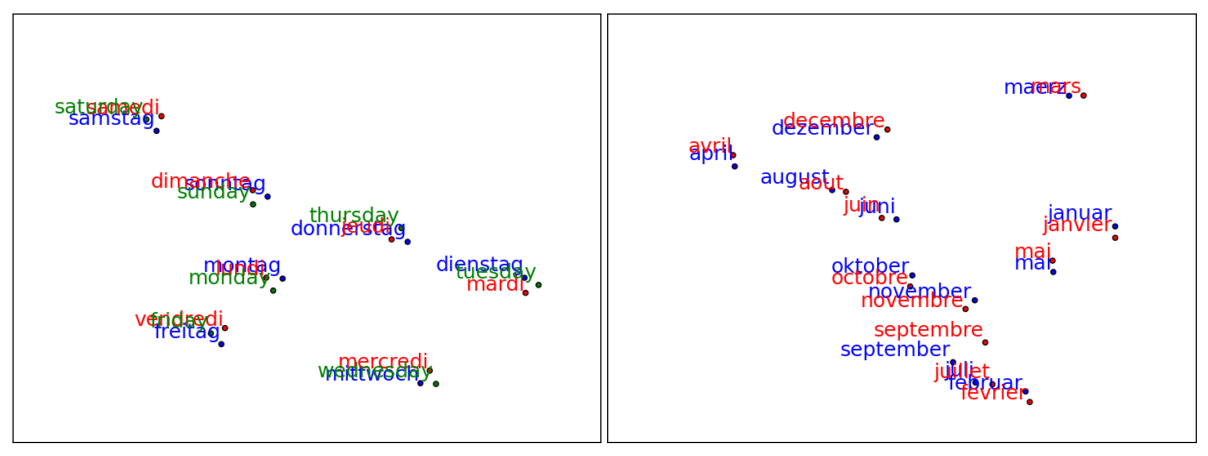
\includegraphics[width=\linewidth]{Hermann13-BiCVM.png}\\
  \caption{The left scatter plot shows t-SNE projections for a weekdays in three language. The right plots shows months using only the German and French words.}\label{fig:Hermann13-BiCVM}
\end{figure}

In the experimental study, the paper evaluates the proposed model in to experiments: the \emph{BiCVM} model was trained on 500k sentence pairs of a English-German parallel corpus. The \emph{BiCVM+} used this dataset in combination with anther 500k parallel sentences form the English-French section. The motivation behind BiCVM+ is to investigate whether it can learn better embeddings by introducing additional data in a different language. The models are evaluated on the \emph{cross-lingual document classification (CLDC)} task. It is shown that both models outperform all prior work on this task. Further, BiCVM+ outperforms BiCVM, indicating the usefulness of adding training data from a separate pair. Figure \ref{fig:Hermann13-BiCVM} shows the t-SNE projections for a number of English, French and German words.

\subsection{Recurrent Convolutional Neural Networks for Discourse Compositionality \cite{Kalchbrenner2013}}

This paper introduces both a sentence model and a discourse model corresponding to the two levels of compositionality: cords combine to form the meaning of sentences, and sentences combine to form the meaning of dialogues. The sentence model adopts convolution as the central operation, and is based on a novel \emph{hierarchical convolutional neural network (HCNN)}. The discourse model extends the sentence model, and is based on a \emph{recurrent neural network (RNN)}.

The basic kernel operation used in HCNN is described as follows. Given a sentence $s$ and its paired matrix $\mathbf{M}^s$, let $\mathbf{m}$ be a feature that is a row in $\mathbf{M}^s$. Let $w_1, ..., w_k$ be a sequence of $k$ weights. The local weighted addition over the first $k$ values is:
$$y = w_1 \mathbf{m}_1 + ... + w_k \mathbf{m}_k.$$
Then a kernel simply defines the value of $k$, and the one-dimensional convolution applies local weighted addition to each subsequence of values of $\mathbf{m}$. The one-dimensional convolution ($\mathbf{k} * \mathbf{m}$) is defined as:
$$(\mathbf{k} * \mathbf{m})_i = \sum_{j=1}^k \mathbf{k}_j \cdot \mathbf{m}_{k+i-j}.$$

To define the hierarchical architecture of the model, the paper next defines a sequence of kernel sizes and associated weights. Let $l$ be the number of words in the sentence $s$. The sequence of kernel sizes is defined as
$$k_1^l = 2, k_{i+1}^l = k_i^l + 1, k_t^l = l - \sum_{j=1}^{t-1}(k_j^l - 1).$$
That is, kernel sizes increase by one until the resulting convolved vector is smaller or equal to the last kernel size (cf. Figure \ref{fig:Kal13-hier}).

\begin{figure}[h]
  \centering
  % Requires \usepackage{graphicx}
  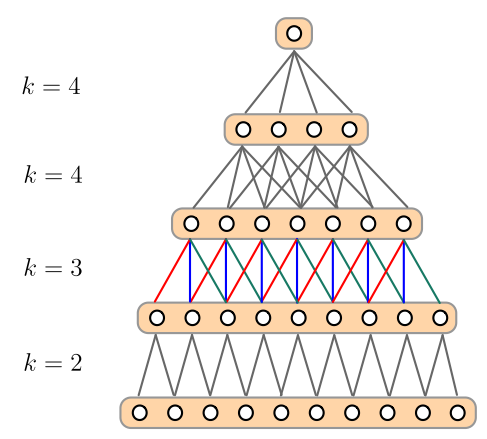
\includegraphics[width=.6\linewidth]{Kal13-hier_HCNN.png}\\
  \caption{A hierarchical convolutional neural network for sentential compositionality.}\label{fig:Kal13-hier}
\end{figure}

The composition operation in HCNN is formally defined as follows. For each feature $f$, let $\mathbf{K}_i^f$ be a sequence of $t$ kernels, where the size of the kernel $|\mathbf{K}_i^f| = k_i^l$. The hierarchy of matrices and corresponding features are defined as:
\begin{align*}
\mathbf{M}_{f,:}^1 &= \mathbf{M}_{f,:}^s,\\
\mathbf{M}_{f.:}^{i+1} &= \sigma(\mathbf{K}_i^f * \mathbf{M}_{f,:}^i + b_f^i).
\end{align*}

The discourse model adapts a RNN architecture in order to capture central properties of discourse. The proposed method aims to capture at least two of the most prominent properties: the sequentiality of the utterances, and the interactions between the speakers.

The RNN architecture takes inputs from a HCNN conditioned on the respective speakers. Let $s_1, ..., s_T$ be a sequence of sentences, each in turn being a sequence of words $s_i = y_1 ... y_l^i$. Let $x_1, ..., x_T$ be a sequence of labels, and $a_1, ..., a_T$ be a sequence of speaker. The RNN computes probability distribution by iterating the following equations:
\begin{align*}
\mathbf{h}_i &= \sigma(\mathbf{I} x_{i-1} + \mathbf{H}^{i-1}\mathbf{h}_{i-1} + \mathbf{Ss}_i + b_h)\\
         p_i &= softmax(\mathbf{O}^i \mathbf{h}_i + b_o)
\end{align*}

\begin{figure}[h]
  \centering
  % Requires \usepackage{graphicx}
  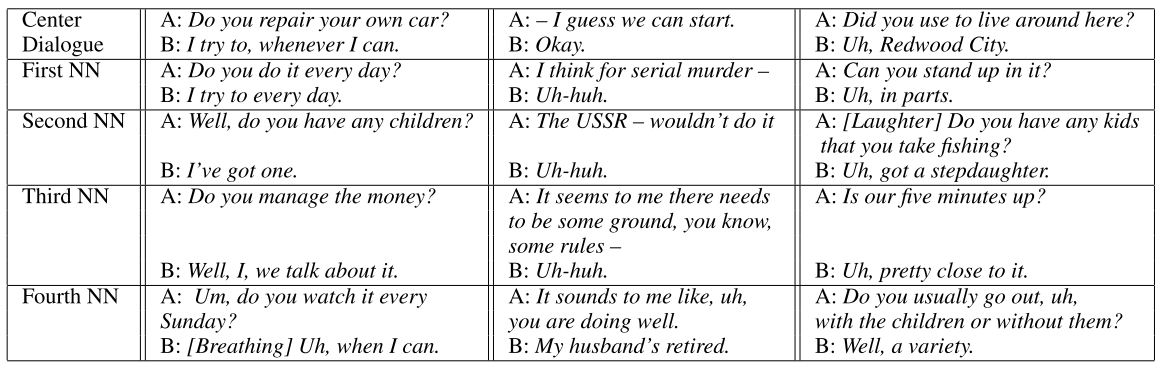
\includegraphics[width=\linewidth]{Kal13-NN.png}\\
  \caption{Short dialogues and nearest neighbours.}\label{fig:Kal13-NN}
\end{figure}

In the experimental study, the paper evaluates the proposed model with the prediction of dialogue acts within the \emph{Switchboard Dialogue Act corpus}. The RCNN model achieves prediction accuracy of 73.9\%, while the best previous result was 71.0\%. Figure \ref{fig:Kal13-NN} shows three randomly chosen dialogues, and the four nearest neighbours of each.

\subsection{A Deep Architecture for Semantic Parsing \cite{Grefenstette2014}}

This paper presents a novel deep learning architecture which provides a semantic parsing system through the union of two neural models of language semantics. It allows for the generation of ontology-specific queries from natural language statements and questions without the need for parsing, which makes it especially suitable to grammatically malformed or syntactically atypical text such as tweets.

The goal of \emph{semantic parsing} is to map natural language sentences to formal representations of their underlying meaning. Within the context of question answering - the focus of this paper - semantic parsing typically aims to map natural language to database queries that would answer a given question.

The model proposed in the paper borrows from two approaches in the deep learning literature: the \emph{Bilingual Compositional Sentence Model (BiCVM)} and \emph{Conditional Neural Language Model (CNLM)}.

\begin{figure}[h]
  \centering
  % Requires \usepackage{graphicx}
  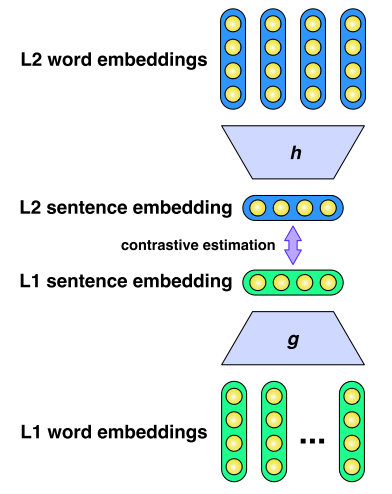
\includegraphics[width=.5\linewidth]{G2014-BiCVM.png}\\
  \caption{Diagrammatic representation of a BiCVM.}\label{fig:BiCVM}
\end{figure}

The BiCVM model shown in Figure \ref{fig:BiCVM} assumes vector composition functions $g$ and $h$, which map an ordered set of word embeddings onto a single vector. For semantically equivalent sentences $a, b$ across different languages (for example English and Chinese), the model aims to minimise the distance between these composed representations:
$$E_{bi}(a,b) = ||g(a) - h(b)||^2.$$
This error is combined with a noise-contrastive hinge loss, where $n$ is a randomly sampled sentence dissimilar to the parallel pair $\{a,b\}$, and $m$ denotes some margin:
$$E_{hl}(a,b,n) = max(0, m + E_{bi}(a,b) - E_{bi}(a,bn)).$$

A \emph{log-bilinear language model} is a neural network modelling a probability distribution over the next word in a sequence given the previous $n-1$, i.e. $p(w_n | w_{1:n-1})$. Let $C_i$ be the context transform matrix which modifies the representation of the $i$th word in the word history. Let $b_{w_i}$ be a scalar bias associated with a word $w_i$, and $b_R$ be a bias vector associated with the model. A log-bilinear model expressed the probability of $w_n$ as a function of the energy of the network:
$$E(w_n ; w_{1:n-1}) = -(\sum^{n-1}_{i=1}R_{w_i}^T C_i) R_{w_n} - b_R^T R_{w_n} - b_{w_n}.$$
To reframe a log-bilinear language model as a CNLM, the simplest way is to do this additively, which allows us to treat the contribution of the conditional variable $\beta$ as an extra word in the history.

The models described above can be combined to form a model capable of jointly learning a shared latent representation for question/query pairs using a BiCVM, and using this latent representation to learn a conditional log-bilinear CNLM.

\begin{figure}[h]
  \centering
  % Requires \usepackage{graphicx}
  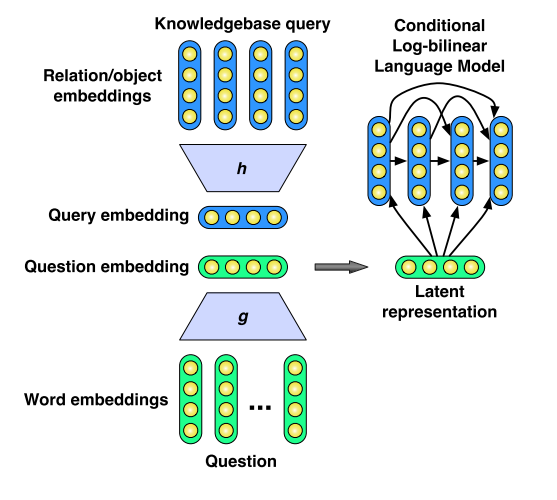
\includegraphics[width=.6\linewidth]{G2014-combined.png}\\
  \caption{Diagrammatic representation of the combined model.}\label{fig:G2014-combined}
\end{figure}

Figure \ref{fig:G2014-combined} shows the combined model. For the natural language side of the model, the composition function $g$ can be a simple additive model. Function $h$, which maps the knowledge base queries into the shared space could use a convolution neural network. Using function $g$ and the original training data, the training data for the second stage is created by obtaining the latent representation for the questions of the original dataset. Once trained, the models can be fully joined to produce a generative neural network.

Finally, the paper suggests that the proposed model can be trained in a two-stage process, and discusses the experimental requirements. However, there is no implementation when the paper is published. So it is left as future work whether the proposed training method can yield fruitful results in practice.

\subsection{Incremental LSTM-based Dialog State Tracker \cite{Zilka2015}}

A dialog state tracker estimates the user's goal throughout the dialog by analyzing the \emph{automatic speech recognition (ASR)} outputs for the user's utterance. This paper presents an incremental dialog state tracker based on LSTM networks. It directly uses ASR hypothesis to track the state.

Because of uncertainty in the user input, statistical dialog systems maintain a distribution over all possible states, called the belief state. In this paper, a dialog state at time $t$ is defined as a vector $s_t \in C_1 \times ... \times C_k$ of $k$ dialog state components (sometimes also called slots). Each component $c_i \in C_i = \{ v_1, ..., v_{n_i} \}$ takes one of $n_i$ values. The goal of the dialog state tracker is to give the probability distribution over one of the independent components $p(c_i | w_1, ..., w_t)$.

\begin{figure}[h]
  \centering
  % Requires \usepackage{graphicx}
  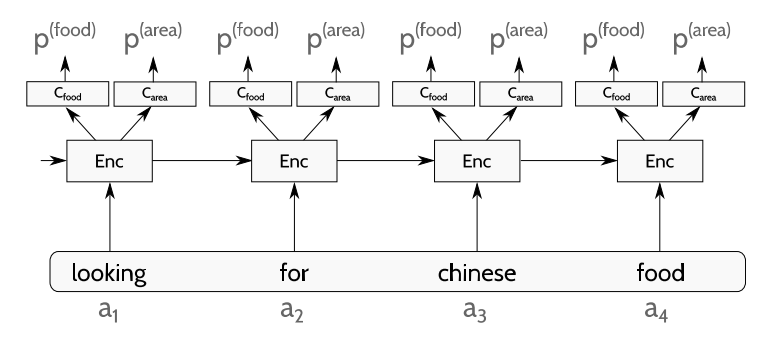
\includegraphics[width=.7\linewidth]{11_28_dstc_ilstm.png}\\
  \caption{A demonstration of the proposed model}\label{fig:dstc_ilstm}
\end{figure}

The main idea of this paper is to use LSTM to encode the information from the input word sequence into a fixed-length vector representation. Given this representation, a classifier returns a probability distribution over the value of the dialog state. An example of the model applied to a particular input sentence is at Figure \ref{fig:dstc_ilstm}.

Formally, the input neural network maps the word $a$ and its ASR confidence score $r$ to a joint representation $u$: $u = NN(a, r)$. The representation $u$ is used by the LSTM encoder along with the previous hidden state $q_{t-1} = (c_{t-1}, h_{t-1}$ to create a new hidden state $q_t$: $q_t = Enc(u, q_{t-1})$. The classifier, represented by a single softmax layer, then maps the hidden state to a probability distribution over all possible values: $p_t = C(h_t)$.

The training criterion is a cross-entropy loss for a dialog example, which is annotated by true labels at some points in time:
$$l(\theta) = - \sum_{t \in Y} \log LecTrack(a_1, r_1, ..., a_n, r_n)_{y_t}^t,$$
where $y_i$ denotes a label for the dialog state at time $i$, and $Y$ is a set of times where the label $y_i$ exists.

In the experimental study, the paper shows that the propose model yields performance to the state-of-the-art system. For example in the requested component, the proposed method achieves 0.98 accuracy and 0.04 L2 score, which is identical to the result of the previous best system. 

\section{Dialogue Manager}

The \emph{DM (dialogue manager)} component typically deals with (1) \emph{state tracking}, which refers to representing information from the past as dialogue states; (2) \emph{action selection} or \emph{dialogue strategy}, which refers to mapping from dialogue states to system actions.

Hand-crafting the dialogue strategy in DM can be quite labor intensive. In order to alleviate the painstaking human efforts, several DM architectures and frameworks are proposed, aiming to allow rapid development of dialog management components for spoken dialog systems operating in complex, goal-oriented domains \cite{Bohus2003,Rudnicky1999a}

Two more sophistigated and successful approaches for strategy learning are \emph{Markov decision process (MDP)} \cite{Levin2000A} and \emph{partially observable Markov decision process (POMDP)} \cite{Young2013Pomdp, Gasic2011}. MDP learns to map dialogue states to actions and does not model the uncertainty about states. To tackle the problem, POMDP maintains a distribution over dialogue, i.e. \emph{belief state}, and based on the distribution actions are chosen. Both MDP and PMDMP methods need to learn in an interactive manner. Schatzmann et al. present a survey of the simulated users \cite{Schatzmann2006}, which are commonly used to create the interactive environment.

The far-reaching deep learning techniques are also significantly influencing the DM research. Williams et. al propose to automatically infer state representation using neural networks \cite{Williams2016End}. Similarly, several other end-to-end systems reach promising performance without hand-crafted features for dialogue states \cite{Bordes2016Learning}. Recurrent neural networks are used to learn how to update the state in a data-driven manner \cite{Henderson2014Word}. Dhingra et al. present a method that combines the reinforcement technique with deep learning \cite{Dhingra2016End}, which is used to built a dialogue agent that provides users with an entity from a knowledge base.

\subsection{RavenClaw: Dialog Management Using Hierarchical Task Decomposition and an Expectation Agenda \cite{Bohus2003}}

This paper describes \emph{RavenClaw}, a new dialog management framework used in the \emph{CMU Communicator}. RavenClaw introduces a clear separation between task and discourse behaviour specification, and allows rapid development of dialog management components for spoken dialog systems operating in complex, goal-oriented domains.

Dialog management maintains continuity over turns in a conversation between human and computer. The authors believe that the essence of dialog management resides in performing two functions: interpreting user inputs with respect to tasks within the domain, and maintaining the coherence over time. Based on this philosophy, the proposed RavenClaw is a two-tier architecture (cf. Figure \ref{fig:raven_arch}). The \emph{Dialog Task Specification} layer captures all the domain-specific dialog logic. The \emph{Dialog Engine} is a domain-independent component that controls the dialog and contributes basic conversational strategies (e.g., timing and turn-taking behaviour, grounding behaviour, etc.).

\begin{figure}[h]
  \centering
  % Requires \usepackage{graphicx}
  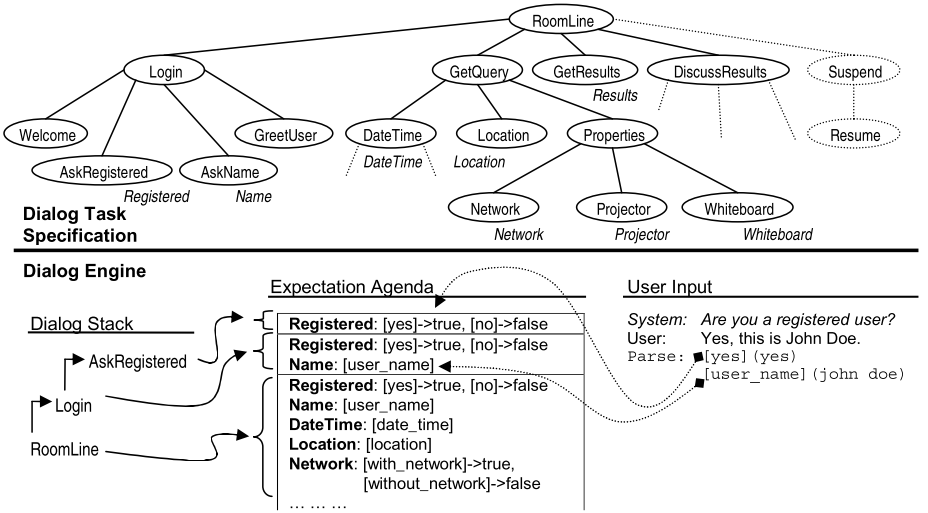
\includegraphics[width=\linewidth]{ravenclaw_arch.png}\\
  \caption{RavenClaw architecture.}\label{fig:raven_arch}
\end{figure}

The domain-specific dialog control is represented in the Dialog Task Specification level using a tree of dialog agents, with each agent handling a certain part of the dialog task. The proposed architecture uses hierarchical task decompositions, which are traditionally used for task execution in robotics. Two categories of dialog agents populate the task tree: \emph{fundamental dialog agents} and \emph{dialog agencies}. The fundamental dialog agents appear as leaf nodes (e.g. \textbf{Welcome}, \textbf{AskRegistered}) and represent atomic dialog actions. The non-terminal nodes in the tree are dialog agencies (e.g. \textbf{Login}, \textbf{GetQuery}), which control the execution of their subsumed agents, capturing the higher level temporal and logical structure of the dialog task.

The Dialog Engine is the core component in RavenClaw and controls the dialog by executing the Dialog Task Specification. Dialog flow is generated by interleaving \emph{Execution Phases} and \emph{Input Phases}. In an Execution Phase, the various agents in the task tree are executed and generate the system's behaviour. In an Input Phase, the system collects and incorporates the information from the user's input.

A characteristic which greatly influences the usability and ultimately the success of spoken dialog systems is their ability to employ a rich set of conversational strategies. These encompass grounding behaviours (e.g. confirmations, disambiguations, etc.), turn-taking and timing behaviours. RavenClaw provides automatic support for all the above mentioned conversational strategies. Internally, they are implemented as dialog agencies, in the same manner as the domain-specific dialog task tree.

Finally, the paper presents five systems using RavenClaw-based dialog managers (LARRI, the Intelligent Procedure Assistant, BusLine, RoomLine and TeamTalk). These implemented systems show that the proposed framework can be easily adapted to different domains, indicating that RavenClaw is with a high degree of versatility and scalability.

\subsection{An Agenda-based Dialog Management Architecture for Spoken Language Systems \cite{Rudnicky1999a}}

This paper proposes a dialog management architecture based on the elements of \emph{handlers}, a \emph{product} and an \emph{agenda}. The goal is to develop a dialog management that can solve two specific problems: 1) providing a coherent coverall structure to interaction that extends beyond the single turn; 2) correctly manage mixed-initiative interaction.

When the paper was written there were two commonly used dialog management approaches: \emph{graph-flow based} systems and \emph{frame-based} systems. Graph-based systems handle the dialog by explicitly enumerating all possible dialog states, as well as allowable transitions between states. However, graph systems have a number of limitations, such as making it difficult for a user to change topic. The frame-based method does not necessarily extend to more complex tasks, for example ones where the goal is to create a complex data object, such as a plan.

The paper first describes a \emph{script-based dialog manager}, before formally introducing the more sophisticated agenda-based architecture. Script in the context simply refers to an explicit sequencing of task-related topics. Each topic is expressed as a form-filling task. In the control strategy, slots are pre-ordered based on their ability to constrain the solution; this ordering provides a default sequence in which the system selects to ask the user about. Figure \ref{fig:R99a-script_based} shows the structure of the Flight Leg topic in the script-based system.

\begin{figure}[h]
  \centering
  % Requires \usepackage{graphicx}
  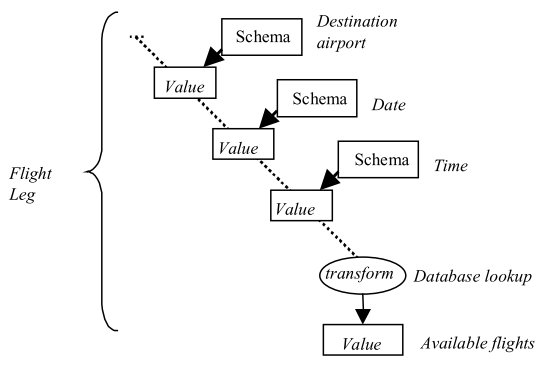
\includegraphics[width=.6\linewidth]{R99a-script_based.png}\\
  \caption{Task-based dialog control in a script-based system.}\label{fig:R99a-script_based}
\end{figure}

The script-based approach still has a number of limitation, such as making it difficult to navigate over the product. So the paper further proposes an \emph{agenda-based} architecture.

The proposed architecture introduces two new data structures: an \emph{agenda} to replace a fixed script, and a \emph{dynamic product} that could evolve over the course of a session. In the agenda-based system, the product is represented as a tree, which reflects the natural hierarchy and order of the information needed. A dynamic product is simply one that can be modified over the course of a session.

Operationally, this means providing a set of operators over tree structures and making these available to the user and to the system. Each node in the product tree corresponds to a handler, which encapsulates computation relevant to a single information item. The agenda is an ordered list of topics, represented by handlers that govern some single item or some collection of information. The agenda specifies the overall ``plan'' for carrying out a task.
The handler on the top of the agenda has the highest priority and represents the focused topic. When a user input comes in, the system calls each handler per their order in the agenda, and each handler will try to interpret the user input and generate the response.

The proposed dialog management architecture is implemented in the \emph{CMU Communicator} system, which handles a complex travel task consisting of air travel, hotels and car reservations. The system uses the \emph{Sphinx II} speech recognizor in a real-time mode and supports barge-in. A top-1 hypothesis is produced by the decoder and parsed by \emph{Phoenix} using a semantic domain-specific grammar. The example dialog presented in the paper shows a number of features of the proposed architecture: the ability to absorb implicit changes of topic on the part of the user, adding to an existing itinerary, and handling explicit topic shifts.

\subsection{A stochastic model of human-machine interaction for learning dialog strategies \cite{Levin2000A}}

This paper proposes a quantitative model for dialog systems that can be used for learning the dialog strategy. After formalising the dialog design as a \emph{Markov decision process (MDP)}, the reinforcement learning algorithm is used to find the optimal strategy. This approach is evaluated in an \emph{air travel information system (ATIS)} task.

The key idea of this paper is to formalise the dialog design as an optimization problem with an objective function reflecting different dialog dimensions for a given application. With some assumptions about the state transition probabilities and cost assignment, a dialog system can be mapped to a MDP, which has a variety of data driven algorithms for finding the optimal strategy.

The first step is to state the problem of dialog design as optimization of an objective $C$:
$$C = \sum W_i \langle C_i \rangle,$$
where the terms $\langle C_i \rangle$ are the expected costs for different dialog dimensions. The paper illustrates the concepts with a toy example of ``Day-and-Month Dialog'', where the goal is to get the correct day and month values from the user. In the case, the objective $C$ has three components: the first part denotes the \emph{expected duration} of the dialog; the second part denotes the expected number of error; the last part corresponds to the expected distance from achieving the application goal. With this concept, the goal of a dialog system is to minimize the cost function.

\begin{figure}[htbp]
  \centering
  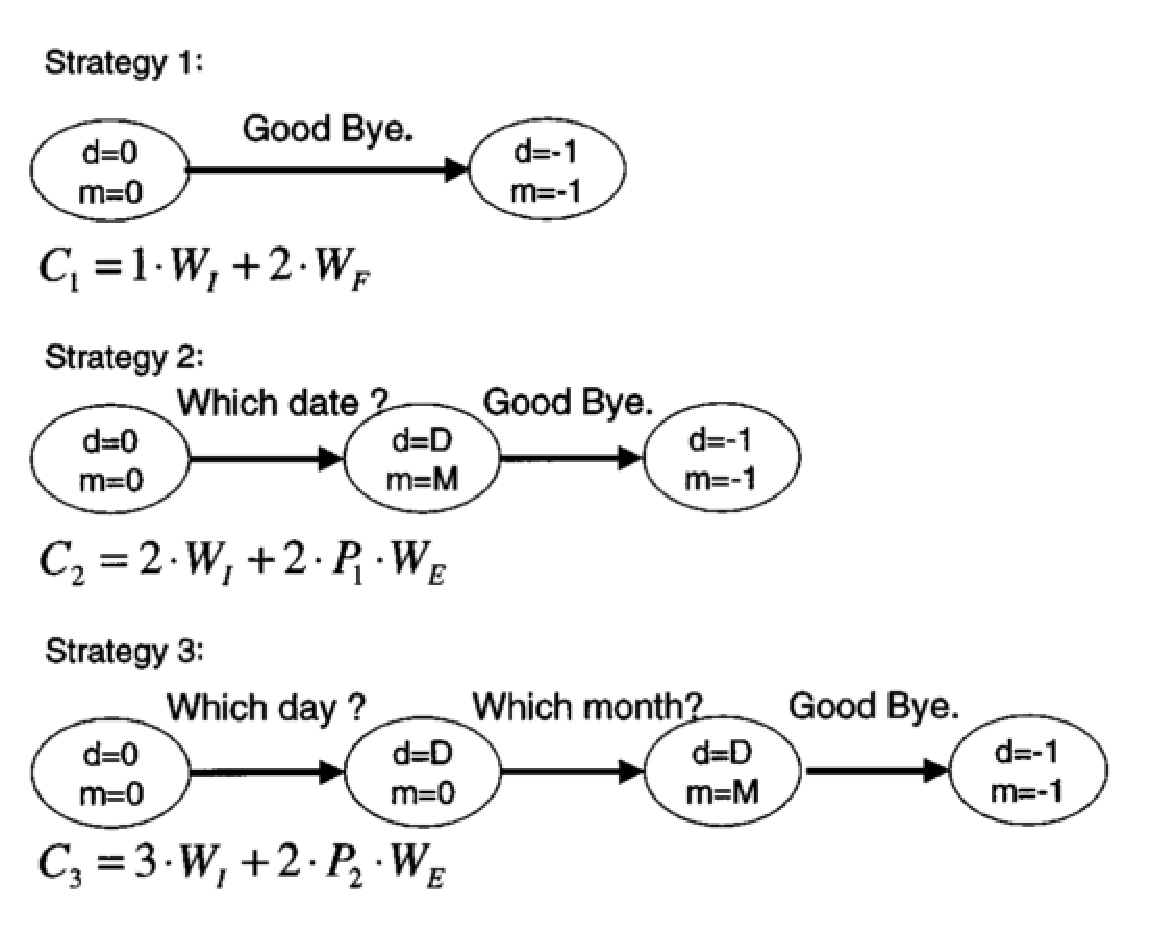
\includegraphics[width=.6\linewidth]{10_17_dialog_MDP1}\\
  \caption{Three possible strategies for the day-month dialog system}\label{fig:dialog_MDP1}
\end{figure}

The next step is to formalize a dialog system as a sequential decision process in terms of its action set, state space, and strategies: 1) The action set of the dialog system includes all possible actions it can perform, such as interactions with the user (e.g., asking the user for input, providing some output, etc.). In the toy example, there are four actions, such as asking for the day $A_d$, asking the month $A_m$, asking the date (day and month) $A_{dm}$, and a final action $A_f$; 2) The state $s$ includes the values of all relevant variables that determine the next action. In the example each state has two integer variables, $d \in \{0, ..., 31\}$ and $m \in \{0, ..., 12\}$, corresponding to the day and month respectively. 3) A dialog strategy maps each state to an action. For example, Figure \ref{fig:dialog_MDP1} shows three possible strategies for the example system.

With some assumptions about the transition probabilities between states, and the cost assignment, the sequential decision process can be formalise as a MDP. Then the optimal strategy can be obtained by a variety of reinforcement learning algorithms.

However, in reinforcement learning, the optimal strategy is learned not from a static corpus but through interaction, because the strategy itself determines the distribution of states in the corpus. To overcome this problem, the paper proposes the use of a \emph{simulated user}. The simulated user is a stochastic generative model that produces speech acts as a response to a dialog action. The simulated user does not deal with the language understanding component - it communicates with the dialog system through semantic representations. The parameters of the simulated user can be estimated from an annotated dialog corpus.

\begin{figure}[htbp]
  \centering
  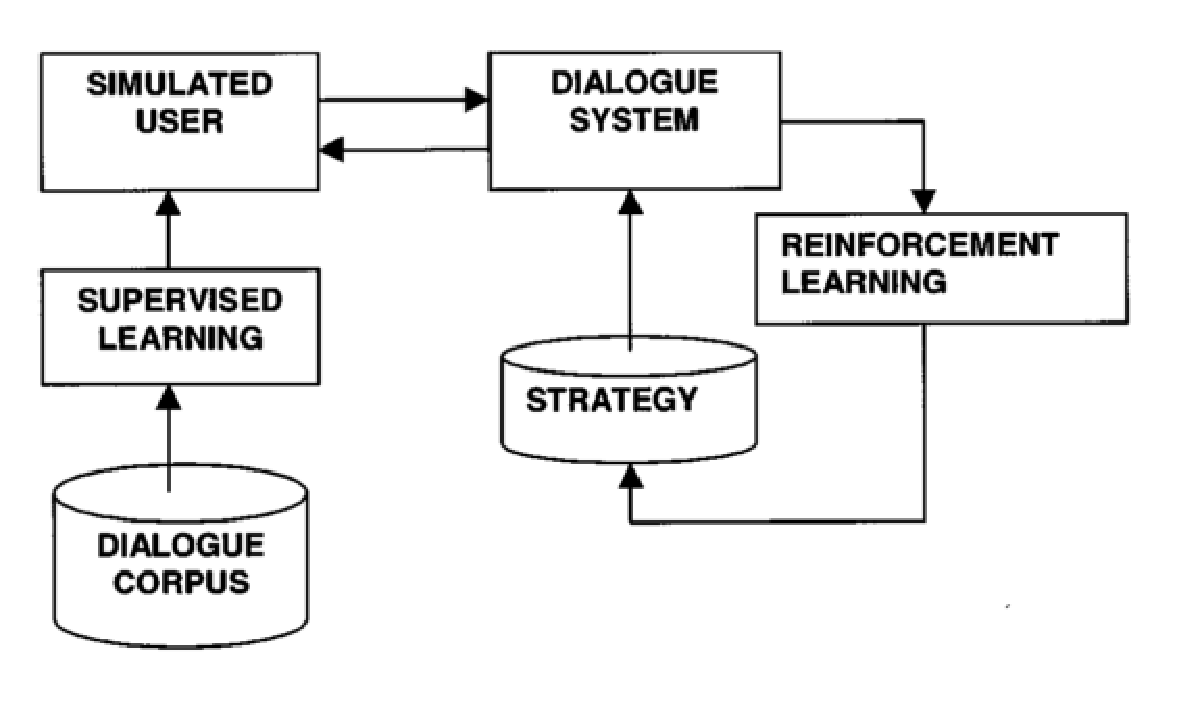
\includegraphics[width=.6\linewidth]{10_17_dialog_MDP2}\\
  \caption{Procedural description of the learning paradigm}\label{fig:dialog_MDP2}
\end{figure}

Once a simulated user is available, it can be used in a generative mode for interacting with the dialog system while the reinforcement learning algorithm is estimating the optimal strategy. Then when a reasonable estimate of the optimal strategy is obtained, the system can be used with real users and the learning process can continue. Figure \ref{fig:dialog_MDP2} summarizes the suggested learning paradigm.

\begin{figure}[htbp]
  \centering
  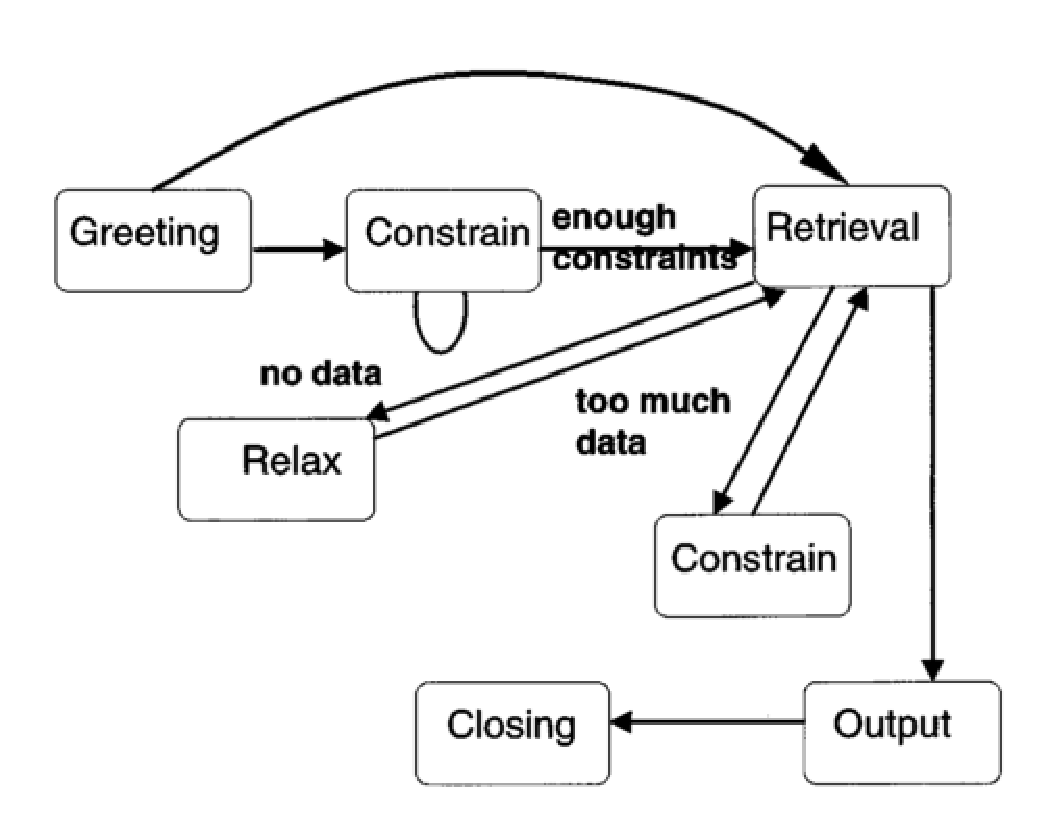
\includegraphics[width=.5\linewidth]{10_17_dialog_MDP3}\\
  \caption{Schematic representation of the optimal strategy for ATIS}\label{fig:dialog_MDP3}
\end{figure}

In the experimental study, the paper shows that a nontrivial strategy can be automatically learned given the simple objective function. For example, Figure \ref{fig:dialog_MDP3} shows the learned strategy of the ATIS task.

Remark: I have also considered formalising the dialog manager as a MDP, and realised one obvious difficulty is that there is not an interactive environment to train the system. This paper introduces simulated users to overcome this difficulty. Another good idea is to abstract the dialog process, such as using semantic representations without considering the ASR or NLU component. I think this paper shows a very promising approach for building our chatbot. 
\subsection{POMDP-based Statistical Spoken Dialogue Systems: a Review \cite{Young2013Pomdp}}

By including an explicit Bayesian model of uncertainty and by optimising the policy via a reward-driven process, \emph{partially observable Markov decision processes (POMDPs)} provide a data-driven framework that reduces the cost of hand-crafting dialog managers and provides robustness against the errors created by speech recognisers operating in noisy environments. This paper provides an overview of the current state of the art in the development of \emph{POMDP-based spoken dialog systems (SDS)}.

\begin{figure}[htbp]
  \centering
  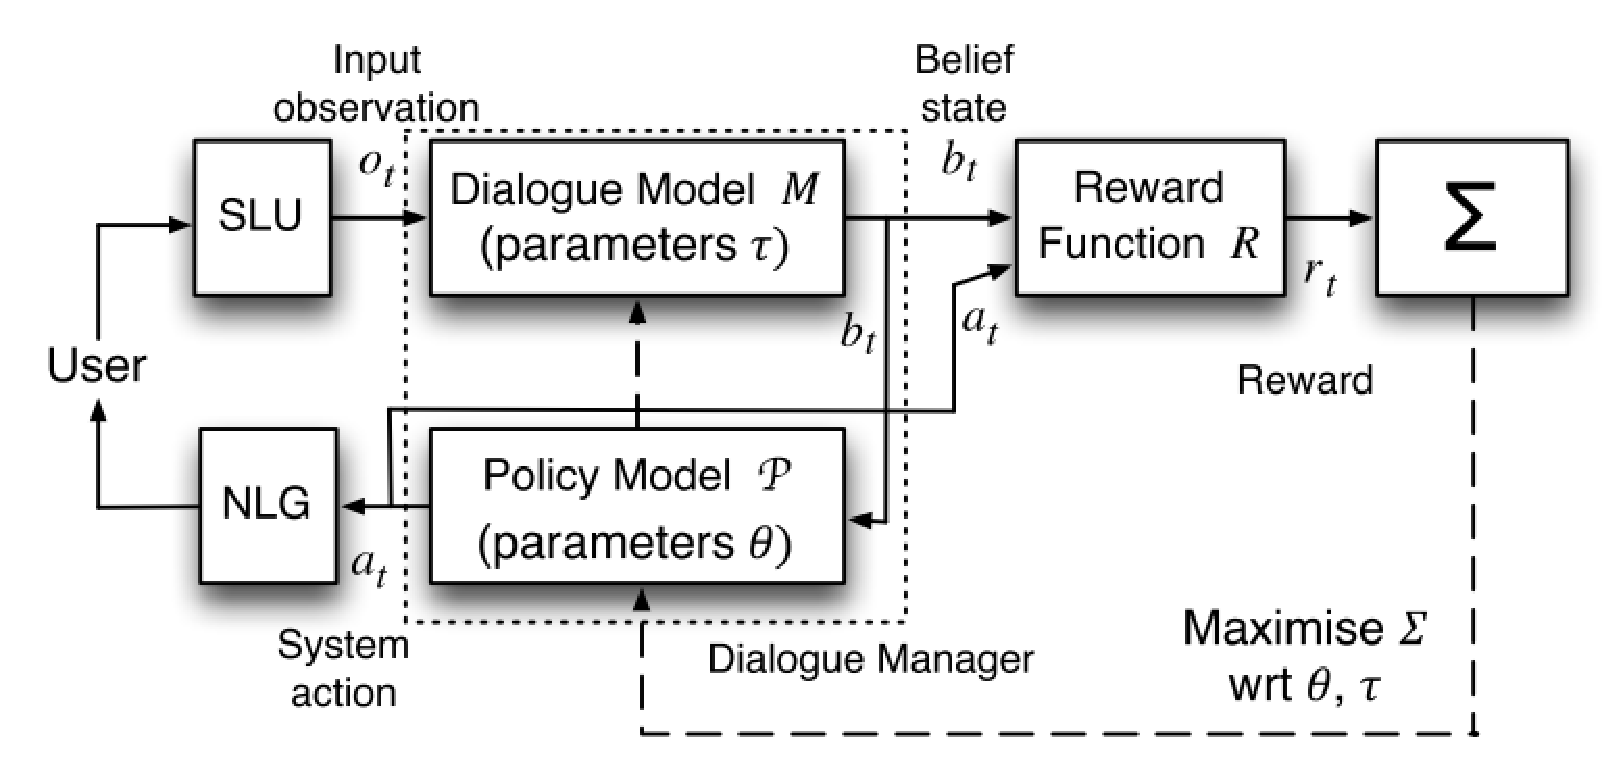
\includegraphics[width=.7\linewidth]{10_17_POMDP1}\\
  \caption{Components of a POMDP-based spoken dialog system}\label{fig:POMDP1}
\end{figure}

%The principal elements of a conventional Spoken Dialog System (SDS) are shown in Figure \ref.
The POMDP approach assumes that dialog evolves as a Markov process, i.e., starting in some initial state, each subsequent state is modelled by a transition probability $p(s_t | s_{t-1}, a_{t-1})$. The state $s_t$ is not directly observable. At each turn, the system regards the output of the SLU as a noisy observation $o_t$ of the user input with probability $p(o_t | s_t)$. The transition and observation probability functions are represented by the dialog model. The decision as to which action to take is represented by the policy. The components of a POMDP-based system are presented in Figure \ref{fig:POMDP1}.

\begin{figure}[htbp]
  \centering
  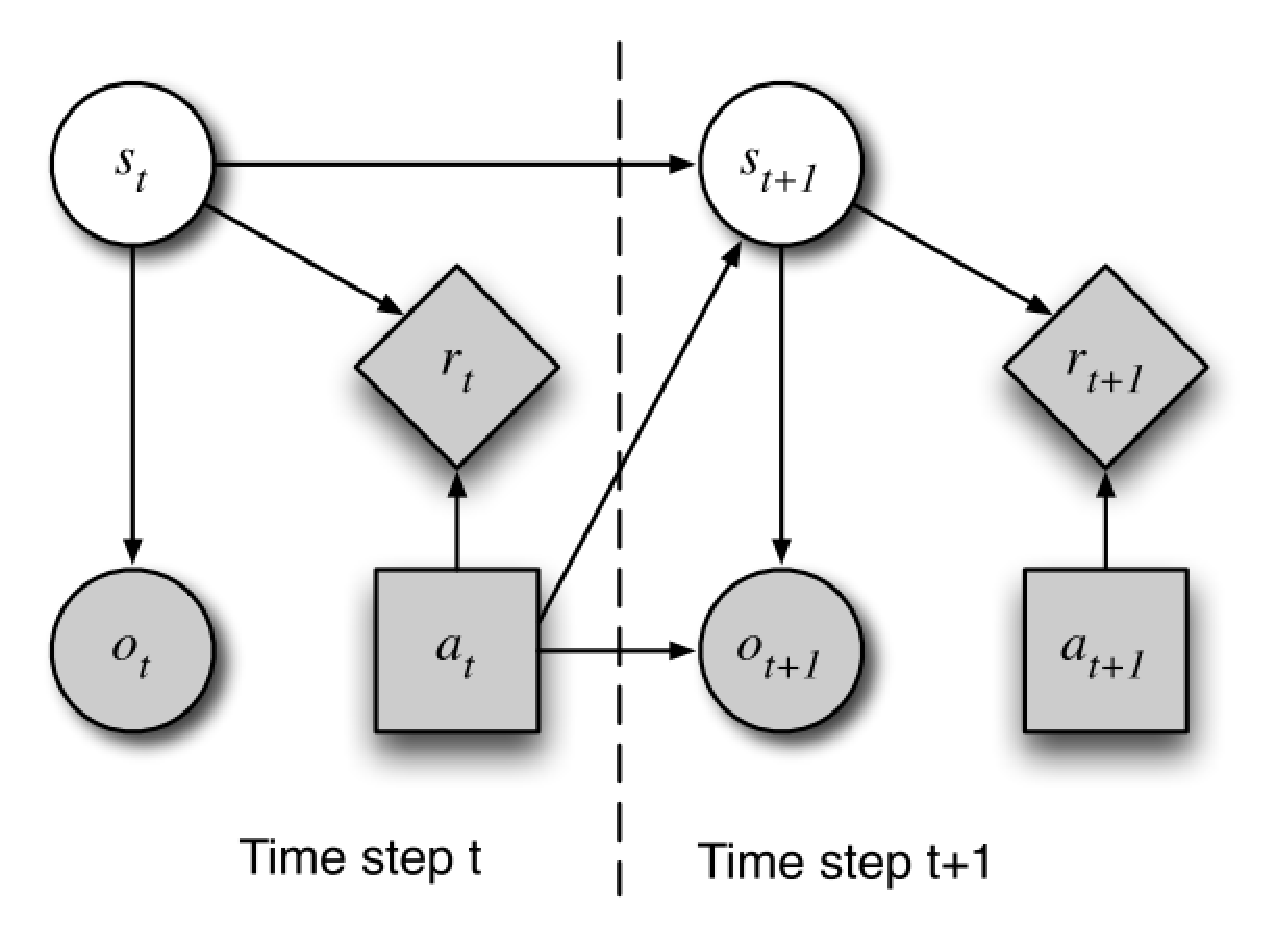
\includegraphics[width=.5\linewidth]{10_17_POMDP2}\\
  \caption{An influence diagram of a POMDP}\label{fig:POMDP2}
\end{figure}

The paper first introduces some preliminary knowledge about the POMDP method. In a POMDP system in each step the world is in some unobserved state $s_t$. Since $s_t$ is not known exactly, a distribution over possible states called a belief state $b_t$ is maintained, where $b_t(s_t)$ indicates the probability of being in a particular state $s_t$. Based on $b_t$, the machine selects an action $a_t$, receives a reward $r_t$, and transitions to (unobserved) state $s_{t+1}$. The machine then receives an observation $o_{t+1}$. This process is represented as an influence diagram in Figure \ref{fig:POMDP2}.

Given an existing belief state $b_t$, the last system action $a_t$, and a new observation $o_{t+1}$, the new updated belief state is given by:
$$b_{t+1}(s_{t+1}) = \eta P(o_{t+1} | s_{t+1}, a_t) \sum_{s_t} P(s_{t+1} | s_t, a_t)  b_t(s_t),$$
where $\eta$ is a normalization constant. The system action is determined by a policy $\pi$. The discounted sum of rewards expected by starting in $b_t$ and following policy $\pi$ is given by the value function $V^\pi(b_t)$. In POMDP, finding an optimal policy is called solving or optimizing the POMDP. However, standard POMDP methods do not scale to the complexity needed to represent a real-world dialog system. So the next sections of this paper introduce some domain-specific methods for applying POMDP in the SDS task.

The first step is to review some possible approaches to represent the dialog model. In a goal-oriented SDS, the state should encode three distinct types of information: the user's goal $g_t$, the intent of the most recent user utterance $u_t$, and the dialog history $h_t$. The resulting influence diagram is shown in Figure \ref{fig:POMDP2}, in which some reasonable independence assumptions have been introduced. Factoring the state in this way can significantly reduce the POMDP model complexity. However, it is still too complex to support tractable real-world systems, so further approximation is necessary. The paper introduces two main approaches: the N-best approach, and the factored Bayesian Network approach.

In N-best approaches, the belief state is approximated by a list of the most likely states with their probabilities. It can also be viewed as running N conventional dialog systems in parallel, such that each parallel thread tracks a different interpretation of what the user said.

\begin{figure}[htbp]
  \centering
  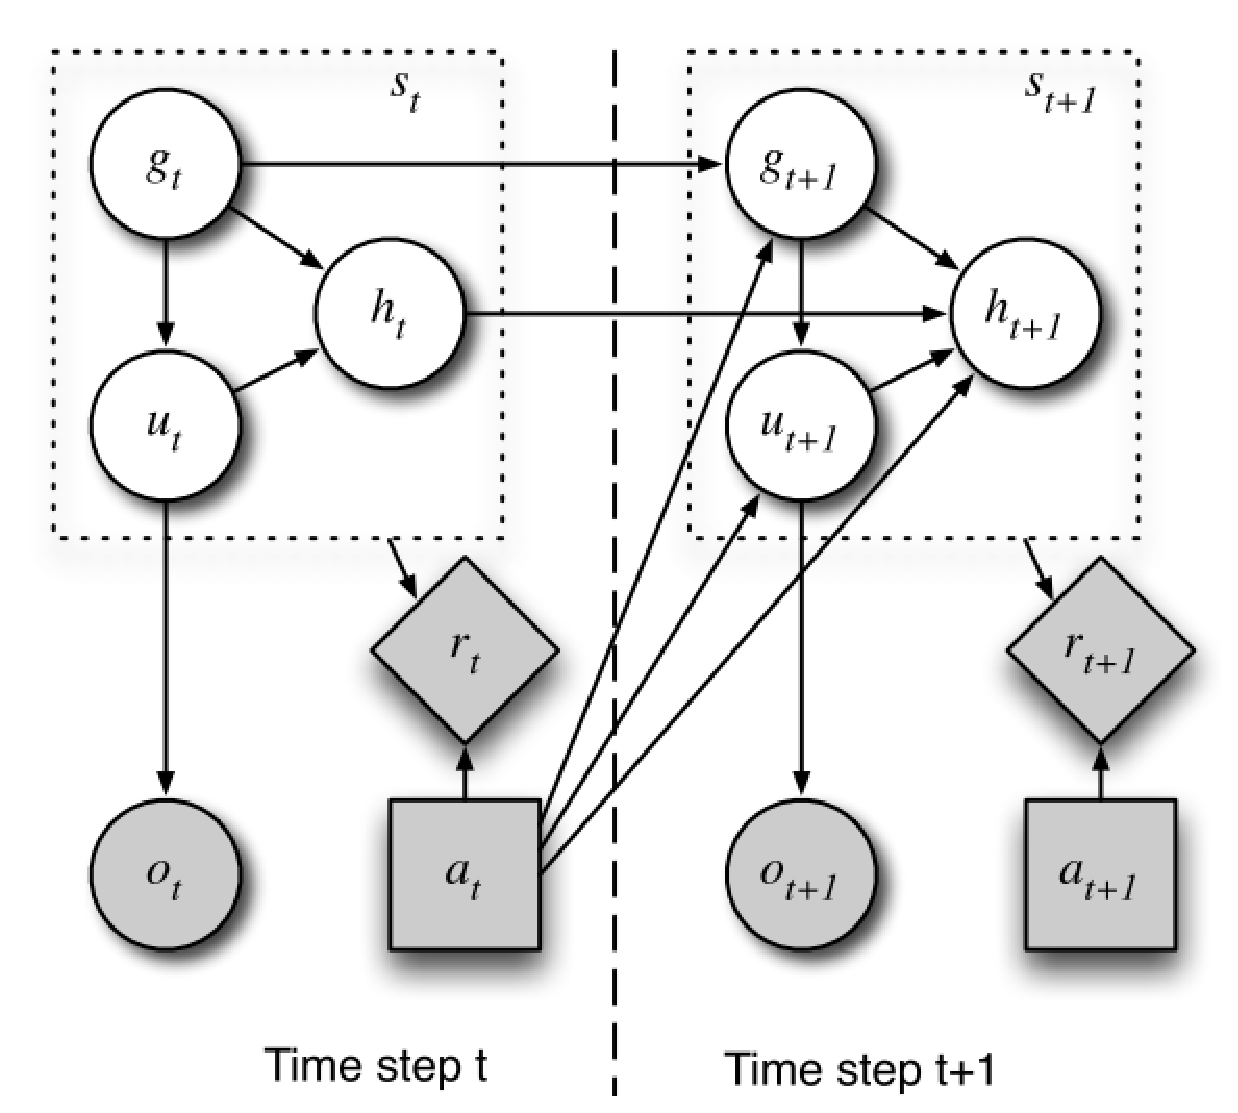
\includegraphics[width=.5\linewidth]{10_17_POMDP3}\\
  \caption{An influence diagram of a factored state POMDP}\label{fig:POMDP3}
\end{figure}

The second approach is to factor the user goal into concepts that can be spoken about by the system. This is illustrated in Figure \ref{fig:POMDP3}, which shows an example from a tourist information system, in which entities have a type, the kind of food served and an area.

The next big challenge of a POMDP-based system is the representation and estimation of the policy model. The paper presents five different methods of policy optimisation: planning under uncertainty, value iteration, Monte-Carlo optimisation, least-squares policy iteration, and natural actor-critic. These methods have been selected because all have been applied to end-to-end working dialog systems.

Another problem is also mentioned in the previous paper summaries of the MDP-based approaches: learning directly from corpora is problematic, because an interactive environment is necessary. One solution is to build a model of the user that can interact directly with a dialog system, and which can itself be trained on corpora. In a real system the dialog manager only has access to a noisy observation, so an error model is needed as well as a user model.

The following three sections presents some more advanced techniques for dialogue model parameter optimisation, fast training, user adaption, and discusses some real-world systems and applications. Finally, the paper discusses the current evaluation methods of SDS. Evaluation of SDS typically falls into one of 3 testing regimes: testing with some form of simulated user, testing with paid subjects, and testing within a live deployed system.

Remark: I am not very familiar with the POMDP approach, so some of the technical details mentioned in the paper are still not very clear to me. Intuitively, POMDP should have better performance than MDP (but also harder to train). I think it is also possible to combine it with the deep learning techniques, such as representing the transition probabilities with a neural network approximately. 
\subsection{On-line policy optimisation of Bayesian spoken dialogue systems via human interaction \cite{Gasic2011}.}

The task is to learn system policy, which determines system acts based on dialouge states (see Table \ref{Goal-Oriented Dialogue System Example} for an example). The paper applies GP-Sarsa to automatic policy learning, which is an online RL algorithms based on Gaussian process \cite{Engel2014Reinforcement}. The GP-Sarsa optimization adopts a more robust filtered reward function \cite{Gasic2011}.

\subsection{A Survey of Statistical User Simulation Techniques for Reinforcement-Learning of Dialogue Management Strategies \cite{Schatzmann2006}}

This paper briefly summarizes the role of the dialogue manager in a \emph{Spoken Dialogue System (SDS)}, gives a short introduction to reinforcement-learning of dialogue management strategies and reviews the literatures on user modelling for simulation-based strategy learning. It further describes recent work on user model evaluation and discusses some of the current research issues.
\begin{figure}[h]
  \centering
  % Requires \usepackage{graphicx}
  \includegraphics[width=.6\linewidth]{khan2004-dm.png}\\
  \caption{learning dialogue strategies with a simulated user}\label{fig:khan04-dm}
\end{figure}

In SDS, the task of the \emph{dialogue Manager (DM)} is to control the flow of the dialogue and to decide which actions to take in response to user input. Specifically, DM needs a \emph{dialogue strategy} that defines when to take the initiative, when to confirm receipt, and so forth. An interesting approach to learn such strategies is through training a statistical, predictive user model for simulating user responses, which can then be used to learn the desired dialogue strategies through trial-and-error interactions (cf. Figure \ref{fig:khan04-dm}).

The second and third sections of the paper discuss  the role of the dialogue management and the reinforcement technique. Since these topics are already covered in other relevant summaries, we choose not to present them here.

Compared with the early rule-based approaches for user modelling, statistical user models are more appealing for the following reasons: 1) The purpose of the user model is not to capture the individual characteristics of a specific user, but to form the basis of a user simulation tool, so it needs to represent the statistical distribution over all types of user behaviour and user responses. These requirements clearly favour a statistical approach; 2) The second advantage of statistical models is that the model parameters can be estimated using real human-computer dialogue data. 3) The user model is also likely to be more robust, more scalable and easier to port to a different domain or dataset. The paper then summaries the recent statistical models into the following groups:

\textbf{N-grams} This method introduces a simple n-gram model for predicting the user action $\hat{a}_{u,t}$ at time $t$ that is most probable given the dialogue history of system and user actions. The weakness of the early bigram model is that it does not place any constraints on the simulated user behaviour. The bigram model is modified to predict only ``sensible'' user responses in some later work, but it still doest not ensure consistency over the course of a dialogue, because of the flawed assumption that every user response depends only on the previous system turn.

\begin{figure}[h]
  \centering
  % Requires \usepackage{graphicx}
  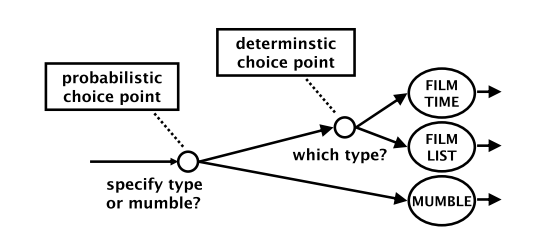
\includegraphics[width=.6\linewidth]{khan2004-graph.png}\\
  \caption{An example of the graph-based approach}\label{fig:khan04-graph}
\end{figure}

\textbf{Graph-based Models} This method combines deterministic rules for goal-dependent actions and probabilistic modelling to cover the conversational behaviour of the simulated user. An example model is shown in Figure \ref{fig:khan04-graph}, in which the arcs of the network represent actions and the nodes represent choice points. Some of the choice points are identified as probabilistic, representing a random decision by the simulated user. The major disadvantage is the high dependence on domain-specific knowledge, and the identification of probabilistic/deterministic choice points requires manual effort.

\begin{figure}[h]
  \centering
  % Requires \usepackage{graphicx}
  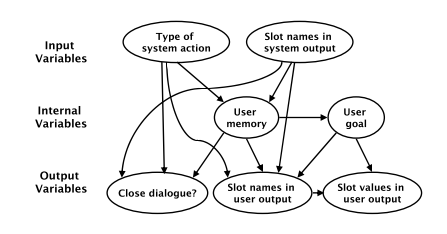
\includegraphics[width=.6\linewidth]{khan2004-bayesian.png}\\
  \caption{An example of the Bayesian Network approach}\label{fig:khan04-bayesian}
\end{figure}


\textbf{Bayesian Networks} The goal of this approach is to avoid the manual effort involved in building networks of choice points, while ensuring that actions are consistent with the user's goal. Figure \ref{fig:khan04-bayesian} shows an example of the network. It is suggested that the network can be easily extended to include factors such as the level of cooperativeness, the degree of initiative, etc.

\textbf{Machine-Learning Techniques} Recent work by Georgila et al. \cite{Georgila2005} returns to Markov models and explores the use of richer state descriptions, longer dialogue histories and machine-learning techniques. They use linear feature combination to map from a state $s$ to a vector of real-valued features $f(s)$. Supervised learning is then used to estimate a set of weights which describe how useful each vector element of $f(s)$ is for predicting an action $a$.

\begin{figure}[h]
  \centering
  % Requires \usepackage{graphicx}
  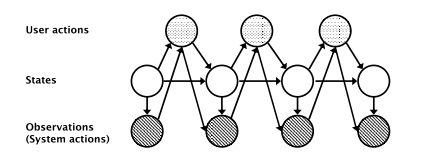
\includegraphics[width=.6\linewidth]{khan2004-hmm.png}\\
  \caption{An example of the HMM approach}\label{fig:khan04-hmm}
\end{figure}

\textbf{Hidden Markov Models} In the work of \cite{Cuayahuitl2005}, the authors experiment with different variations of HMMs, and show that the most advanced one is an \emph{Input-Output-HMM (IOHMM)}  (cf. Figure \ref{fig:khan04-hmm}). The behaviour of the model is governed by a set of transition probabilities $P(q_{t+1} | q_t, a_{u,t})$ and a set of output probabilities $P(a_{s,t} | q_t, a_{u, t-1})$. User responses are predicted using $P(a_{u,t} | q_t, a_{s,t})$.

Finally the paper introduces some evaluation techniques, in which a distinction can be made between \emph{direct} methods and \emph{indirect} methods. Direct evaluation methods assess the user model by testing the quality of its predictions, such as accuracy, precision and recall. Indirect evaluation metrics such as utility attempt to measure the quality by evaluating the effect on the system performance.

\subsection{End-to-end LSTM-based dialog control optimized with supervised and reinforcement learning \cite{Williams2016End}}

The paper presents a model for end-to-end training of goal-oriented dialogue systems, which breaks the operational loop of a dialogue system down into 13 steps (Figure \ref{fig:Williams2016End01}). The model combines recurrent neural networks and domain-specific software that expresses business rules and provides API access in the domain. The recurrent neural networks automatically infer dialogue state representation, and thus hand-coded state features are not needed.

\begin{figure}[htbp]
  \centering
  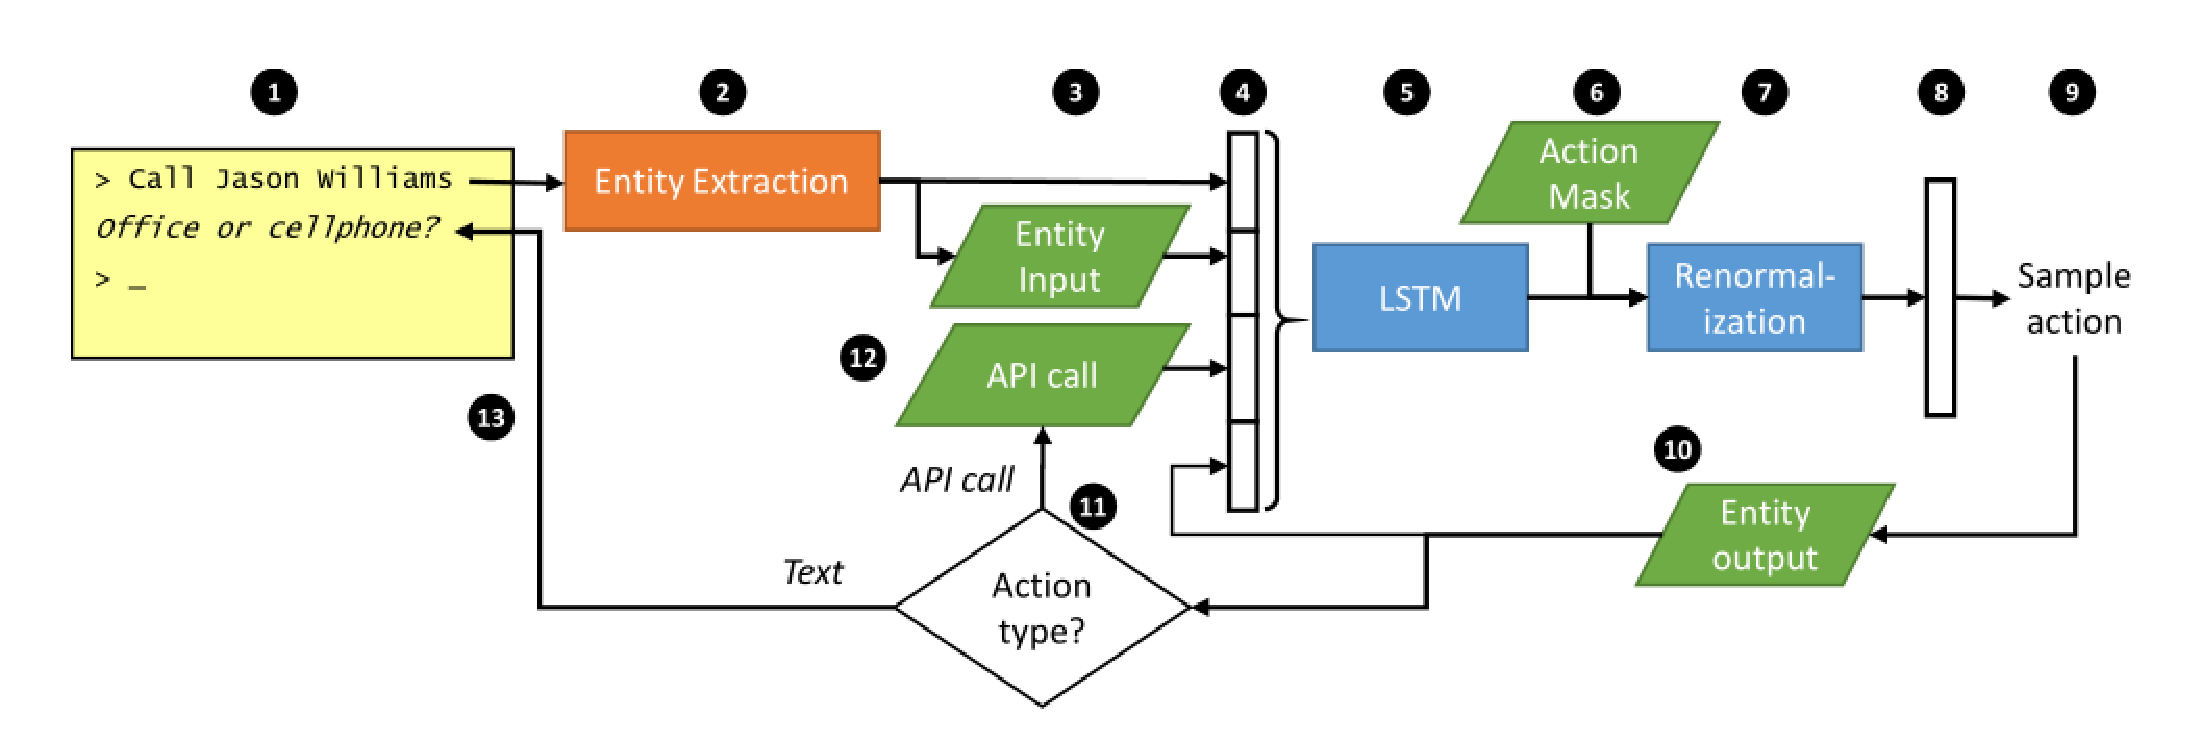
\includegraphics[width=\linewidth]{Williams2016End01}\\
  \caption{Operational loop of a dialogue system}\label{fig:Williams2016End01}
\end{figure}

The operational cycle has 13 steps: (1) The system receives user input; (2) The entities mentioned in user input are identified; (3) The extracted entities are resolved into ground entities corresponding to one or more rows in a database; (4) A feature vector is constructed from four sources; (5) LSTM takes the feature vector, update its hidden states, and outputs a distribution over all template actions; (6) Domain-specific software provides an action mask indicating actions that are not allowed at the current time; (7, 8) The task mask is combined with the distribution in step five into a new distribution; (9) An action is chosen from the new distribution; (10) The selected template action is instantiated with the entities in step three; (11, 12, 13) Depending on the action type, the system either invokes the corresponding API call or render the response text to users. 
\subsection{Learning End-to-End Goal-Oriented Dialog \cite{Bordes2016Learning}}

The main contributions of the paper are: (1) propose to evaluate end-to-end dialogue systems using goal-oriented tasks, and design five tasks in the application of restaurant reservation; (2) apply Memory Networks to train an end-to-end dialogue system, and show that per-response performance is encouraging.

The five tasks are (1) issue API calls. The system should ask questions, gather information about the preferred cuisine type, location, price range, and party size of restaurants, and generate the correct API call; (2) update API calls. When user preferences change, the system should update the API call; (3) display options. The system should propose the restaurants, which match user preferences, until users accept; (4) provide extra information. When users ask for the phone numbers and address of a restaurant, the system should answer correctly based on the facts; (5) conduct full dialogues (see Figure \ref{fig:Bordes2016Learning01} for examples of the five tasks). Natural language patterns and knowledge base entities are combined to generate simulated dialogues consisting of user and system utterances.

\begin{figure}[htbp]
  \centering
  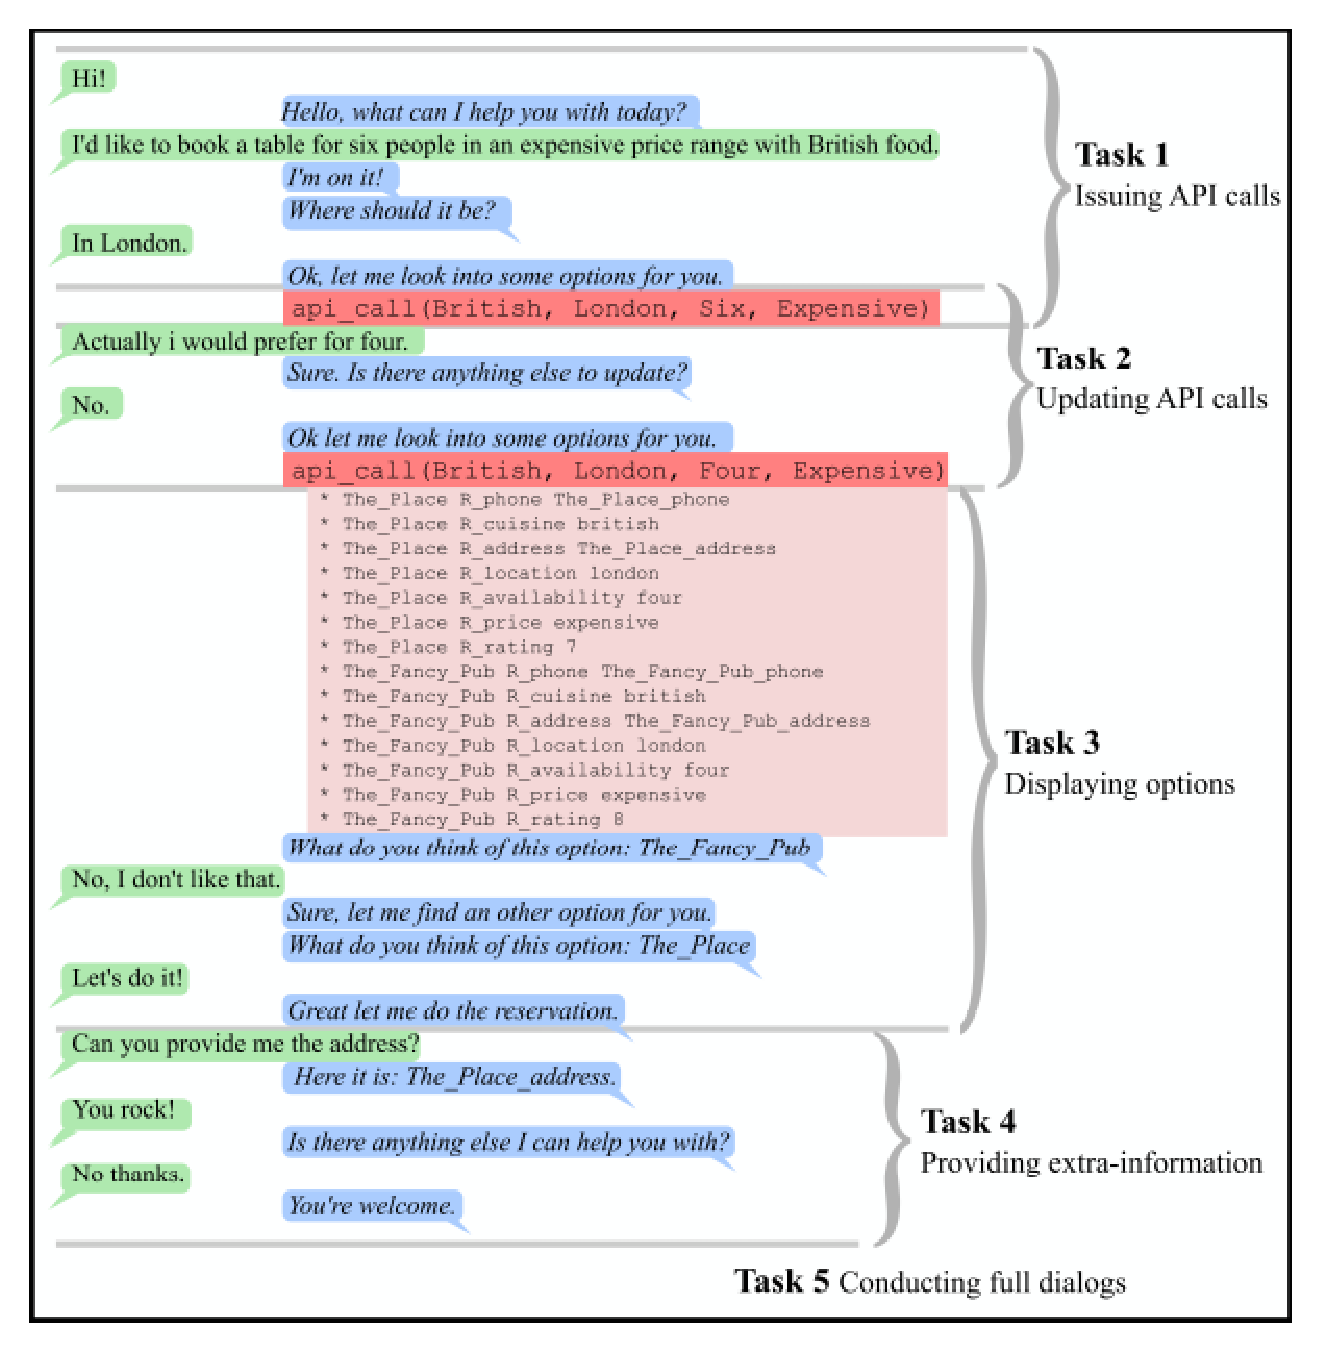
\includegraphics[width=.8\linewidth]{Bordes2016Learning01}\\
  \caption{Examples of the five tasks}\label{fig:Bordes2016Learning01}
\end{figure}

The paper uses a retrieval-based method, i.e. selecting the best candidate response from a large set of all possible system utterances and API calls. The paper applies Memory Networks that consist of three component (1) store conversation in memory; (2) read pertinent information from the memory; (3) use the information to output the best candidate response. 
\subsection{A Network-based End-to-End Trainable Task-oriented Dialogue System \cite{Wen2016}}
The task is to help humans find a desired restaurant and the contact information from a database by conversing naturally with them. The paper proposes an end-to-end trainable framework for task-oriented systems shown in Figure \ref{fig:Wen2016Network01}.

\begin{figure}[htbp]
  \centering
  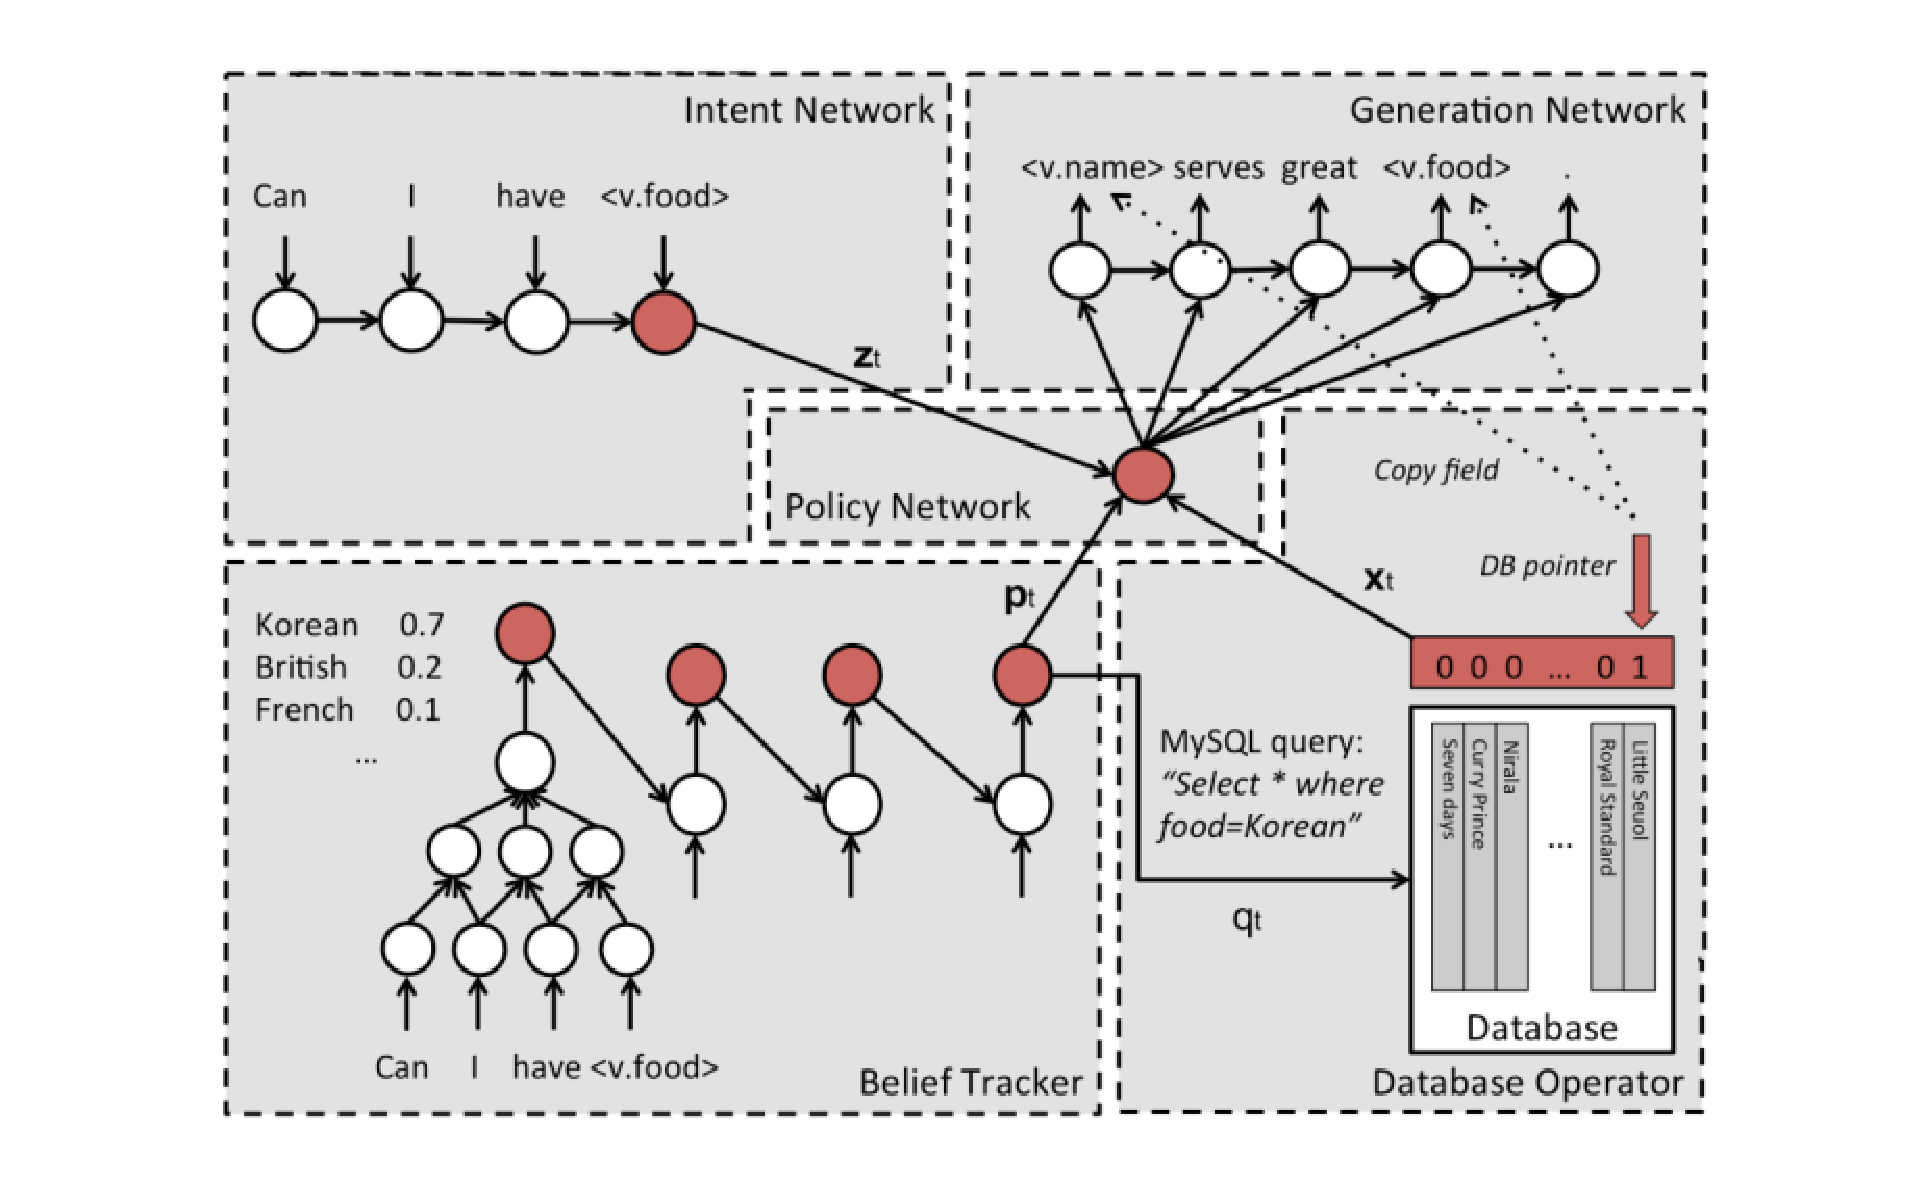
\includegraphics[width=0.9\linewidth]{Wen2016Network01}
  \caption{An end-to-end trainable framework for task-oriented systems}
	\label{fig:Wen2016Network01}
\end{figure}

At each turn, the system takes an user utterance $u^{t}$ as input, which is used to update two internal representations by an intent network and a set of belief trackers: (1) A distributed representation; (2) A distribution over the values, belief state, for each slot. The database operator uses the most likely values in the belief state, and returns the matched restaurants in the database. The policy network combines the distributed representation, belief state, and search results to form an action vector representing the next action. Conditioned on the action vector, the generation network produces template-like sentences whose generic tokens are then replaced by the actual values. Each components are described in more detail below:

\begin{itemize}
\item[-] \textbf{Intent Network} encodes $u^{t}=w^{t}_{0}, ..., w^{t}_{N}$ into a distributed representation $z^{t}$ at turn $t$. a LSTM is used and the last hidden state $z^{t}_{N}$ is taken as the distributed representation:
\begin{equation}
z^{t} \ = \ z^{t}_{N} \ = \ LSTM( w^{t}_{0}, ..., w^{t}_{N} )
\end{equation}

\item[-] \textbf{Belief Trackers} maintain a multinomial distribution $p^{t}_{s}$ for each informable slot and a bernoulli distribution $p^{t}_{s}$ for each requestable slot. The distributions are updated by:
\begin{equation}
\begin{aligned}
f^{t}_{s}(v) \ =& \ f^{t}_{s}(v,cnn) \oplus p^{t-1}_{s}(v) \oplus p^{t-1}_{s}(\emptyset) \\
g^{t}_{s}(v) \ =& \ U_{s} sigmoid( W_{s}f^{t}_{s}(v) + B_{s} ) + D_{s} \\
p^{t}_{s}(v) \ =& \ \frac{\exp(g^{t}_{s}(v))}{\exp(g^{t}_{s}(\emptyset)) + \sum_{v} \exp(g^{t}_{s}(v))} \\
\end{aligned}
\end{equation}
where $f^{t}_{s}(v)$ is the concatenation of two CNN feature vectors, one from processing $u^{t}$ and the other from processing the last action $a^{t-1}$.

\item[-] \textbf{Database Operator} forms a query
\begin{equation}
q^{t} \ = \ \cup_{s} { argmax_{v} p^{t}_{s}(v) }
\end{equation}
and create a binary vector $x^{t}$ over the restaurants in the database where a 1 means that the corresponding restaurant is consistent with the query.

\item[-] \textbf{Policy Network} outputs an action vector $o^{t}$ by:
\begin{equation}
o^{t} \ = \ \tanh( W_{z} z^{t} + W_{p} \oplus_{s} \hat{p}^{t}_{s} + W_{x} \hat{x}^{t} )
\end{equation}
where $\hat{p}^{t}_{s}$ is the belief summary consisting of (1) the summed value probabilities; (2) the probability that the user do not care; (3) the probability that the slot has not been mentioned, and $\hat{x}^{t}$ is a 6-bin 1-hot encoding vector based on the number of matched restaurants in $x^{t}$.

\item[-] \textbf{Generation Network} generates templates token by token conditioned on the action vector:
\begin{equation}
P(w^{t}_{i+1} | w^{t}_{i}, h^{t}_{i-1}, o^{t}) \ = \ LSTM( w^{t}_{i}, h^{t}_{i-1}, o^{t} )
\end{equation}
Instead of conditioning on a single action vector $o^{t}$, an attention mechanism can also be used to produce templates.

\end{itemize}
\subsection{Word-based dialog state tracking with recurrent neural networks \cite{Henderson2014Word}}

The task is to converts user inputs into dialogue states (see Table \ref{Goal-Oriented Dialogue System Example} for an example of dialogue state). The dialogue state is a probability distribution over handcrafted goals, methods, and requested slots. The paper uses a RNN to compute the distribution over goal values for each goal, a RNN to compute the distribution over methods, and a RNN to compute the distribution over requested slots. During training, gradient clipping is used to avoid exploding gradients \cite{Pascanu2012Understanding}.

\begin{table}[!hbp]
\begin{tabular}{|r|rl|}
\hline
\textbf{System Output} & \multicolumn{2}{l|}{You can ask for restaurants by area, price range or food type.} \\
\hline
\textbf{User Input} & \multicolumn{2}{l|}{Expensive restaurant in the south part of town.} \\
\hline
\emph{Dialogue State} & goals
& 0.7 pricerange=expensive area=south \\
&& 0.2 pricerange=expensive area=north \\
& methods & 0.9 method=byconstraints \\
&& 0.1 method=byalternatives \\
& requested slots & 0.0 address \\
&& 0.0 phone \\
\hline
\emph{System Act} & \multicolumn{2}{l|}{request(food)} \\
\hline
\textbf{System Output} & \multicolumn{2}{l|}{What kind of food would you like?} \\
\hline
\end{tabular}
\caption{Goal-Driven Dialogue System} \label{Goal-Oriented Dialogue System Example}
\end{table}
\subsection{End-to-End Reinforcement Learning of Dialogue Agents for Information Access \cite{Dhingra2016End}}
The task is to provide a user with an sorted list of entities, which are believed to match the user goal, from a database through dialogue. The paper presents an end-to-end trainable system: \emph{KB-InfoBot}. The high-level overview of KB-InfoBot is shown in Figure \ref{fig:Dhingra2016End01}.

\begin{figure}[htbp]
  \centering
  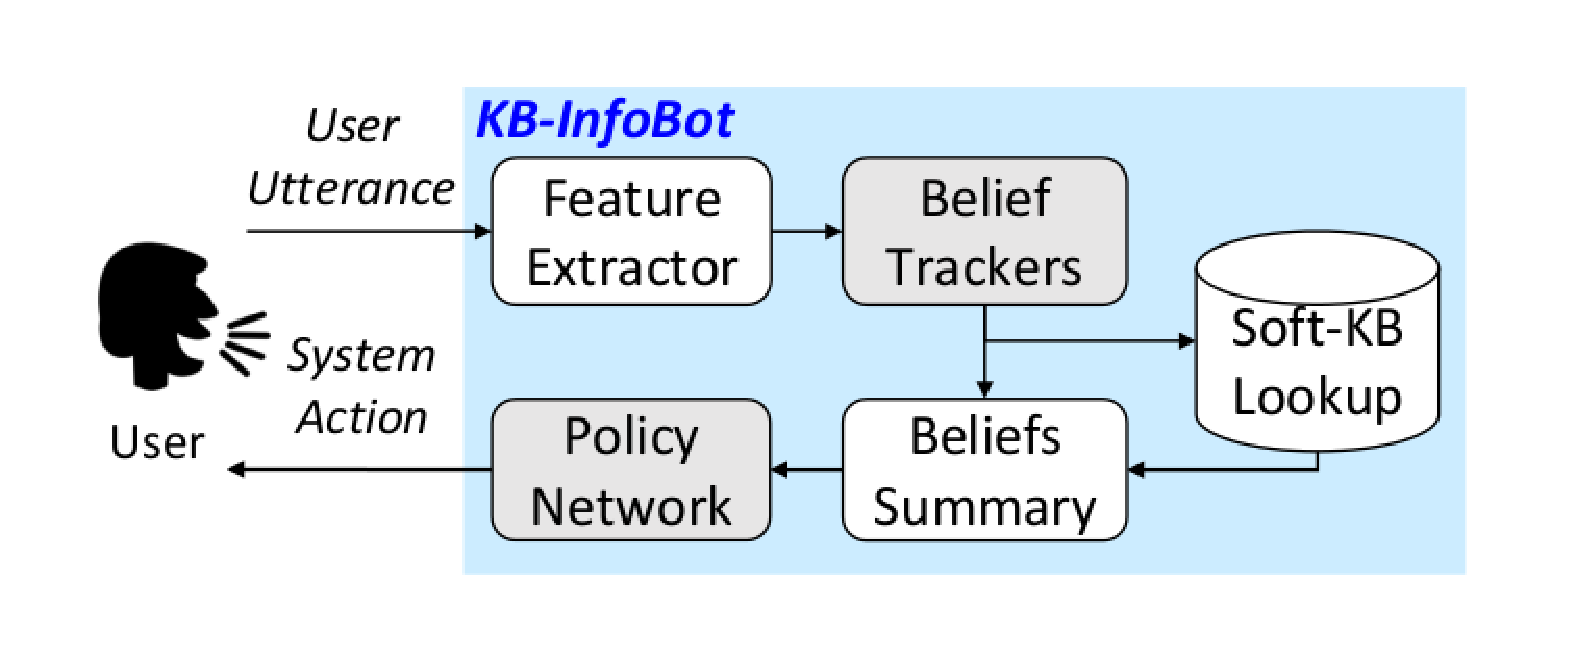
\includegraphics[width=0.8\linewidth]{Dhingra2016End01}
  \caption{KB-InfoBot}
	\label{fig:Dhingra2016End01}
\end{figure}

Assuming that in the database, there are $N$ entities, each of which has $M$ slots. At each turn, the input is an user utterance $u^{t}$ and the output is a system action $a^{t}$. The action space $\mathcal{A}$ has $M+1$ actions: (1) \emph{request($s_{j}$)} asking the user for the value of slot $j$ for $1 \leq j \leq M$; (2) \emph{inform($I$)} showing an sorted list of entities to the user. Each component of KB-InfoBot is defined as follows:

\begin{itemize}
\item[-] \textbf{Feature Extractor} converts $u^{t}$ into a vector representation $x^{t}$, each element of which indicates the count of a certain 2-gram in $u^{t}$. The vocabulary size is 3078 and thus $x^{t}$ is a 3078-dimensional vector.

\item[-] \textbf{Belief Tracker} takes $x^{t}$ as input and for each slot, updates the internal representation $h^{t}_{j}$ and outputs the belief state $p^{t}_{j}$ and $q^{t}_{j}$. The internal representation starting from $h^{0}_{j}=\mathbf{0}$ is updated by a Gated Recurrent Unit:
\begin{equation}
\begin{aligned}
r^{t}_{j} \ =& \ \sigma( W^{r}_{j}x^{t} + U^{r}_{j}h^{t-1}_{j} + b^{r} ) \\
z^{t}_{j} \ =& \ \sigma( W^{z}_{j}x^{t} + U^{z}_{j}h^{t-1}_{j} + b^{z} ) \\
h^{t}_{j} \ =& \ (1-z^{t}_{j}) \odot h^{t-1}_{j} + z^{t}_{j} \odot \tanh( W^{h}_{j}x^{t} + U^{h}_{j}(r^{t}_{j} \odot h^{t-1}_{j}) + b^{h} ) \\
\end{aligned}
\end{equation}
Then, the belief state is computed:
\begin{equation}
\begin{aligned}
p^{t}_{j} \ =& \ softmax( W^{p}_{j}h^{t}_{j} + b^{p}_{j} ) \\
q^{t}_{j} \ =& \ \sigma( W^{q}_{j}h^{t}_{j} + b^{q}_{j} ) \\
\end{aligned}
\end{equation}
where $p^{t}_{j}$ is a multinomial distribution over all the possible values of slot $j$, and $q^{t}_{j}$ is a bernoulli distribution indicating whether the user know the value of slot $j$ or not.

\item[-] \textbf{Soft-KB Lookup} uses $p^{t}_{j}$ and $q^{t}_{j}$ to compute $p^{t}$, the posterior distribution over the entities in the database:
\begin{equation}
p^{t}(i) \ \propto \ \prod_{j=1}^{M} p^{t}_{j} (i) \\
\end{equation}
which is the posterior probability that the $i$th entity is targeted by the user.
\[
    p^{t}_{j}(i) \ = \
\begin{cases}
    \frac{1}{N},                                                                                     & \text{if } i \in M_{j} \\
    q^{t}_{j}\frac{p^{t}_{j}(i_{j})}{N_{j}(i_{j})} (1- \frac{|M_{j}|}{N}) + (1-q^{t}_{j})\frac{1}{N},& \text{otherwise}
\end{cases}
\]
where $N_{j}(i_{j})$ is the count of value $i_{j}$ in slot $j$, and $M_{j}$ is the set of entities for which the value of slot $j$ is missing.

\item[-] \textbf{Beliefs Summary} summarizes slot $j$ into an entropy statistic, $H(p^{t}_{j})$, over a distribution $w^{t}_{j}$:
\begin{equation}
w^{t}_{j}(v) \ \propto \ \sum_{i:i_{j}=v} p^{t}(i) + p^{0}_{j}(v) \sum_{i:i_{j}\ is\ missing} p^{t}(i) \\
\end{equation}
In a similar way, $p^{t}$ is summarized into $H(p^{t})$. The summary vector $s^{t}=[H(p^{t}_{1}), ..., H(p^{t}_{M}), q^{t}_{1}, ..., q^{t}_{M}, H(p^{t})]$ is input to the policy network.

\item[-] \textbf{Policy Network} selects the next action based on the dialogue history and the current summary vector $s^{t}$:
\begin{equation}
\begin{aligned}
h^{t}_{\pi} \ =& \ GRU( s^{1}, ..., s^{t} ) \\
\pi \ =& \ softmax( W^{\pi}h^{t}_{\pi} + b^{\pi} ) \\
\end{aligned}
\end{equation}

\item[-] \textbf{Action Selection} samples the next action from the polity $\pi$. If action \emph{inform()} is chosen, an ordered list $I=(i_{1}, ..., i_{R})$ of indices is provided to the user.
\end{itemize}

\section{Natural Language Generation}

The generation component of a conversational agent chooses the concepts to express to the user, plans out how to express these concepts in words, and assigns any necessary prosody to the words \cite{Jurafsky2006}. In other words, the NLG component generates surface texts based on abstract system actions \cite{Wen2015a}.

We begin with introducing the idea of Wilcock and Jokinen about what should be a good generation models for spoken dialogue systems \cite{wilcock2003}. Many early SDS systems use simple template or grammar methods for generation. In order to made the responses more diverse, statistical-based methods are also introduced \cite{Oh2000}.

One of the most recent important technique in the field of natural langue processing is the word-embedding technique, which learns a distributed representation of each word. In this section, we begin with introducing one of the classic paper of the word-embedding techniques \cite{Bengio2003A}. The next several papers \cite{Wen2015Stochastic, Martens2011, Mikolov2010} show how the new emerged deep learning methods, particularly the recurrent neural networks, are applied in the NLG component.
 
Another kind of language model is based on the (restricted) Boltzmann machine. We introduce the mathematical background of RBM \cite{Bengio2009}, and then present a paper that successfully exploits this technique \cite{Mnih2007}. %Several other DNN based language models will also be presented \cite{Mnih2007}.

\subsection{Generation Models for Spoken Dialogues \cite{wilcock2003}}

This paper discusses what kind of \emph{generation model} is suitable for spoken dialogue responses, by considering different aspects of the generation component for a spoken dialogue system. It argues that the flexibility needed in spoken dialogue systems can be addressed by a suitable generation model.

The paper begins with a comparison of different existing generation methods: the \emph{machine translation model}, the \emph{text generation model}, and a \emph{template model} used for telephone booking.

In machine translation, the source information is generally viewed as unordered. When this form of bag generation is used for dialogue response generation, the problem is that the information structure, i.e. which information is new and important than the others, is not taken into account as a significant factor during the generation.

In the model of generation adopted in text generation systems, information structure is recognised as a major factor. This model usually has a pipeline architecture, ensuring that topic shifts and old and new information status are properly handled. However, it is designed for producing text which is basically monologue, which is essentially a one-shot process. In spoken interaction, part of the relevant information can be given initially, and the rest can be given later depending on the user's reactions to the first part. So this model is also not suitable for generation in a spoken dialogue system.

Another model of generation, developed for telephone-based booking and ordering systems, is based on the use of dialogue description languages, such as VoiceXML. This model, however, suffers from the disadvantage that it tends to increase the rigidity of the system, by enforcing a form-filling approach which makes the user fit in with the system's demands. Furthermore, information-providing systems often encounter situations where they need to present large amounts of complex information to the user, and need to present this in a way that is accessible and clear. Consequently, dialogue systems should also have more sophisticated models for generation.

The paper then describes the model of generation which the authors advocate for spoken dialogue systems. It is argued that an agenda type of interface is suitable for spoken dialogue systems, in which new information status is already marked up by the dialogue manager.

The model proposed in this paper is called NewInfo-based model. The key idea is that the generator decides how to present new information to the user: whether to present it by itself, or wrap it in appropriate linking information. The choice of wrapping or not depends on the changing dialogue context. When the communication channel is working well, wrapping can be reduced, but when there are uncertainties about what was actually said, wrapping must be increased to provide implicit confirmation.

In this approach, the dialogue manager creates an \emph{Agenda}, which is a set of domain concepts available for use by the generator. The generator can freely use the concepts to realise the system's intention as a surface string, but it is not force to include all the concepts in the response. Since the dialogue manager is responsible for recording dialogue history, it is the best authority to decide the new or old information status of each concept.

Finally, the paper demonstrates the approach with an implemented system. The working system supports incrementality, immediacy and interactivity due to the underlying generation model. It supports the argument that the flexibility needed in spoken dialogue systems can be addressed by a suitable generation model.

\subsection{Stochastic Language Generation for Spoken Dialogue Systems \cite{Oh2000}}

This paper proposes a new corpus-based approach to natural language generation, specifically designed for \emph{\emph{Spoken Dialogue Systems (SDSs)}}. This work is motivated by the observation that the two current approaches to language generation, \emph{template-based} and \emph{rule-based} NLG have limitations when applied to SDSs.

The basic idea of this paper is to develop a corpus-based generation system, in which it models language spoken by domain experts performing the task of interest, and uses that model to stochastically generate system utterance. It used two corpora in the travel reservations domain. One corpus consists of 39 dialogues, and another corpus consists of 68 dialogues.

\begin{figure}[h]
  \centering
  % Requires \usepackage{graphicx}
  \includegraphics[width=.6\linewidth]{Oh00-NLG_overall_arch.png}\\
  \caption{Overall architecture.}\label{fig:Oh00-NLG_overall_arch}
\end{figure}

The overall architecture of the NLG system is shown in Figure \ref{fig:Oh00-NLG_overall_arch}. The \emph{content planning} components decides which attributes should be included in an utterance, and the \emph{surface realization} component decides how to translate the attributes to natural language. Next we will introduce these two components in more details.

The paper presents two approaches for content planning. The first approach, called \emph{old versus new}, selects only new information to be included in the system utterance. The second approach is to use a statistical model. The model first predicts the number of attributes in the system utterance, by learning the probability distribution $P(n_k) = P(n_k | c_k)$, where $n_k$ is the number of attributes and $c_k$ is the utterance class for system utterance $k$. The second step of the model is to select the attributes by
$$A^* = \mathop{\arg \max}_{a_1, ..., a_n} \sum_{k=1}^m P(b_k) \prod_{i=1}^n P(a_i | b_k),$$
where $\{b_1, ..., b_m\}$ is the set of $m$ attributes in the preceding user utterance.

The stochastic surface realization component uses different levels of generation granularity to various utterance classes. For example the hello message can be simply generated by a fixed expression, while the more complex output is generated by a statistical language model. There are four aspects of the surface realizer which will be discussed in what follows: building language models, generating candidate utterances, scoring the utterances, and filling in the slots.

When building the language model, the system first replaces tokens by their word classes (e.g. ``U.S. Airways'' by ``airline''). Then it uses a 5-gram model to introduce some variability in the output utterances while preventing nonsense responses.

The input to NLG from the dialogue manager is a frame of attribute-values pairs. The generation engine uses the appropriate language model for the utterance class and generates word sequences randomly according to the language model distributions.

For each randomly generated utterance, it computes a penalty score. The score is based on the heuristics that are empirically selected. The generation engine generates a candidate utterance, scores it, keeping only the best-scored utterance. It stops and returns the best utterance when it finds an utterance with a zero penalty score, or runs out of time.

The last step is filling slots with the appropriate values. For example, the utterance ``What time would you like to leave \{depart\_city\}?'' becomes ``What time would you like to leave New York?''.

In the experimental study, the paper conducts a comparative evaluation by running two identical systems varying only the generation component. Twelves subjects were involved in the experiment. It is shown that the subjects prefer the new versus old content planning approach, and the stochastic generation model. However, both the results are not statistically significant. The authors were still in the process of designing a larger evaluation.

\subsection{A Neural Probabilistic Language Model \cite{Bengio2003A}}

This paper proposes a neural network architecture to learn a probabilistic language model. The method can simultaneously learn a distributed representation for each word and the probability function for word sequences.

A goal of statistical language modeling is to learn the joint probability function of sequences of words in a language. It can be represented by the conditional probability of the next word given all the previous ones:
$$P(w_1^T) = \prod_{i=1}^T P(w_t | w_1^{t-1}).$$
Here $w_t$ is  the $t$-th word, and $w_i^j = (w_i, w_{i+1},... , w_j)$ is the subsequence from the $i$-th to the $j$-th word.

One of the motivations of this paper is that traditional $n$-gram models do not take into account of the similarity between words. For example, having seen the sentence ``The cat is walking in the bedroom'' in the training corpus, a model should assign high probability to the sentence ``A dog was running in a room'', because ``the'' and ``a'', ``dog'' and ``cat'' are similar to each other.

The basic idea of the proposed approach can be summarized as follows: 1) Associate with each word a distributed word feature vector (a real-valued vector in $\mathbb{R}^m$); 2) Express the joint probability function of word sequences in terms of the feature vectors; 3) Learn simultaneously the word feature vectors and the probability function.

Specifically, the objective of the neural network is to learn a good model $f(w_t, ..., w_{t-n+1}) = P(w_t | w_1^{t-1})$. The function $f(w_t, ..., w_{t-n+1})$ is decomposed in two parts:

\begin{enumerate}
\item A mapping $C$ from any element $i$ from the vocabulary $V$ to a real vector $C(i) \in \mathbb{R}^m$. It represents the distributed feature vectors associated with each word.
\item The probability function over words, which is denoted by $g$. The input of $g$ is a sequence of feature vectors of words in context ($C(w_{t-n+1}),..., C(w_{t-1})$), and the output is a vector whose $i$-th element estimates the probability of next word being $i$ ($P(w_t = i | w_1^{t-1})$).
\end{enumerate}

\begin{figure}[htbp]
  \centering
  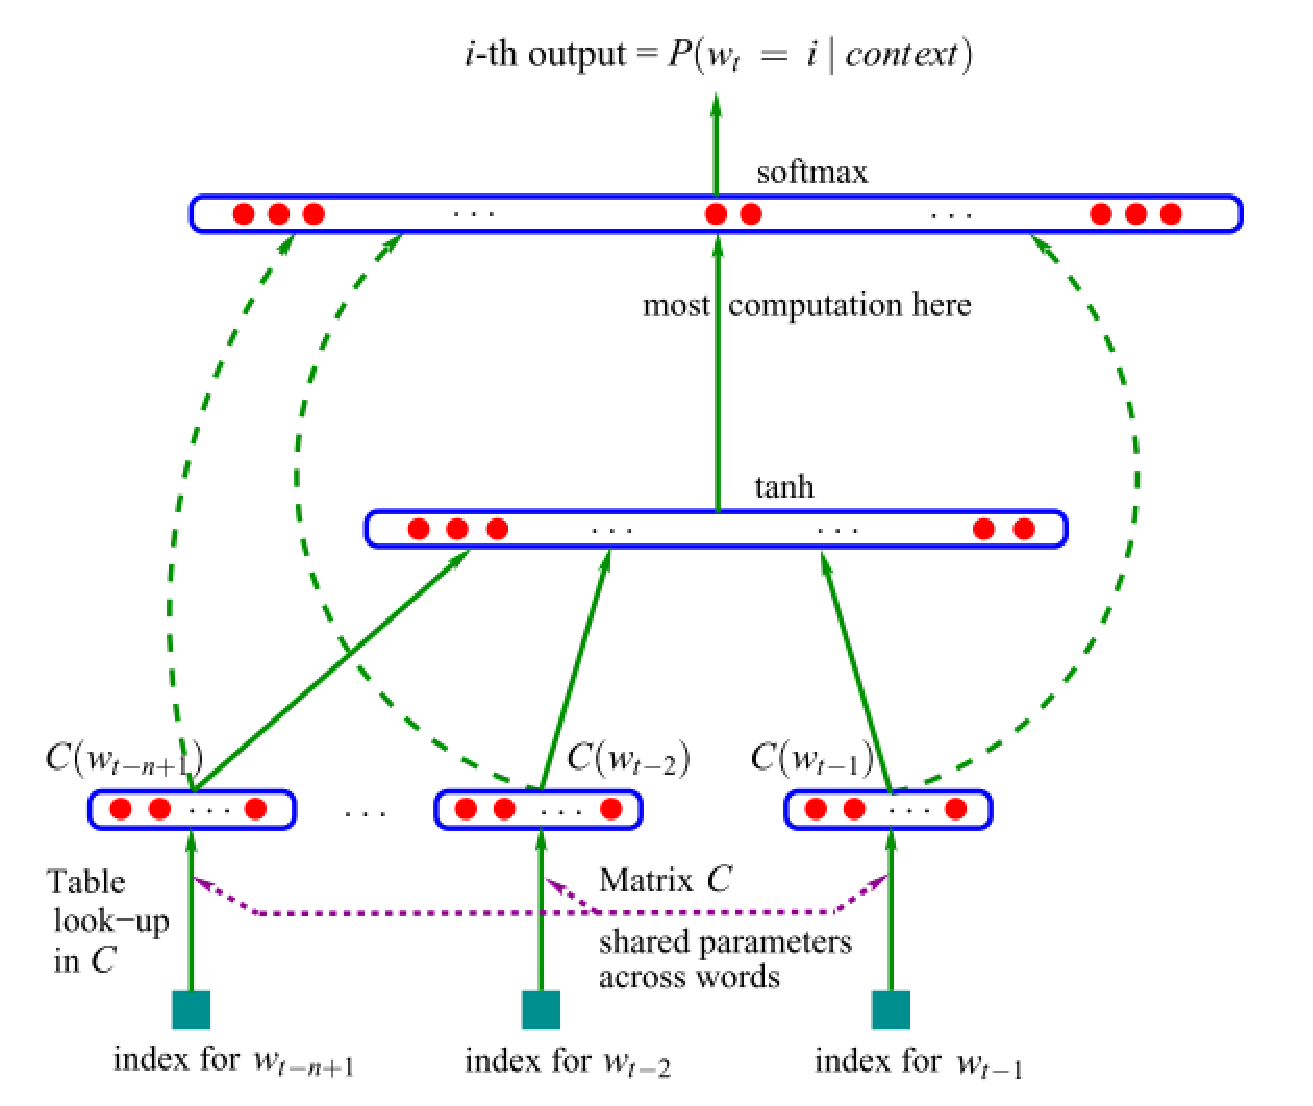
\includegraphics[width=.8\linewidth]{8_15_DL}\\
  \caption{An overview of the network architecture}\label{fig:DL}
\end{figure}

Figure \ref{fig:DL} shows the proposed neural architecture. The objective  function $f$ is a composition of $C$ and $g$, with $C$ being shared across all the words in the context. The function $g$ can be implemented by a feed-forward or recurrent neural network. This paper uses the ordinary hyperbolic tangent hidden layer with a softmax output layer.

The paper also explores parallelization on two types of platforms: shared-memory processor machines and Linux clusters with a fast network. In the case of a shared-memory processor, each processor works on a different subset of the data. Each processor computes the gradient for its examples, and performs stochastic gradient updates on the parameters of the model, which are simply stored in a shared-memory area. If the parallel computer is a network of CPUs, the paper chooses to parallelize across the parameters of the output units. The CPUs need to communicate the normalization factor of the output softmax, and the gradients on the hidden layer with the word feature layer. All the CPUs will duplicate the computations that precede the output units. After this step, each processor works on its local data as before.

In this experimental section, the paper measures the perplexity of the proposed model, and compares the results with several previous work. It is reported that the proposed method outperforms the most competitive alternative approach by up to 24\% in perplexity. 
\subsection{Stochastic language generation in dialogue using recurrent neural networks with convolutional sentence reranking \cite{Wen2015a}}

The task is to maps system acts into surface texts. The paper uses RNN LM to generate responses by sampling words from the predicted distribution conditioned on dialogue acts. After generating response candidates, CNN and RNN are used together to score and rerank the candidates. 
\subsection{Generating Text with Recurrent Neural Networks \cite{Martens2011}}

This paper proposes a new variant of \emph{Recurrent Neural Network (RNN)} called \emph{Multiplicative Recurrent Neural Network (MRNN)}, and demonstrates its power by applying it to character-level language modeling tasks. Specifically, the paper will use the MRNNs to predict the next character in a stream of text.

The standard RNN is formalized as follows: Given a sequence of input vectors $(x_1, ..., x_T)$, the RNN computes a sequence of hidden states $(h_1, ..., h_T)$ and a sequence of outputs $(o_1, ..., o_T)$ by iterating the following equations:
\begin{eqnarray}
h_t &=& tanh(W_{hx}x_t + W_{hh}h_{t-1} + b_h)\\
o_t &=& W_{oh}h_t + b_o
\end{eqnarray}

In the standard RNN the current input $x_t$ is first transformed via the weight matrix $W_{hx}$ and then contributes \emph{additively} to the hidden state, while the basic idea of MRNN is to allow the current input determine the entire hidden-to-hidden matrix ($W_{hh}$). Before going further, it is worthy to explain the motivation of this approach.

\begin{figure}[htbp]
  \centering
  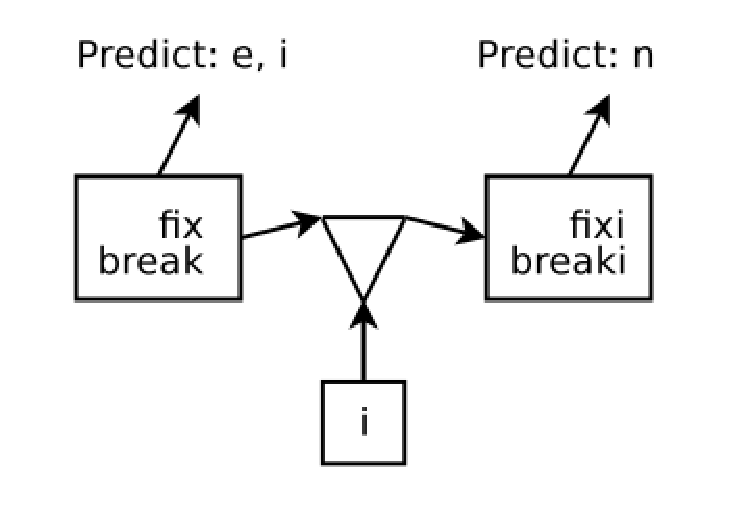
\includegraphics[width=.5\linewidth]{8_1_mrnn}\\
  \caption{A example that requires multiplicative connection}\label{fig:mrnn}
\end{figure}

For example in Figure \ref{fig:mrnn}, the character string ``ing'' is quite probable after ``fix'' and also quite probable after ``break''. If the hidden state vectors of the two words share a common concept of the stem of a verb, then there is a common representation to allow the character ``i'' to produce ``n''. Any evidence alone (verb stem or character ``i'') is not sufficient to make the prediction, and adding the weight additively is intuitively not a good strategy.

Based on the above analysis, in MRNN the update rule of hidden state vectors is changed to:
\begin{eqnarray}
h_t &=& tanh(W_{hx}x_t + W^{(x_t)}_{hh}h_{t-1} + b_h)
\end{eqnarray}
Here $W_{hh}$ is replaced with $W_{hh}^{(x_t)}$, allowing each character to specify a different hidden-to-hidden weight matrix.

The above scheme has a major drawback, which is that the storage required for $W_{hh}^{(x_t)}$ becomes prohibitive when the dimensionality of $x_t$ is even moderately large. The paper overcomes this problem by factoring $W_{hh}^{(x)}$ with three matrices $W_{fx}, W_{hf}$ and $W_{fh}$:
\begin{eqnarray}
W_{hh}^{(x_t)} = W_{hf} \cdot diag(W_{fx}x_t) \cdot W_{fh}
\end{eqnarray}
As a result, the updating rules can be represented as:
\begin{eqnarray}
f_t &=& diag(W_{fx}x_t) \cdot W_{fh}h_{t-1}\\
h_t &=& tanh(W_{hf}f_t + W_{hx}x_t)\\
o_t &=& W_{oh}h_t + b_o
\end{eqnarray}

In the experimental section, the paper makes comparison study with the \emph{sequence memorizer}  and \emph{PAQ}  methods. It is reported that MRNN achieves lower \emph{bits per character (bpc)} than the sequence memorizer but higher than PAQ (lower bpc implies better performance). The second part of experiment is to evaluate different methods with the \emph{debagging problem}, which is to convert a bag of words into a meaningful sentence. MRNN recovers the correct ordering 34\% of the time, which is higher than the memorizer (27\% of the time). Finally and most interestingly, the proposed neural network is used to generate sentence in character level, given a beginning of the sentence. For example, when initialized with the phrase ``The meaning of life is'', the MRNN generates the following sentence:

\begin{small}
The meaning of life is the tradition of the ancient human reproduction: it is less favorable to the good boy for when to remove her bigger. In the show's agreement unanimously resurfaced. The wild pasteured with consistent street forests were incorporated by the 15th century BE. In 1996 the primary rapford undergoes an effort that the reserve conditioning, written into Jewish cities, sleepers to incorporate the .St Eurasia that activates the population. Mar??a Nationale, Kelli, Zedlat-Dukastoe, Florendon, Ptuos thought is. To adapt in most parts of North America, the dynamic fairy Dan please believes, the free speech are much related to the...
\end{small}

\subsection{Recurrent Neural Network based Language Model \cite{Mikolov2010}}

This paper proposes a new \emph{recurrent neural network based language model (RNN LM)} with applications to speech recognition. Experimental results indicate that it reduces 50\% perplexity by using mixture of several RNN LMs, and speech recognition experiments show around 18\% reduction of word error rate on the Wall Street Journal task.

This paper uses an architecture that is usually called a \emph{simple recurrent neural network}, which is probably the simplest possible version of RNN, and very easy to implement and train. Let the input to the network at time $t$ be $x(t)$, output is denoted as $y(t)$, and $s(t)$ is the state of the network (hidden layer). Let $\oplus$ denote the concatenating operator. The simple recurrent neural network works by iterating the following equations:
\begin{align*}
x(t) &= w(t) \oplus s(t-1)\\
s_j(t) &= \sigma(\sum_i x_i(t) u_{ji})\\
y_k(t) &= softmax(\sum_j s_j(t) v_{kj})
\end{align*}

At each training step, error vector is computed according to cross entropy criterion and weighs are updated with the standard backpropagation algorithm.

The paper further suggests that the network should continue training even during testing phase, and refers to such model as \emph{dynamic}. While in training phase all data are presented to network several times in epochs, dynamic model gets updated just once as it processes testing data. It is shown that such simple technique is enough to obtain large perplexity reductions against static models. Dynamically updated models can thus automatically adapt to new domains.

In the experimental study, the paper evaluates the proposed method on several standard speech recognition tasks. On the WSJ corpus, the proposed model reduces WER by 18\% against 5-gram model with modified Kneser-Ney smoothing. Perplexity reductions are one of the largest ever reported (almost 50\%). In another experiment on the NIST RT05 corpus, it is shown that the proposed model trained on just 5.4M words can outperform backoff models that are trained on hundreds times more data.

\subsection{Energy-Based Models and Boltzmann Machines \cite{Bengio2009}}

In this survey we present the fifth chapter of the book \emph{Learning Deep Architectures for AI} by Bengio \cite{Bengio2009}. This chapter introduces the main mathematical concepts helpful to understand \emph{Restricted Boltzmann Machines (RBMs)}, which are particular energy-based models.

Energy-based models associate a scalar energy to each configuration of the variables of interest. For example, we would like plausible or desirable configurations to have low energy. The probability distribution of an energy-based model may be defined as follows:
\begin{equation}\label{equ:1}
P(x) = \frac{e^{-Energy(x)}}{Z}.
\end{equation}
Here $Z$ is a normalization term called the \emph{partition function} by analogy with physical systems.

In the \emph{products of experts} formulation, the energy function is a sum of terms, each one associated with an ``expert'' $f_i$:
\begin{equation}
Energy(x) = \sum_i f_i(x).
\end{equation}
Each expert can thus be seen as a detector of implausible configurations of $x$, or equivalently, as enforcing constraints on $x$.

In many cases we do not observe all the components simultaneously, or we want to introduce some non-observed variables to increase the expressive power of the model. So we consider an observed part $x$ and a hidden part $h$:
\begin{eqnarray}
P(x,h) = \frac{e^{-Energy(x,h)}}{Z},\\
P(x) = \sum_h P(x,h).
\end{eqnarray}
In order to map this formulation to the standard form, we introduce the notation of \emph{free energy}:
\begin{eqnarray}
P(x) = \frac{e^{-FreeEnergy(x)}}{Z},\\
FreeEnergy(x) = - \log \sum_h e^{-Energy(x,h)}.
\end{eqnarray}

The average log-likelihood gradient over the training set is
\begin{eqnarray}
E_{\hat{P}}[\frac{\partial \log P(x)}{\partial \theta}] = - E_{\hat{P}}[\frac{\partial FreeEnergy(x)}{\partial \theta}] + E_P[\frac{\partial FreeEnergy(x)}{\partial\theta}],
\end{eqnarray}
where expectations are over $x$, with $\hat{P}$ the training set empirical distribution and $E_P$ the expectation under the model's distribution.

If the energy can be written as a sum of terms associated with at most one hidden unit:
\begin{eqnarray}
Energy(x,h) = -\beta(x) + \sum_i \gamma_i(x, h_i),
\end{eqnarray}
then the free energy and numerator of the likelihood can be computed tractably:
\begin{eqnarray}
P(x) = \frac{e^\beta(x)}{Z} \prod_i \sum_{h_i} e^{-\gamma_i(x, h_i)}.
\end{eqnarray}

The \emph{Boltzmann machine} is a particular type of energy-based model with hidden variables. In a Boltzmann machine, the energy function is a general second-order polynomial:
\begin{eqnarray}
Energy(x,h) = -b'x - c'h - h'Wx - x'Ux - h'Vh.
\end{eqnarray}
The gradient of the log-likelihood can be written as:
\begin{eqnarray}
\frac{\partial \log P(x)}{\partial \theta} = - \sum_h P(h|x) \frac{\partial Energy(x,h)}{\partial \theta} + \sum_{\hat{x},h} P(\hat{x}, h) \frac{\partial Energy(\hat{x},h)}{\partial \theta}.
\end{eqnarray}
This gradient can be computed, if we have a procedure to sample from $P(h|x)$ and from $P(x,h)$. The basic idea is to use \emph{Gibbs sampling} in two phases: in the \emph{positive phase}, $x$ is clamped to the observed input vector, and we sample $h$ given $x$; in the \emph{negative phase} both $x$ and $h$ are sampled. Since two \emph{MCMCs (Monte Carlo Markov Chain)} (one for the positive phase and one for the negative phase) are needed for each example $x$, the computation can be very expensive.

\begin{figure}[h]
  \centering
  % Requires \usepackage{graphicx}
  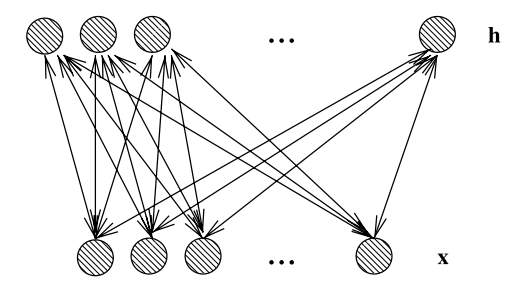
\includegraphics[width=.6\linewidth]{Bengio09-RBM.png}\\
  \caption{Undirected graphical model of a RBM}\label{fig:Bengio09}
\end{figure}

In the \emph{Restricted Boltzmann Machine (RBM)}, the $h_i$ are independent of each other when conditioning on $x$, and the $x_j$ are independent of each other when conditioning on $h$ (cf. Figure \ref{fig:Bengio09}). The energy function is bilinear:
\begin{eqnarray}
Energy(x,h) = -b'x - c'h - h'Wx.
\end{eqnarray}
The free energy of the input can be computed efficiently:
\begin{eqnarray}
FreeEnergy(x,h) = -b'x - \sum_i \log \sum_{h_i} e^{h_i(ci + W_i x)}.
\end{eqnarray}
Using the same factorization trick, we can obtain a tractable expression for $P(h|x)$ and $P(x|h)$.

Gibbs sampling in fully connected Boltzmann Machines is slow because there are as many sub-steps in the Gibbs chain as there are units in the network. The Factorization enjoyed by RBMs bring two benefits: 1) we do not need to sample in the positive phase because the free energy is computed analytically; 2) the set of variables $(x,h)$ can be sampled in two sub-steps in each step of the Gibbs chain: first we sample $h$ given $x$, and then a new $x$ given $h$.

\emph{Contrastive Divergence (CD)} is an approximation of the log-likelihood gradient that has been found to be a successful update rule for training RBMs. The basic idea of $k$-step CD is simple, and involves a second approximation, which introduces some bias in the gradient: run the MCMC chain $x_1, ..., x_{k+1}$ for only $k$ steps starting from the observed example $x_1 = x$. The surprising empirical result is that even $k=1$ often gives good results.


\subsection{Three New Graphical Models for Statistical Language Modelling \cite{Mnih2007}}

This paper shows how real-valued distributed representations for words can be learned at the same time as learning a large set of stochastic binary hidden features that are used to predict the distributed representation of the next word from previous distributed representations. One of the proposed models significantly outperforms the best $n$-gram models.

The first model is called the \emph{Factored Restricted Boltzmann Machine Language Model (FRBM)}. Each word is represented using a real-valued feature vector of length $N_f$. Let $R$ be an $N_w \times N_f$ matrix with row $i$ being the feature vector for the $i$-th word. The \emph{joint energy} of a sequence of words $w_1, ..., w_n$ is defined as:
$$E(w_n, h; w_{1:n-1}) = -(\sum_{i=1}^n v_i^T R W_i)h.$$
Here matrix $W_i$ specifies the interaction between the vector of hidden variables and the feature vector.

The joint conditional distribution of the next word and the hidden configuration $h$ is defined in terms of the energy function as:
$$P(w_n, h | w_{1:n-1}) = \frac{1}{Z_c} \exp(-E(w_n,h; w_{1:n-1})),$$
where $Z_c$ is a context-dependent normalization term. The conditional distribution of the next word can be obtained by marginalizing over the hidden variables.
\begin{figure}
  \centering
  % Requires \usepackage{graphicx}
  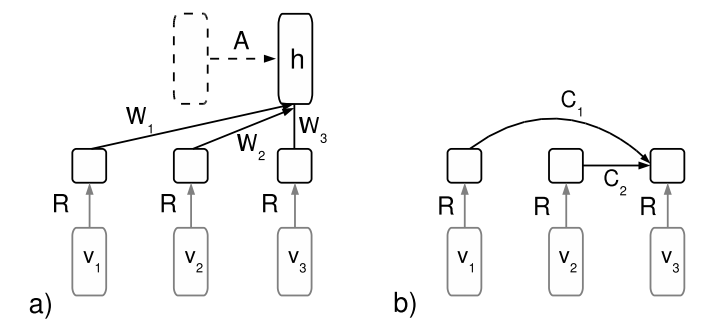
\includegraphics[width=.6\linewidth]{Minh07-RBM.png}\\
  \caption{a) The diagram for FRBM and TFRMB. The dashed part is included only for the TFRBM; b) The diagram for the log-bilinear model.}\label{fig:Minh07-RBM}
\end{figure}

The second model is called the \emph{Temporal Factored RBM (TFRBM)}. The basic idea is to make a simple extension to the factored RBM language model. Suppose we want to predict word $w_{t+n}$ from $w_1, ..., w_{t+n-1}$ for some large $t$. The method applies a separate instance of the model to words $w_\tau, ..., w_{\tau+n-1}$ for each $\tau$ in $\{1, ..., t\}$. In order to propagate context information forward, it further introduces directed connections from $h^\tau$ to $h^{\tau+1}$, and computes the hidden state of model $\tau+1$ using the inputs from the hidden state of model $\tau$ as well as its visible units. Figure \ref{fig:Minh07-RBM} (a) shows the diagram for the temporal FRBM.

The third model is called the \emph{log-bilinear language model}. The energy function of this model is specified as:
$$E(w_n; w_{1:n-1}) = -(\sum_{i=1}^{n-1} v_i^T R C_i)R^T v_n - b_r^T R^T v_n - b^T_v v_n.$$
In the FRBM energy function the interaction is between the word feature vectors and the hidden variables, whereas in this model the interaction is between the feature vectors for the context words and the feature vector for the predicted word. Intuitively, the model predicts a feature vector for the next word by computing a linear function of the context word feature vectors. Then it assigns probabilities to all words in the vocabulary based on the similarity. This model is similar to the energy-based model proposed in \cite{Bengio2003A}. However, the model proposed here uses a bilinear energy function, while the energy function in \cite{Bengio2003A} is a one-hidden-layer neural network. Figure \ref{fig:Minh07-RBM} (b) shows a diagram of the log-bilinear language model.

In the experimental study, the paper evaluates the proposed models using the \emph{Associated Press News (APNews)} dataset consisting of a text stream of about 16 million words. In the first experiment, it is shown that three of the four network models are competitive with $n$-gram models. The best results were obtained by averaging with the temporal network model, resulting in 21\% reduction in perplexity over the best $n$-gram model. In the second experiment, it is also shown that the log-bilinear models clearly outperform the $n$-gram models.


\section{Text-to-speech Synthesis} \label{Text-to-speech Synthesis}

The goal of the TTS component is to map a text to a waveform output. Speech synthesis systems typically perform this mapping in two steps, first converting the input text into a phonemic internal representation and then converting this internal representation into a waveform \cite{Jurafsky2006}.

We begin this section with a brief survey of the mature approach that are widely applied in commercial systems \cite{Jurafsky2006}. The most successful TTS systems that are widely used in commercial systems generally follow two approaches: the HMM-based method, and the unit selection method \cite{Black97}. When the TTS system is used in a limited domain (e.g. a weather report system), it is possible to make the voice more natural with some special techniques \cite{Black2000}. In the last paper, we introduce an end-to-end TTS system that works without explicit internal representation \cite{Wu2016Investigating}. This new line of research still awaits to be further explored, and is not among the mainstreams of commercial TTS systems.

\subsection{Speech Synthesis \cite{Jurafsky2006}}

This section is a summary of Chapter 8, Speech Synthesis of the book Speech and Language Processing \cite{Jurafsky2006}. In this summary we will see some main challenges and classic approaches of the \emph{text-to-speech (TTS)} task.

\begin{figure}[htbp]
  \centering
  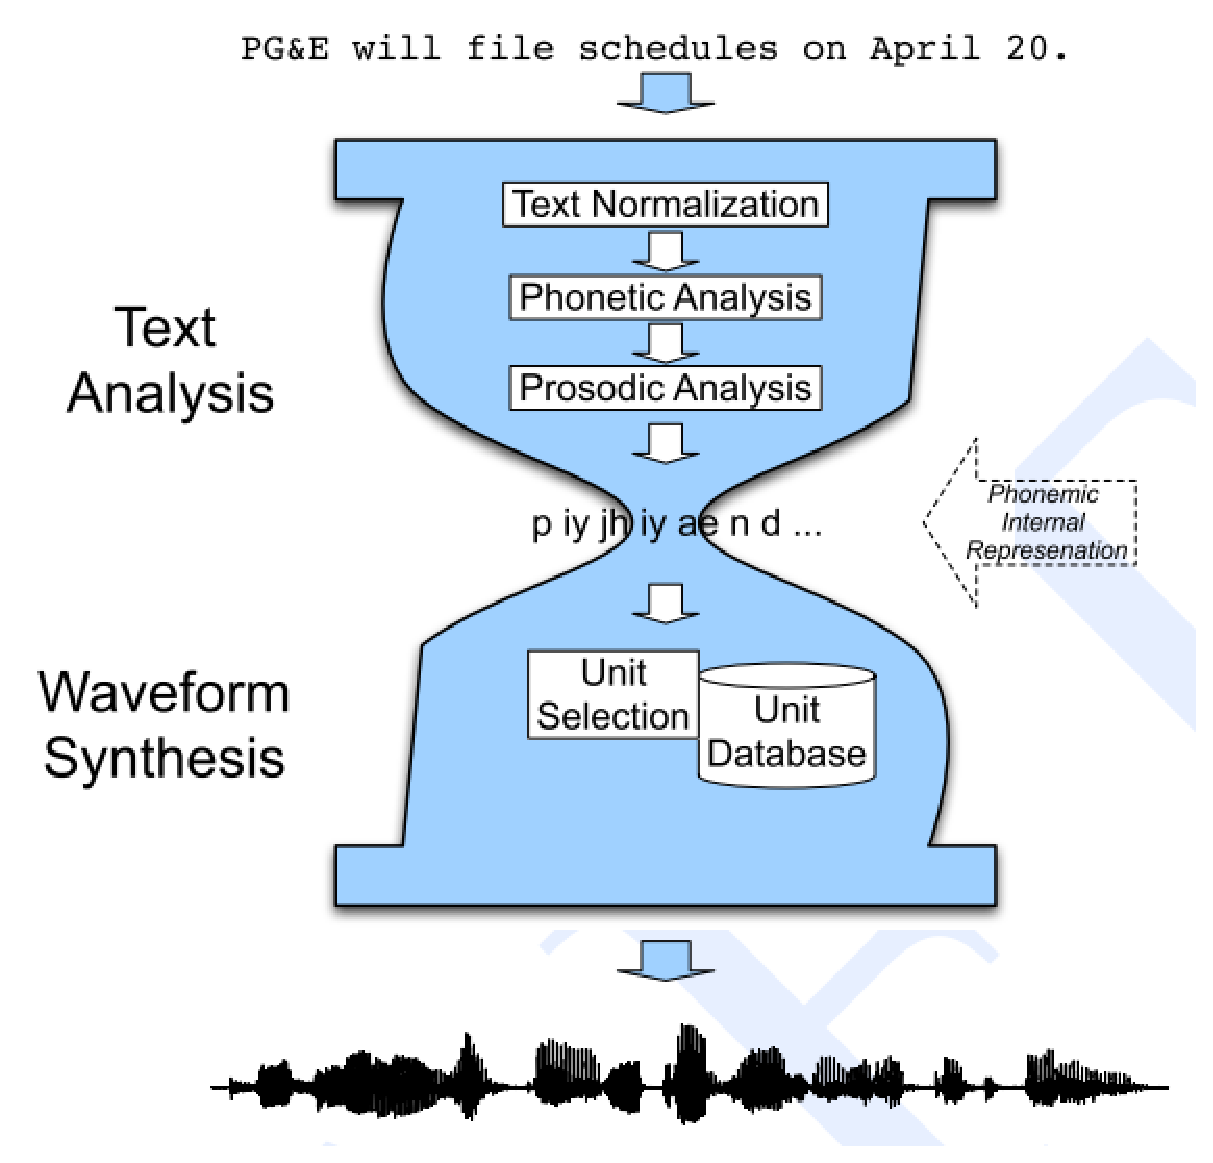
\includegraphics[width=.5\linewidth]{10_17_tts_arch}\\
  \caption{Architecture for the classic TTS system}\label{fig:TTS_arch}
\end{figure}

The goal of TTS is to map a text to a waveform output. The classic TTS architectures have two main steps, text analysis and waveform synthesis, as shown in Figure \ref{fig:TTS_arch}. While text analysis algorithms are relatively standard, there are three different paradigms for waveform synthesis: concatentative synthesis, formant synthesis and articulatory synthesis. Most modern commercial TTS systems are based on concatentative synthesis. Next we will explore each of the sub-tasks in further details.

The text analysis step has three main components: the text normalization component, the phonetic analysis component, and the prosodic analysis component. Each of them performs the following sub-tasks:
\begin{enumerate}
\item{Text Normalization:
    \begin{itemize}
    \item Sentence tokenization: This step segments a paragraph into a set of sentences, so that the TTS can synthesis speech for each sentence separately.
    \item Process non-standard words: There are several types of non-standard words, including numbers, abbreviations, acronyms and so on. For example, in `The European economy in 1750', the number 1750 is translated to `seventeen fifty'. But in `The password is 1750', the number should be translated to `one seven five zero'.
    \item Homograph disambiguation: Some words with the same spelling may have different pronunciations. For example, the word live in `live in China' should be pronounced differently from that in `a live animal'.
    \end{itemize}
}
\item{Phonetic Analysis: This stage takes the normalized word strings and produces a pronunciation for each word.
    \begin{itemize}
    \item Dictionary lookup: The first step is to directly lookup each word in the phonetic dictionary. For example, a sample entry in the CMU Pronouncing Dictionary is ``TABLE - T EY1 B AH0 L'' (0 denotes unstressed, 1 denotes stressed).
    \item Process names: There are many types of names, such as names of people, locations, organisations, etc. Some of the names may not appear in the dictionary. In the step the system need to decide how to pronounce them.
    \item Grapheme-to-phoneme: In this stage, the system uses letter-to-sound rules to process the remaining words.
    \end{itemize}
}
\item{Prosodic Analysis: The goal of the prosody analysis stage is to decide the rhythm, accent, stress, tune and other aspects of the speech.
    \begin{itemize}
    \item Prosodic structure: For example in a single phrase `I wanted to go to London', there seems to be some prosodic phrase boundaries that split up the words as follows: `I wanted | to go | to London'.
    \item Prosodic prominence: In any spoken utterance, some words sound more prominent than others. The notion of prominence is generally captured by a marker called pitch accent. The following example shows accented words in capital letters: `I'm a little SURPRISED to hear it.'
    \item Tune: A very obvious example of tune in English is the difference between statements and yes-no question. Consider the statement `you know what I mean' and the question `you know what I mean?'.
    \item Compute duration and F0 from prosodic labels: F0 refers to the lowest frequency of a complex wave. Some algorithms such as the unit selection synthesis approach do not need this step.
    \end{itemize}
}
\end{enumerate}

\begin{figure}[htbp]
  \centering
  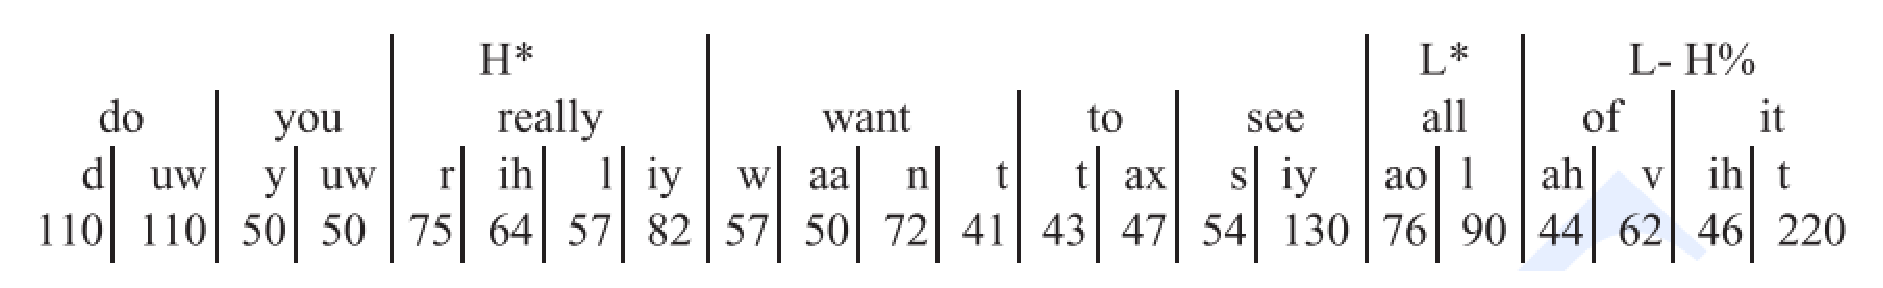
\includegraphics[width=.7\linewidth]{10_17_tts1}\\
  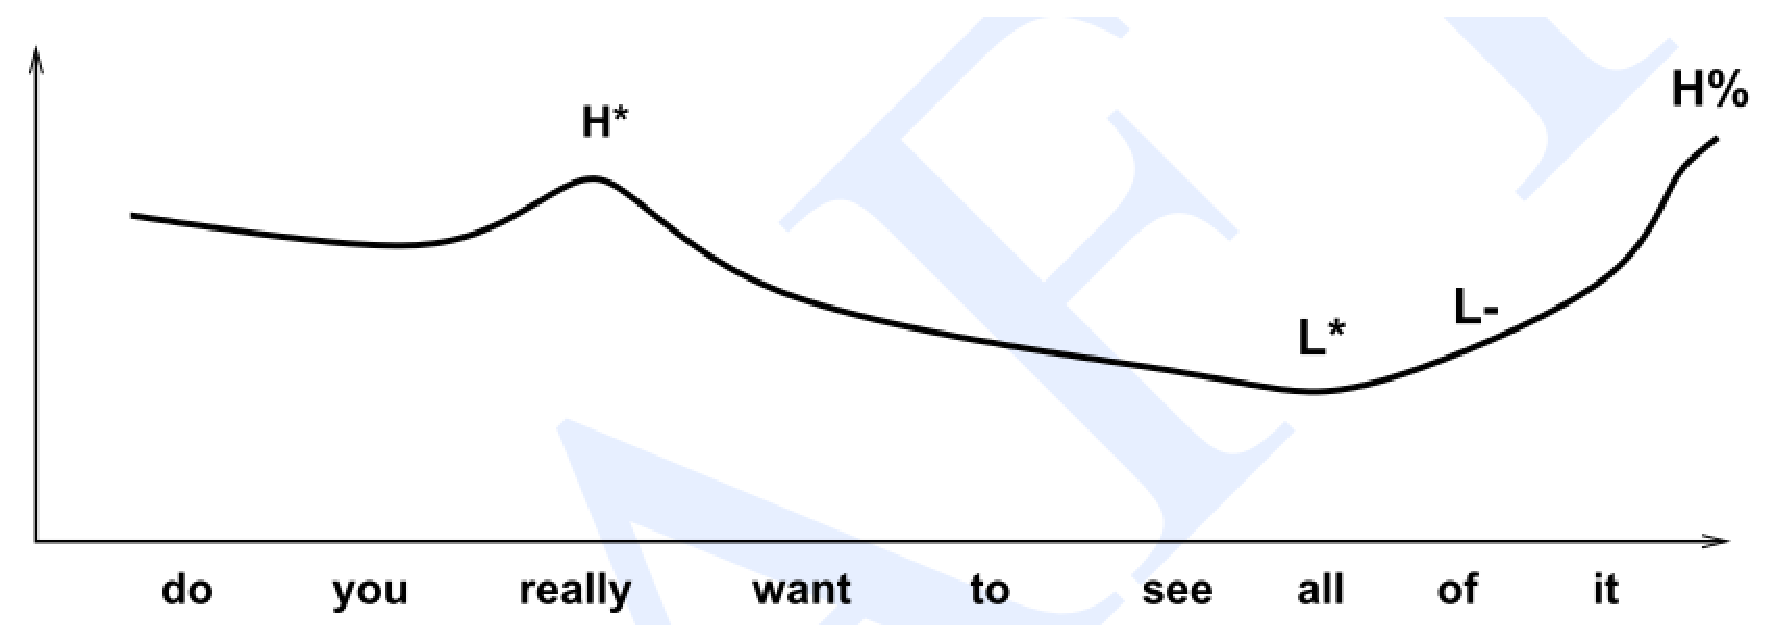
\includegraphics[width=.5\linewidth]{10_17_tts2}\\
  \caption{Internal representation of the FESTIVAL diphone system}\label{fig:TTS_inter}
\end{figure}

The final output of text analysis is called the internal representation of the input text sentence. Figure \ref{fig:TTS_inter} shows some TTS output from the FESTIVAL diphone system for the sentence `Do you really want to see all of it?'.

The next step is to turn the internal representation into a waveform. As aforementioned most of the modern commercial TTS systems are based on concatentative synthesis. The basic idea of concatentative approaches is to store the speech of human speakers in a database, and then retrieve and concatenate them according to the internal output. Two concatentative methods are discussed in this chapter: diphone synthesis and unit selection synthesis.

A diphone is a phone-like unit going from roughly the middle of one phone to the middle of the following phone. It takes a sequence of diphones from the database that corresponds to the desired phone sequence, and then concatenates them with some slight signal processing. Finally the algorithm performs some prosodic adjustments to the concatenated utterance.

Modern commercial TTS systems are based on a generalization of diphone synthesis, called unit selection synthesis. It differs from the classic diphone approach is two ways: 1) The unit selection database is much bigger (many hours long), containing many copies of each diphone; 2) Unit selection synthesis use no signal processing to the concatenated units, such as prosodic adjustments.

Finally, the section discusses some evaluation methods of the TTS systems. The development of a good automatic metric for speech synthesis remains an open question. Currently the speech synthesis systems are still evaluated by human listeners.

Remark: I think the TTS can be treated as an isolated component in our chatbot system. While it is intuitively beneficial to combine ASR and the dialogue manager (such as by jointly training), it seems difficult to improve TTS in a similar manner. I think we can use existing TTS system as a black box, without too much caring about how it works. 
\subsection{Unit Selection in Speech Synthesis \cite{Black97}}

This paper describes a new method for synthesizing speech by concatenating sub-word units from a database of labelled speech. The method is implemented within a full text-to-speech system, called the \emph{Festival}, offering efficient natural sounding speech synthesis.

In the selection based synthesis, there is a large database of speech with a variable number of units from a particular class. The goal of these algorithms is to select the best sequence of units from all the possibilities in the database, and concatenate them to produce the final speech.

The basic idea of the unit selection technique proposed in the paper is summarized as follows: 1) A large units inventory is created by automatically clustering units of the same phone class based on their phonetic and prosodic context; 2) The appropriate cluster is then selected for a target unit; 3) Finally an optimal path is found through the candidate units based on their distance from the cluster center and an acoustically based join cost.

The first step is to cluster the units. The paper defines an acoustic measure to measure the distance between two units of the same phone type, by using an acoustic vector which comprises Mel frequency cepstrum coefficients, $F_0$, power, etc. The acoustic distance between two units is simply the average distance for the vectors (including some frames in the previous units). The distance measure is used by the CART algorithm, which builds a decision tree whose questions best minimise the impurity of the sub-clusters.

To join consecutive candidate units from clusters selected by the decision trees, it uses an optimal coupling technique to measure the concatenation costs between two units. This technique offers two results: the cost of a join, and a position for the join. Optimal coupling allows it to select more stable positions towards the center of the phone.

At synthesis time the input is a stream of target segments to be synthesized. For each target it uses the CART for that unit type, and ask the questions to find the  appropriate cluster which provides a set of candidate units. Let $Tdist(U)$ be the distance of a unit $U$ to its cluster center, and the function $Jdist(U_i, U_{i-1})$ be the join cost. The proposed method uses a Viterbi search to find the optimal path through the candidate units that minimizes the following expression:
$$\sum_{i=1}^N Tdist(U_i) + W * Jdist(U_i, U_{i-1}).$$

The paper further discusses the pruning technique, which can reduce the size of the distributed database. Pruning has two effects: 1) remove spurious atypical units which may have been caused by mislabelling or poor articulation in the original recording; 2) remove those units which are so common that there is no significant distinction.

In the experimental study, the paper tries the proposed method with two databases: 1) TIMIT, a male British English speaker (about 14,000 units); 2) Boston University FM Radio corpus, a female American news reader (about 37,000 units). In the test it generated 20 sentences for each evaluated model. The sentences from each model were played against those from another set, and the subjects decide which ones are better. In this way, the author conducted comparison study by varying cluster size, $F_0$ weight in the acoustic cost, and the amount to prune final clusters. The empirically optimal parameters were respectively reported.

\subsection{Limited Domain Synthesis \cite{Black2000}}

This paper presents a reliable and efficient method for building limited domain speech synthesis voices. By constructing databases close to the target domain of the speech application, it uses \emph{unit selection} synthesis techniques to reliably give high quality synthesis within domain.

The task of building a voice consists of the following processes:
\begin{itemize}
\item{Design the corpus\\
The first step is to design a prompt list that adequately covers the domain. In general, prompts should have at least one occurrence of each word in the vocabulary in each prosodic context.
}
\item{Synthesize each utterance\\
The prompts are synthesized for a number of reasons: 1) ensure that all the tokens are expanded properly (e.g. flight numbers and dates); 2) estimate the time required for recording; 3) use the synthesized prompt in labeling the human spoken utterance.
}
\item{Record the voice talent\\
Recording with studio quality equipment gives better results, but the paper is also interested in making the process more accessible. It uses a laptop in a quiet room. The recording quality shows to be acceptable once audio devices are set up appropriately.
}
\item{Label the recordings\\
After recording, it labels the text using a simple but effective technique based on \cite{Malfrere1997}: it uses DTW to align between the mel-scale cepstral coefficients of the synthesized and recorded waveforms.
}
\item{Extract pitchmarks
}
\item{Extract pitch-synchronous parameters
}
\item{Build a cluster unit selection synthesizer\\
The unit selection technique used in this paper is an updated version of that more fully described in \cite{Black97}. The general algorithm takes all units of the same type and calculates an acoustic distance between each. Selected features including phonetic and prosodic context are used to build a decision tree that minimizes acoustic distance in each partition. At synthesis time, it selects the appropriate cluster using the decision tree, and then finds the best path through the candidates.
}
\item{Test and tune, repeating as necessary}
\end{itemize}

The proposed technique is tested on three domains: a talking clock, a weather report system, and the CMU Communicator system.

The original demonstration of this technique was a simple talking clock. The prompts consist of 24 simple utterances of the form: ``The time is now, a little after quarter past two in the afternoon.'' Not counting recording time, this takes around 3 minutes to build. Such clocks have also been built in languages other than English, such as Chinese.

The most difficult example is the CMU Communicator system. At first it appears that the domain is not closed, as it includes greeting to registered users by name, and allows reference to any airport in the world. For the words like cities and airports, which are essentially open classes, it used the frequency information in the logs to select which set to include in the recordings. For the more frequently mentioned cities it includes more than one occurrence in the prompts. The final voice was built in under one-man week. After the version was running, it made some changes to the language generation system, and constructed further 50 utterances and added them into the system in another morning's work.

\subsection{Investigating gated recurrent networks for speech synthesis \cite{Wu2016Investigating}}

Recently, \emph{recurrent neural networks (RNNs)} have re-emerged as a potential acoustic model for \emph{statistical parametric speech synthesis (SPSS)}. This paper attempts to answer two questions: 1) why do LSTMs work well as a sequence model for SPSS; 2) which component of the LSTM unit is most important. It presents a visual analysis along the experiments, resulting in a simplified architecture.

The goal of the paper is to reach a better understanding of the ``black-box'' LSTM architecture. First, it gives an analysis of the forget gate and memory cell in the LSTM architecture. Specifically, it visualises the activation of the forget gate to understand when the forget gate resets the memory cell state, and how the forget gate relates to speech structure. Second, it analyses the importance of each LSTM component (e.g., input gate, output gate, forget gate), and proposes a simplified architecture.

To assess the importance of each component, the paper starts with four variants of the LSTM architecture: 1) No Peep-holes (NPH): Set the peep-hole connections $p^i, p^o, p^f$ to zeros. 2) No input gate (NIP): Set the input gate to 1 ($i_t = 1$). 3) No forget gate (NFG): Set the forget gate to 1 ($f_t = 1$). 4) No output gate (NOG):  Set the output gate to 1 ($o_t = 1$).

\begin{figure}[htbp]
  \centering
  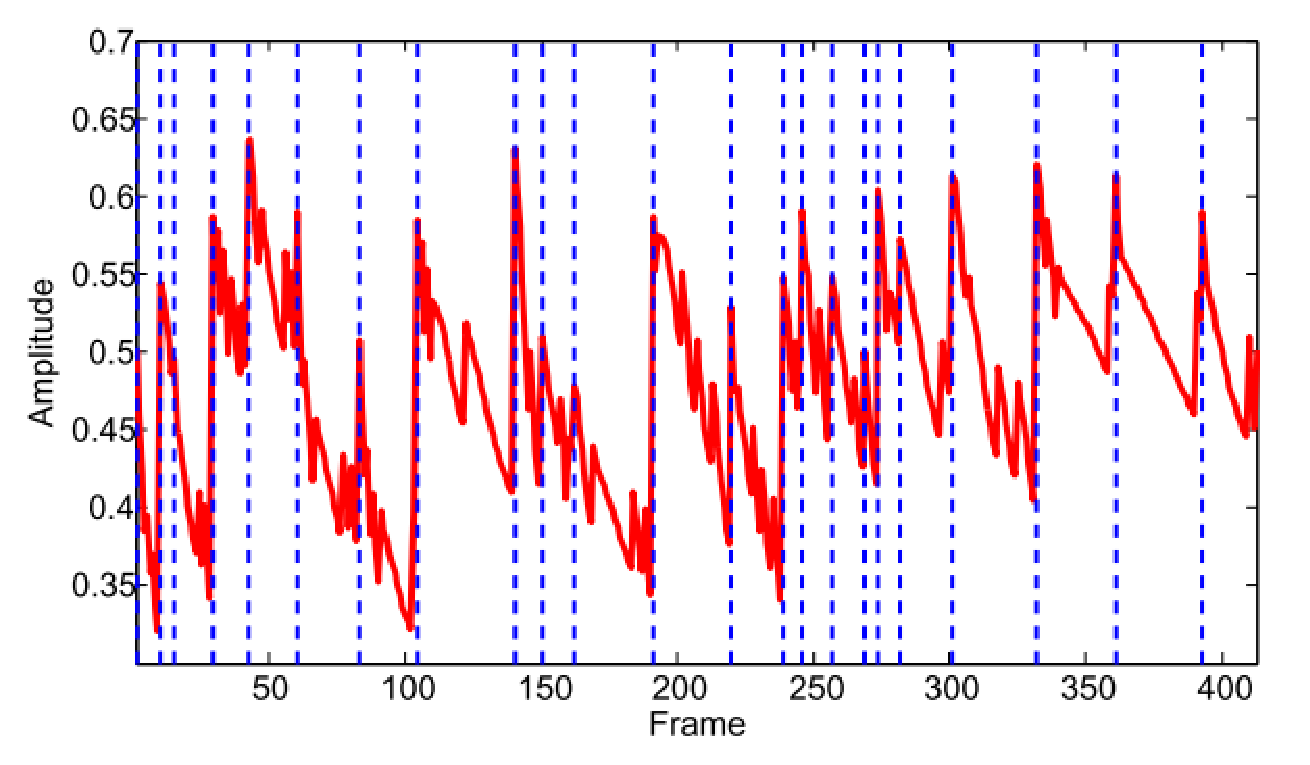
\includegraphics[width=.5\linewidth]{10_3_acu1}\\
  \caption{Averaged activations of all forget gates}\label{fig:acu1}
\end{figure}

\begin{figure}[htbp]
  \centering
  % Requires \usepackage{graphicx}
  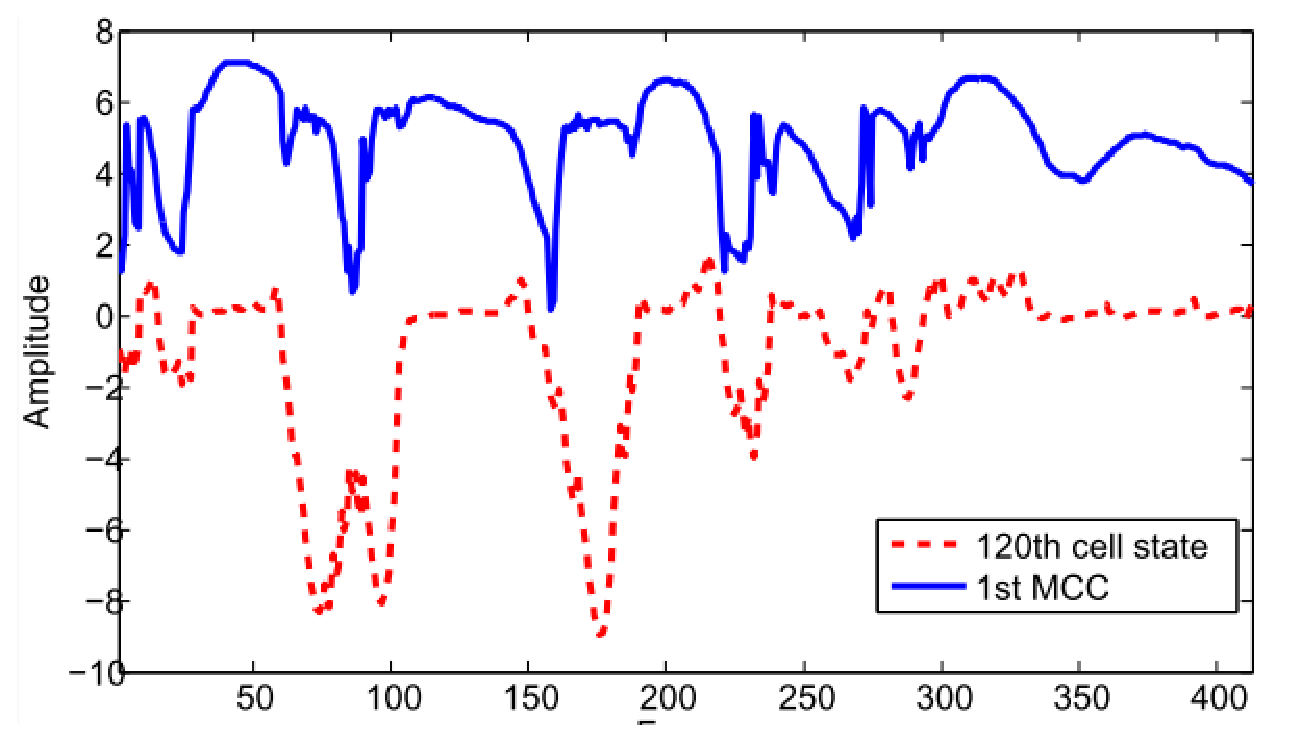
\includegraphics[width=.5\linewidth]{10_3_acu2}\\
  \caption{Comparison between the Mel-Cepstral Coefficient (MCC) trajectory and a cell state}\label{fig:acu2}
\end{figure}

The first step of the analysis is to visualise the forget gate and cell state, which are thought to be the two most important components in modelling long-term temporal structure. The averaged activations over the 256 units of the forget gate are presented in Figured \ref{fig:acu1}. It can be observed that the peaks of the forget gate activation trajectory have a strong correspondence with the phoneme boundaries. The memory cell should store the trend of the trajectory to be predicted, and a comparison between the relation is presented in Figure \ref{fig:acu2}.

The objective experiment compares the standard LSTM with different variations. The results show that the NFG system increases distortion considerably, which implies that the forget gate is the most important. Based on this observation, the paper proposes a simplified LSTM structure, which removes output gates and peep-hole connections, and replaces the input gate by the forget gate. The other experimental results also shows that the simplified LSTM is as good as any other systems.

Remark: This paper provides a detailed analysis of the performance of different components of the LSTM unit. In many occasions, we tend to use network architectures like LSTM as black boxs - we believe that they would work well because they are successful in other tasks. This paper reminds us that it is still necessary to look into why a network works on a specific problem. This may bring us deeper insight, and probably result in a better architecture. 

\section{Non-goal-driven Systems} \label{Non-goal-driven Systems}

Non-goal-driven systems usually accomplish NLU, DM, and NLG jointly. Historically, they start as rule-based systems, such as ELIZA \cite{Weizenbaum1966Eliza} and ALICE \footnote{http://www.alicebot.org/}. As the amount of conversational corpus becomes large, data-driven systems have been researched since 2011 \cite{Ritter2011Data}. The methods used in data-driven systems fall into two categories: (1) Retrieval-based methods \cite{Ji2014An, Yan2016DocChat}; (2) Generation-based methods \cite{Ritter2011Data, Shang2015Neural, Sordoni2015a, Serban2016}. Non-goal-driven systems may be useful for goal-oriented systems when they are trained on corpus related to the tasks of goal-oriented systems: (1) They can be used as user simulator to construct large task-specific corpus; (2) They may directly act as goal-oriented systems \cite{Vinyals2015A}.

\subsection{A neural conversational model \cite{Vinyals2015A}.}

The task is to build end-to-end trainable chatbots that can have multiple rounds of domain-specific or open-domain conversations. The paper applies sequence-to-sequence learning, which uses an encoder to map the input sequence to a fixed-length vector, i.e. the hidden state, and uses a decoder LSTM to decode the output sequence from the vector \cite{Sutskever2014Sequence}.

The encoder that is a multilayer LSTM takes a sequence of words ($x_{1},...,x_{T}$):
\begin{equation}
h_{t} \ = \ f( h_{t-1}, x_{t} ) \\
\end{equation}

Given the last hidden state of encoder, $h_{T}$, the decoder that is another multilayer LSTM computes the probability of generating next word:
\begin{equation}
\begin{aligned}
s_{t} \ =& \ f( s_{t-1}, y_{t-1}, h_{T} ) \\
y_{t} \ =& \ g( s_{t} )
\end{aligned}
\end{equation}
where $g$ is a softmax function. The encoder stops after generating a special end-of-sentence symbol EOS.

When trained on a domain-specific IT trouble shooting dataset, the chatbot can solve users' IT problems via multi-round conversations. When trained on an open-domain movie transcript dataset, the chatbot can remember facts and common sense knowledge, perform simple forms of reasoning, etc. 
\subsection{Neural responding machine for short-text conversation \cite{Shang2015Neural}.}

The task is to build end-to-end trainable chatbots that can have one round conversations. The paper applies encoder-decoder framework, which uses GRU \cite{Chung2014Empirical, Cho2014Learning} encoders to encode the input post to a hidden state, and uses a GRU decoder to decode the output reply.

The encoders consist of a global encoder \cite{Chung2014Empirical, Cho2014Learning} and a local encoder \cite{Bahdanau2014Neural, Graves2013Generating}. The global encoder maps the input post to the last hidden state:
\begin{equation}
h_{t} \ = \ f( h_{t-1}, x_{t} ) \\
\end{equation}
where ($x_{1},...,x_{T}$) is a input sequence of words. The decoder uses $h_{T}$ as the context vector $c_{t}$

The local encoder maps the input post to weighted sum of hidden states when encoding the input post:
\begin{equation}
\begin{aligned}
h_{t} \ =& \ f( h_{t-1}, x_{t} ) \\
\alpha_{tj} \ =& \ q(s_{t-1}, h_{j}) \\
c_{t} \ =& \ \sum_{j=1}^{T} \alpha_{tj}h_{j} \\
\end{aligned}
\end{equation}

The decoder works as follows:
\begin{equation}
\begin{aligned}
s_{t} \ =& \ f( s_{t-1}, y_{t-1}, c_{t} ) \\
y_{t} \ =& \ g( s_{t} ) \\
\end{aligned}
\end{equation}
\subsection{Building end-to-end dialogue systems using generative hierarchical neural network models \cite{Serban2016}}

The task is to build end-to-end trainable chatbots that can have open-domain conversations. The paper applies HRED \cite{Sordoni2015a}, which uses encoder GRU \cite{Chung2014Empirical, Cho2014Learning} to encode the input utterance to an utterance vector, uses context GRU to map the utterance vector to a context vector, and uses decoder GRU to decode the context vector to generate the output response. The chatbots are improved by bootstrapping word embeddings from large news datasets with word2vec \cite{Mikolov2014Empirical}, or by pretraining model parameters on large QA datasets. The chatbots can also benefit from using bidirectional RNN \cite{Sundermeyer2014Translation}.



\bibliographystyle{ieeetr}
\bibliography{d:/research/chatbot}

\end{document}
